%%\paragraph{}
Due to the large contribution from the completely data-driven QCD background, it is important to model this background as good as possible in all regions of the analysis. Using the $1/2b$ region to model the $2bs$, $3b$, and $4b$ regions can introduce discrepancies in the modeling of the estimated QCD background versus the real n$b$ data. These discrepancies arise possibly from the non-trivial effect that $b$-tagging has on jet kinematics. The natural choice of reweighting variable is the $p_{T}$ of the track jets in the event, since these are the objects that we apply the $b$-tagging to. Also, large-$R$ jet $p_{T}$ is also reweighted to account for the effect from light and charm quark composition difference at different energy scales. The three chosen variables are the leading large-$R$ jet $p_{T}$, leading large-$R$ jet leading trackjet $p_{T}$ and subleading large-$R$ jet leading trackjet $p_{T}$.

%%\paragraph{}
In order to account for the $b$-tagging effect, a reweighting on the $1/2b$ data is adopted. The basic idea is to reweight the non $b$-tagged Higgs candidate to have kinematic distributions just like a $b$-tagged Higgs candidate. The idea is demonstrated in Figure~\ref{fig:rw-2bs-comp}. It shows that $2bs$ has very similar kinematic distributions on the trackjet \pt as the $1b$ sample, when the variable is the $b$ tagged trackjet. 

%%\paragraph{}
For $2bs$, the $1b$ non-tagged Higgs candidate is reweighted to be like a $1b$ tagged Higgs candiate; for $3b$, the $2b$ non-tagged Higgs candidate is reweighted to be like a $1b$ tagged Higgs candidate; for $4b$, the $2b$ non-tagged Higgs candidate is reweighted to be like a $2b$ tagged Higgs candidate. For each category, the events are split into two orthogonal subgroups, depending on whether leading/subleading Higgs candidate is $b$-tagged, the event is then reweighted such that the untagged Higgs candidate's distribution behaves like the corresponding $b$-tagged Higgs candidate's.

%%%%%%%%%%%%%%%%%%%%%%%%%%%
\begin{figure*}[htbp!]
\begin{center}
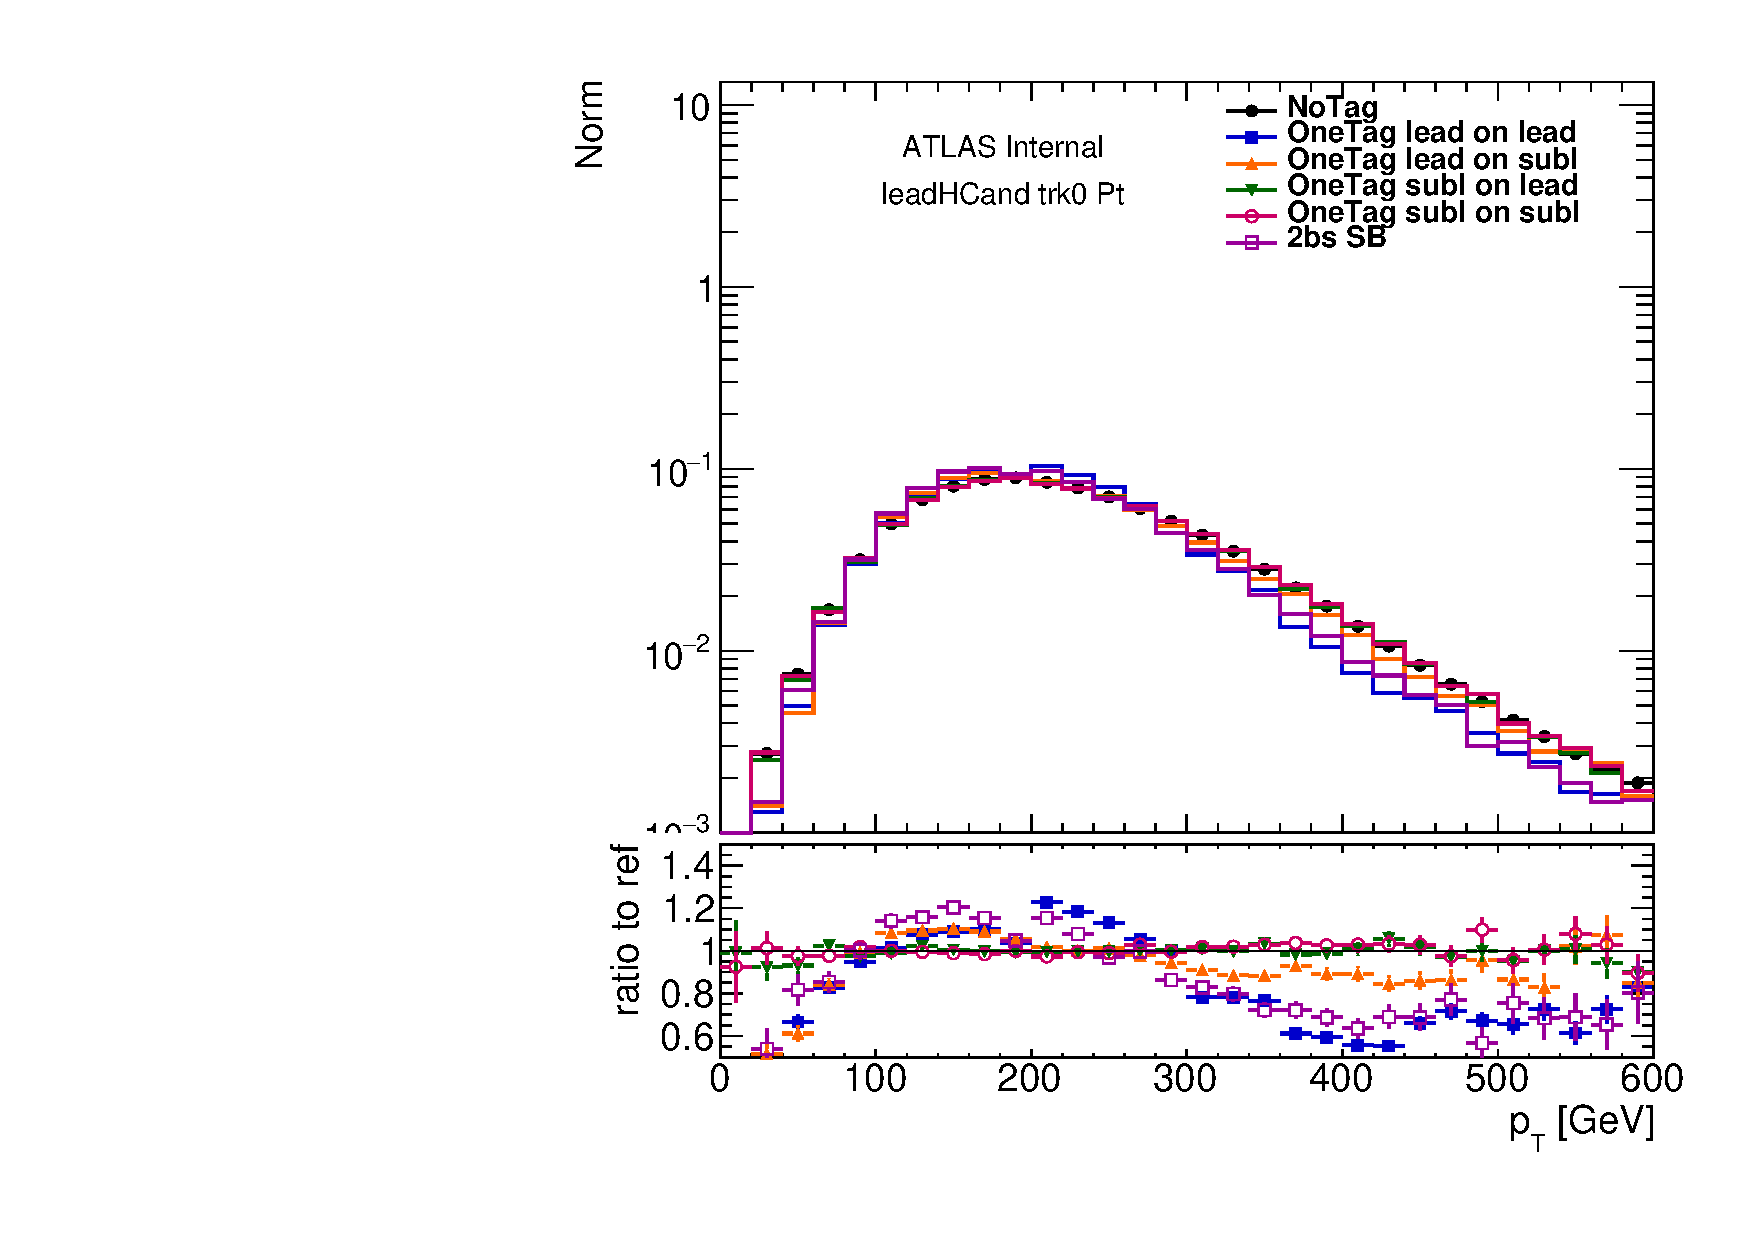
\includegraphics[width=0.4\textwidth,angle=-90]{figures/boosted/Prereweight/2bs_directcompare_leadHCand_trk0_Pt_1.pdf}
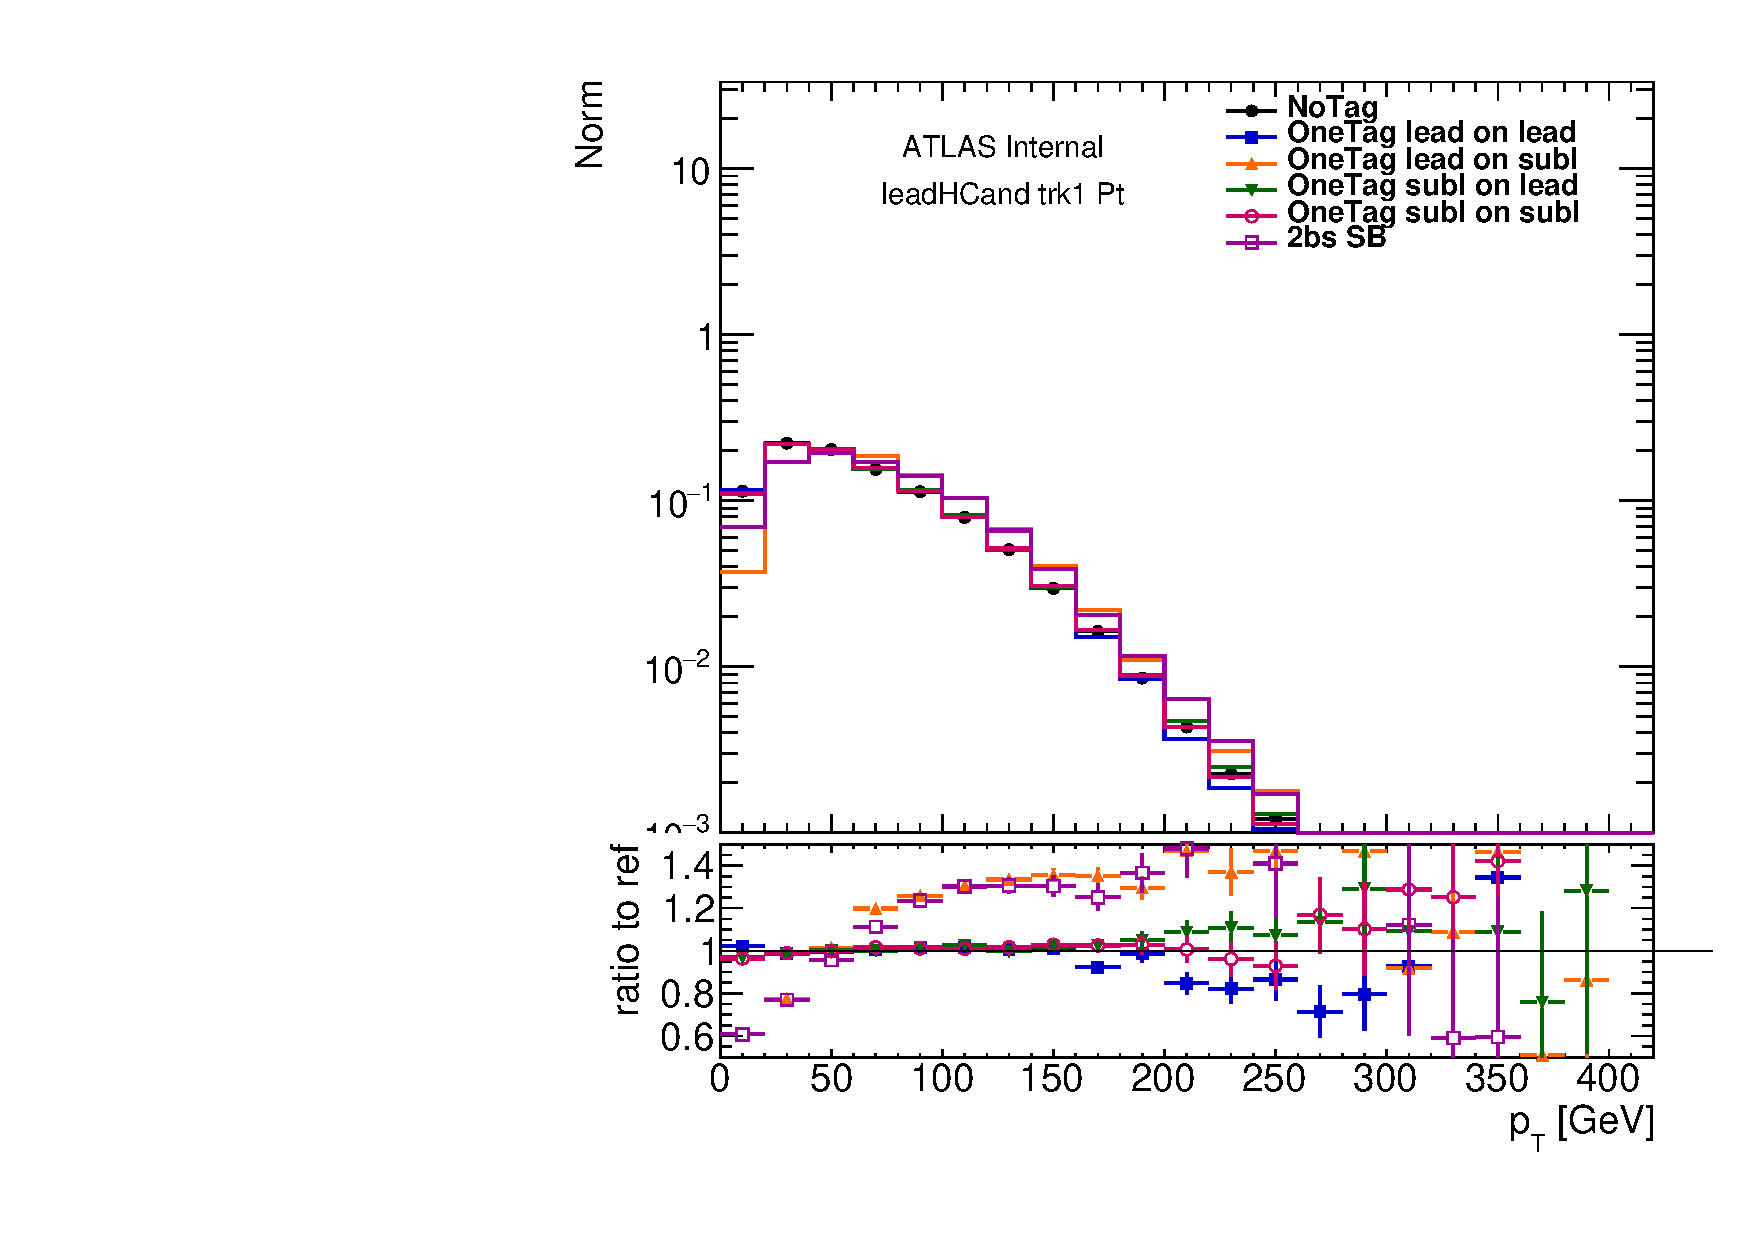
\includegraphics[width=0.4\textwidth,angle=-90]{figures/boosted/Prereweight/2bs_directcompare_leadHCand_trk1_Pt_1.pdf}\\
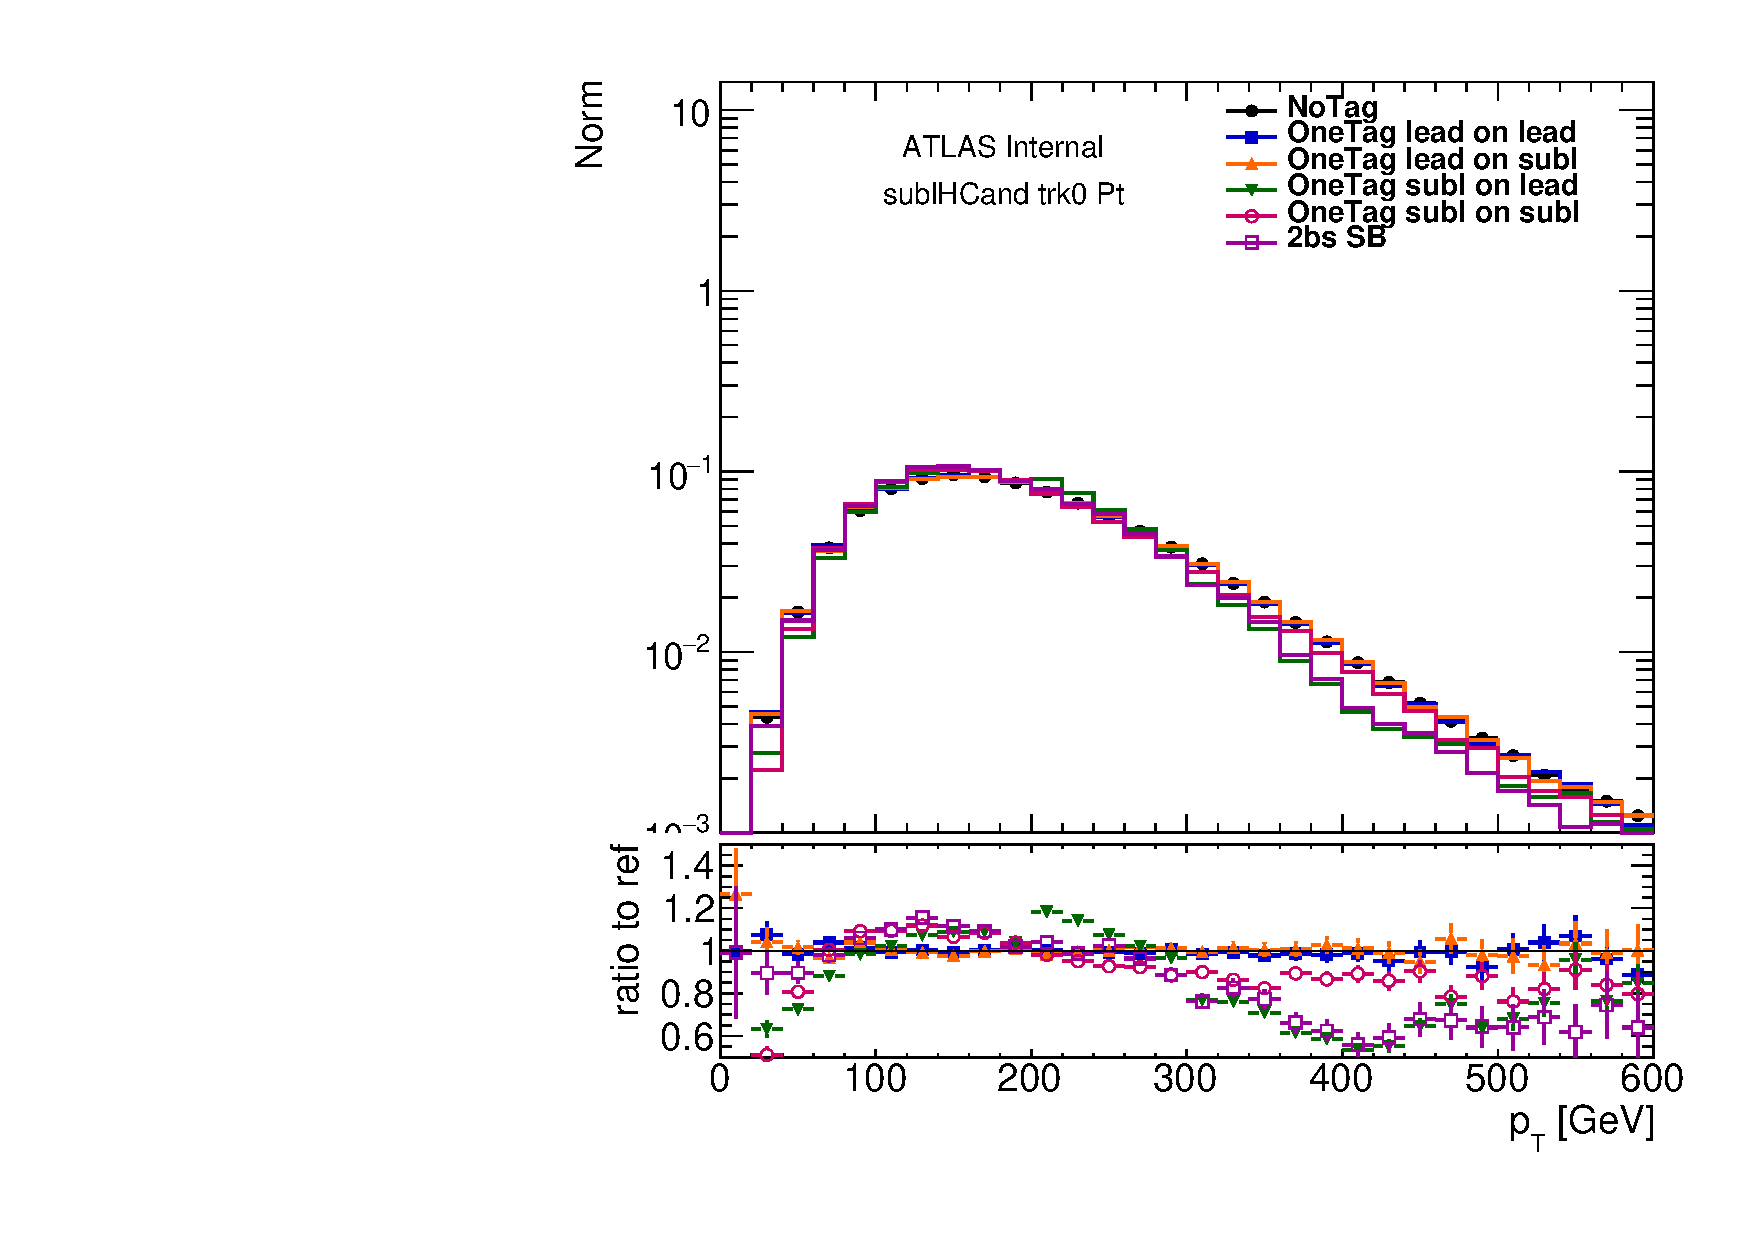
\includegraphics[width=0.4\textwidth,angle=-90]{figures/boosted/Prereweight/2bs_directcompare_sublHCand_trk0_Pt_1.pdf}
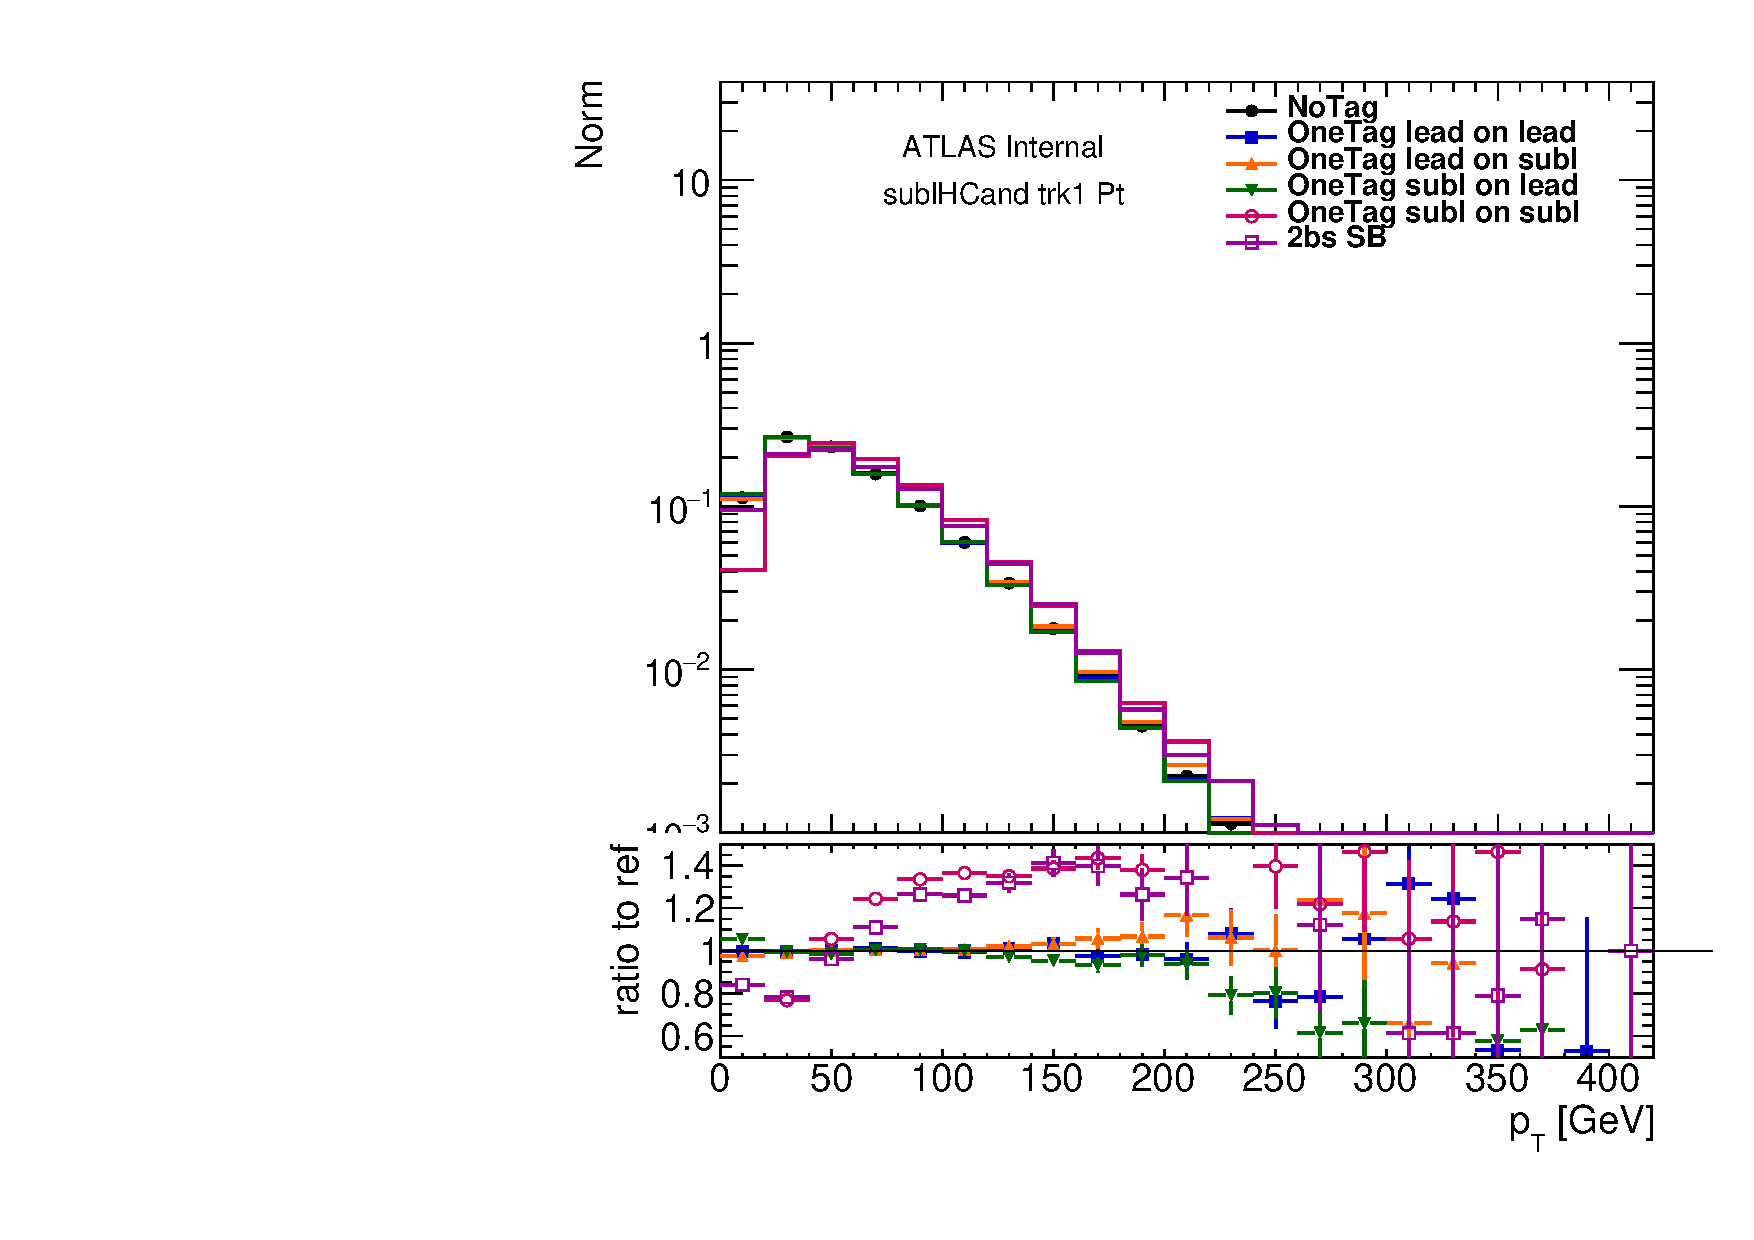
\includegraphics[width=0.4\textwidth,angle=-90]{figures/boosted/Prereweight/2bs_directcompare_sublHCand_trk1_Pt_1.pdf}\\
\caption{Comparison of different trackjet \pt distributions. Top row is for leading \pt Higgs candidate, and bottom row is for subleading \pt Higgs candidate. Left column is for the leading \pt trackjet of the Higgs candidate, and right column is for the subleading \pt trackjet of the Higgs candidate. Shown in the plot are just data distributions, inclusive of SB, CR, and SR regions for $0b$ and $1b$, while for $2bs$ only the SB region is shown. $1b$ sample is further split into four subcategories, depending on which trackjet gets $b$ tagged. OneTag lead on lead means the $b$ tagged trackjet is the leading trackjet of the leading Higgs candidate, OneTag lead on subl means the $b$ tagged trackjet is the subleading trackjet of the leading Higgs candidate, OneTag subl on lead means the $b$ tagged trackjet is the leading trackjet of the subleading Higgs candidate, and OneTag subl on subl means the $b$ tagged trackjet is the subleading trackjet of the subleading Higgs candidate. At the bottom ratio plot, all the ratio are taken with respect to the $0b$ tagged distribution.}
\label{fig:rw-2bs-comp}
\end{center}
\end{figure*}

%%\paragraph{}
To avoid potential biases in the final distributions used for the analysis, a reweighting technique is applied to the $1/2b$ data only. Since each signal region is modeled by a different $1/2b$ tag category: $2bs$ by $1b$ tag events with at least 1 track jets on both large-$R$ jets, $3b$ by $2b$ tag events with at least one track jets on one large-$R$ jet and at least two track jets on the other large-$R$ jet, and $4b$ by $2b$ tag events with at least two track jets on both large-$R$ jets, the reweighting procedure is the same but orthogonal for the three different channels. Note the $2b$ sample is already split into seperate parts, as described in paragraph \ref{par:boosted-qcd-2bseperate}.

\clearpage{}
%%\paragraph{}
The detailed procedure is listed as follows:
\begin{itemize}
\item Substracting $1/2b$ tag $t\bar{t}$ and $Z+$jets samples in the sideband from the $1/2b$ tag data in the Sideband + Control + Signal regions to get the $1/2b$ QCD inclusive estimate.
\item Seperate the $1/2b$ tag sample further to sample: A. that has the $b$-tagged Higgs is the leading \pt Higgs candidate, and B. that the $b$-tagged Higgs is the subleading \pt Higgs candidate.
\item For each variable, i.e. the large-$R$ jet $p_{T}$, normalize sample A to sample B total number of events, take the ratio of sample A distribution over sample B distribution, and fit the ratio with a spline function. (TSpline3)
\item Use this functional form to extract reweighting values for each variable that is considered. The reweighting value for each variable is also constrained to be within a $-30\%$ to $+40\%$ range compared to one, to avoid over corrections and failed fit situations. 
%Then, the difference from one is scaled by $0.618$ (the golden ratio) to get a new weight, which is applied later. This accounts for over correlation by the spline and accerlerates convergence.
\item For each event, all the weights are multiplied together to change the $1/2b$ tag data event weight. Another constraint is applied, such that each total reweighting value is constrained to be within a $10\%$ to $+1000\%$ range compared to one, again to avoid over corrections.
\item The reweighting is done on the three variables: large-$R$ jet $p_{T}$ and the two track jet $p_{T}$s, which is counted as one iteration of reweighting.
\item A total of ten iterations are used to stabalize the reweighting. The reweighting is roughly converging after three iterations.
\end{itemize}

%%\paragraph{}
For reweighting method comparisons and validations in data and Dijet MC, see Appendix~\ref{app:reweightstudy}.

\subsubsection{Reweighting Fits}
\label{sec:boosted-Reweight-Fit}
%%\paragraph{}
The first iteration, second iteration, and last iteration of fits for $2bs$, where in $1b$ data, the non-tagged Higgs candidate are reweighted to be like a $1b$ tagged Higgs candidate, can be seen in Figure~\ref{fig:rw-2bs-lead} and ~\ref{fig:rw-2bs-subl}. Similar distributions for $3b$, where in $2b$ data, the non-tagged Higgs candidate are reweighted to be like a $1b$ tagged Higgs candidate, are shown in Figure~\ref{fig:rw-3b-lead} and ~\ref{fig:rw-3b-subl}. Similar distributions for $4b$, where in $2b$ data, the non-tagged Higgs candidate are reweighted to be like a $2b$ tagged Higgs candidate, are shown in Figure~\ref{fig:rw-4b-lead} and ~\ref{fig:rw-4b-subl}. The before reweighting distribution (first row), the reweighting result after the first interation (second row), and the final distribution after reweighting (last row) are presented.

%%\paragraph{}
It should be noted that in the some plots, like Figure~\ref{fig:rw-4b-lead} and ~\ref{fig:rw-4b-subl}, the last ratio bin sometimes still doesn't converge to unity. This is a feature from the limited statistics from the last bin, especially in the $4b$ case, where only $20\%$ number of events in $2b$ is used for background prediction and therefore reweighted. One could choose a different binning and use more iterations to help this converge to one, yet the last bin's few event will also likely to end up with a large unphysical weight and therefore harm the background prediction later.

%%\paragraph{}
For the distribution of weights and the weight as a function of different kinematic ranges, see Appendix~\ref{app:reweight-dist}.
%%%%%%%%%%%%%%%%%%%%%%%%%%% original distributions
\begin{figure*}[htbp!]
\begin{center}
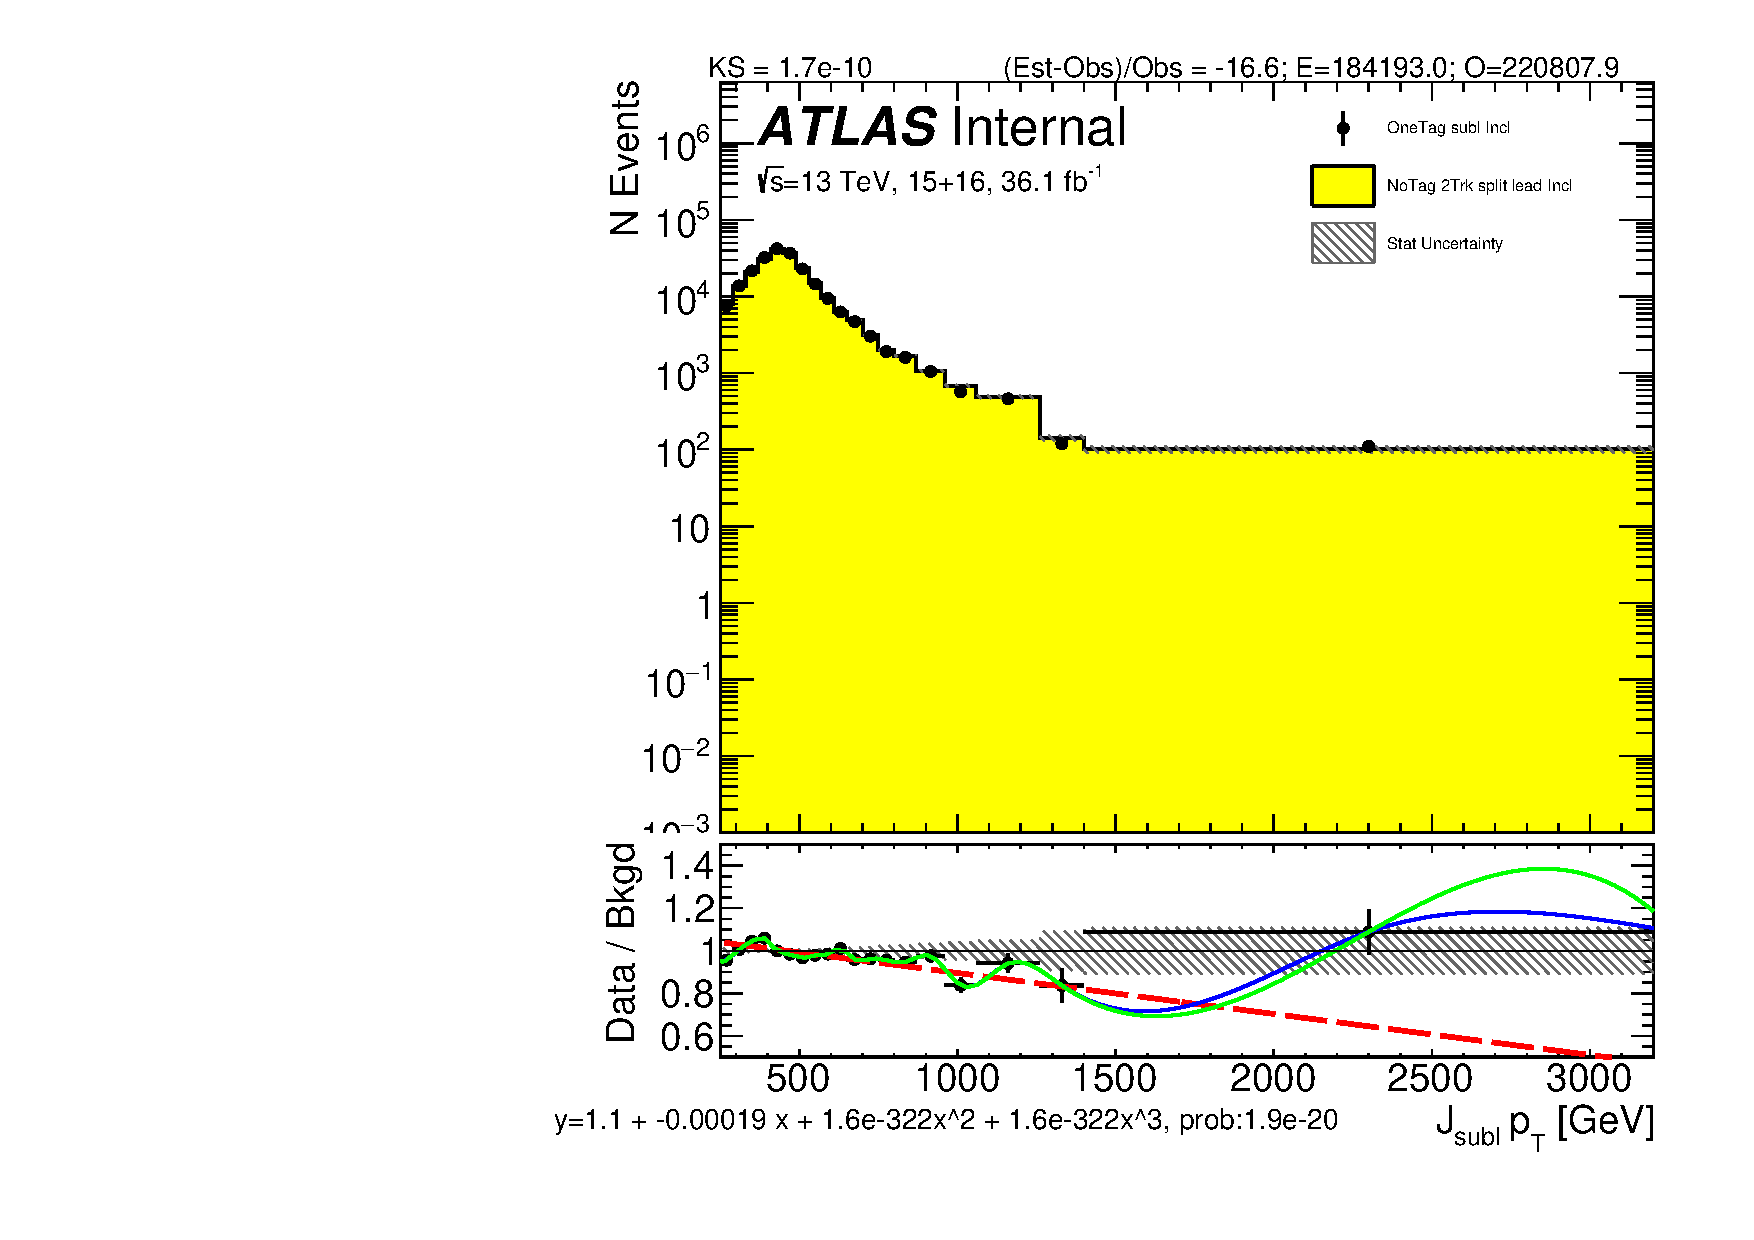
\includegraphics[width=0.32\textwidth,angle=-90]{figures/boosted/Reweight/Fits/Moriond_NoTag_2Trk_split_lead_Incl_sublHCand_Pt_m_1.pdf}
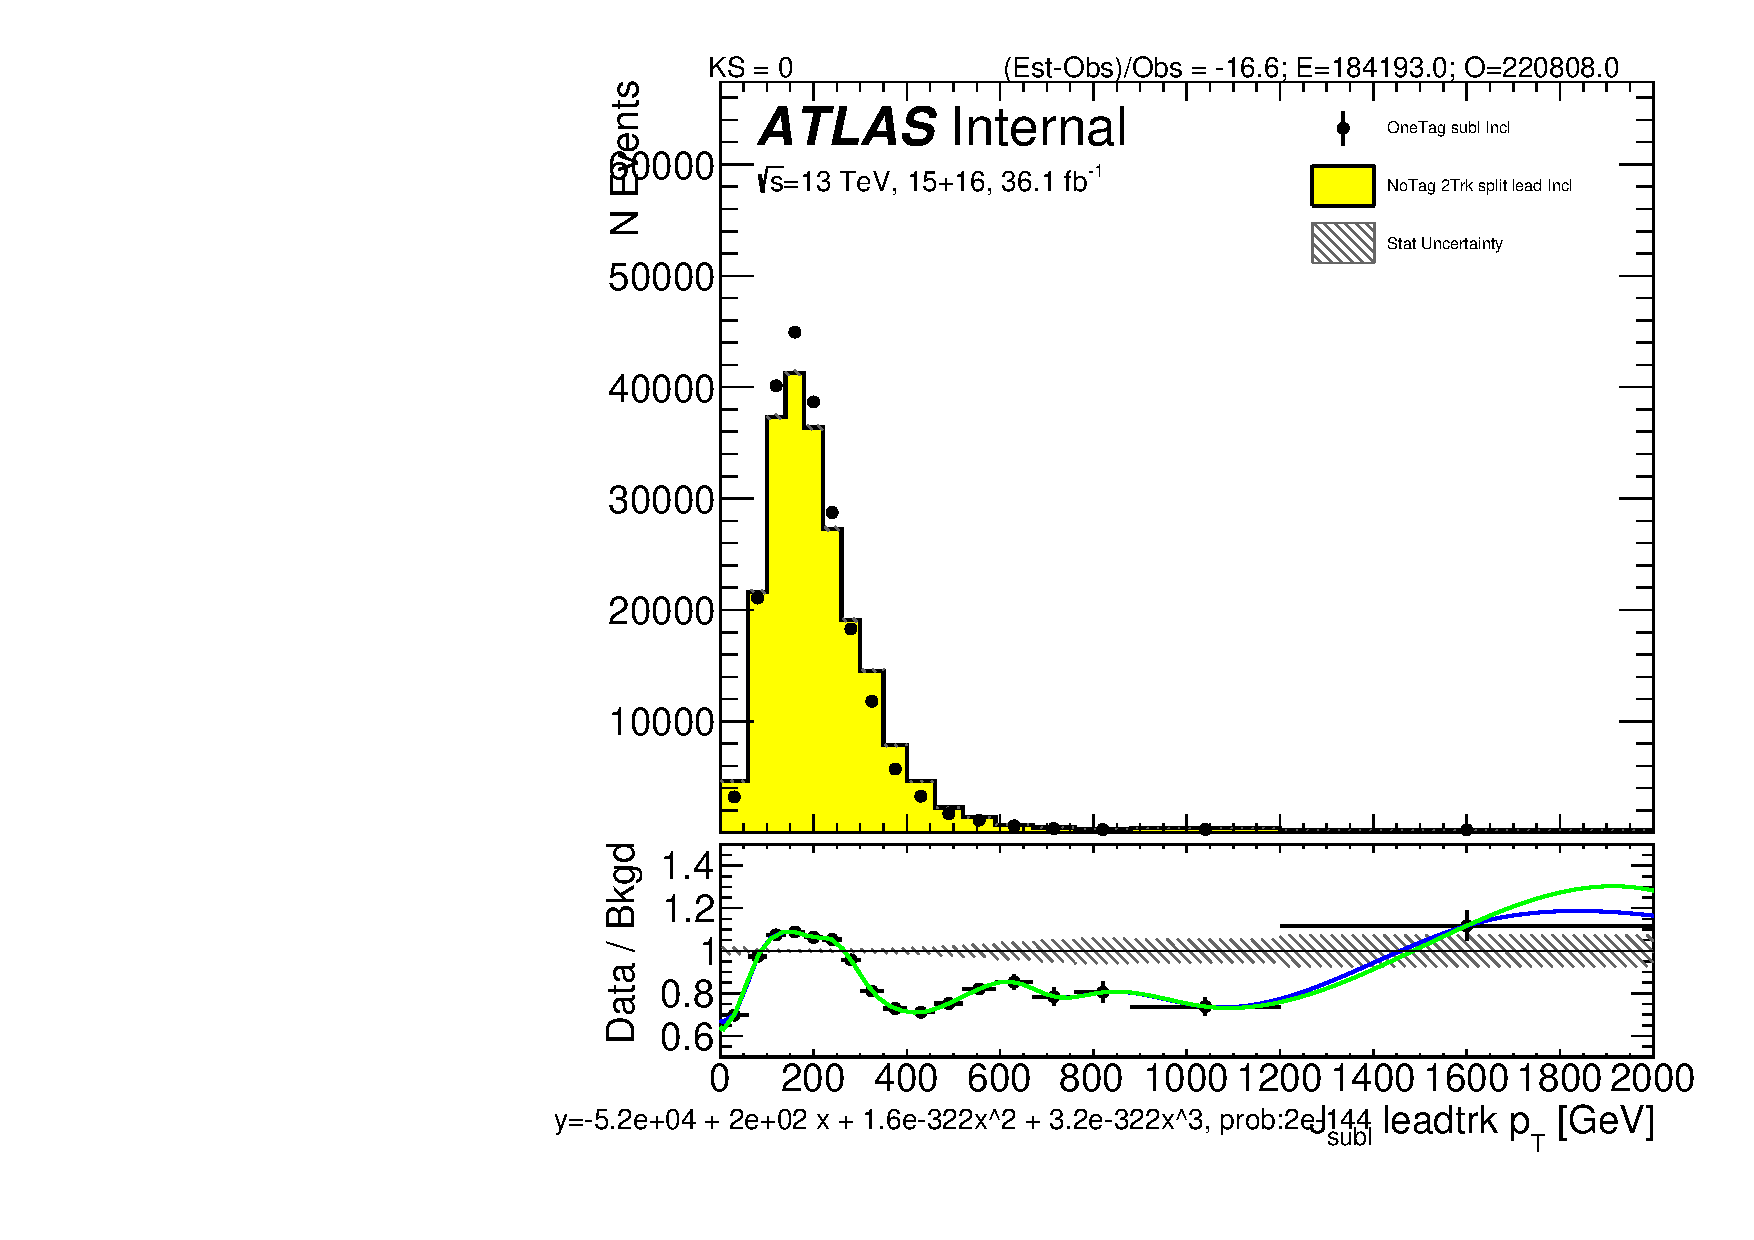
\includegraphics[width=0.32\textwidth,angle=-90]{figures/boosted/Reweight/Fits/Moriond_NoTag_2Trk_split_lead_Incl_sublHCand_trk0_Pt.pdf}
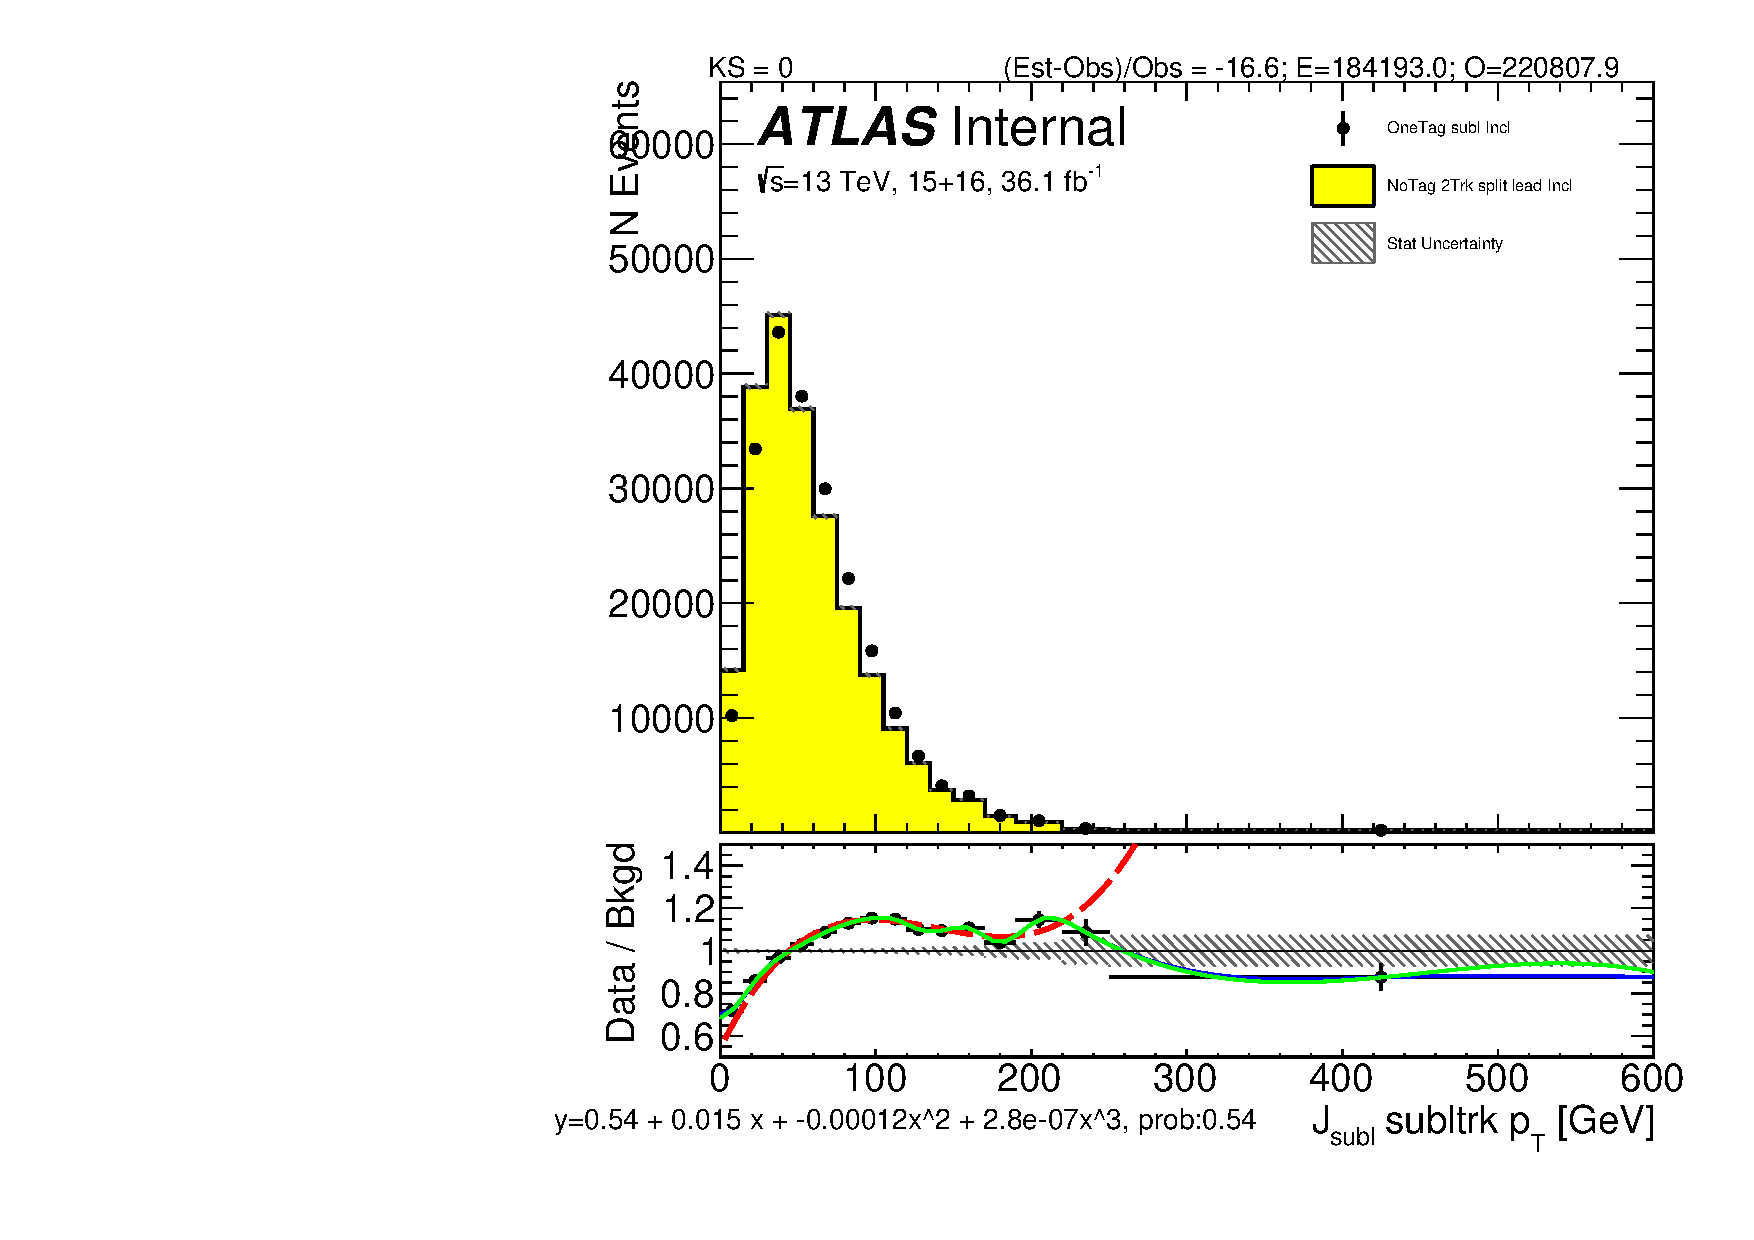
\includegraphics[width=0.32\textwidth,angle=-90]{figures/boosted/Reweight/Fits/Moriond_NoTag_2Trk_split_lead_Incl_sublHCand_trk1_Pt.pdf} \\
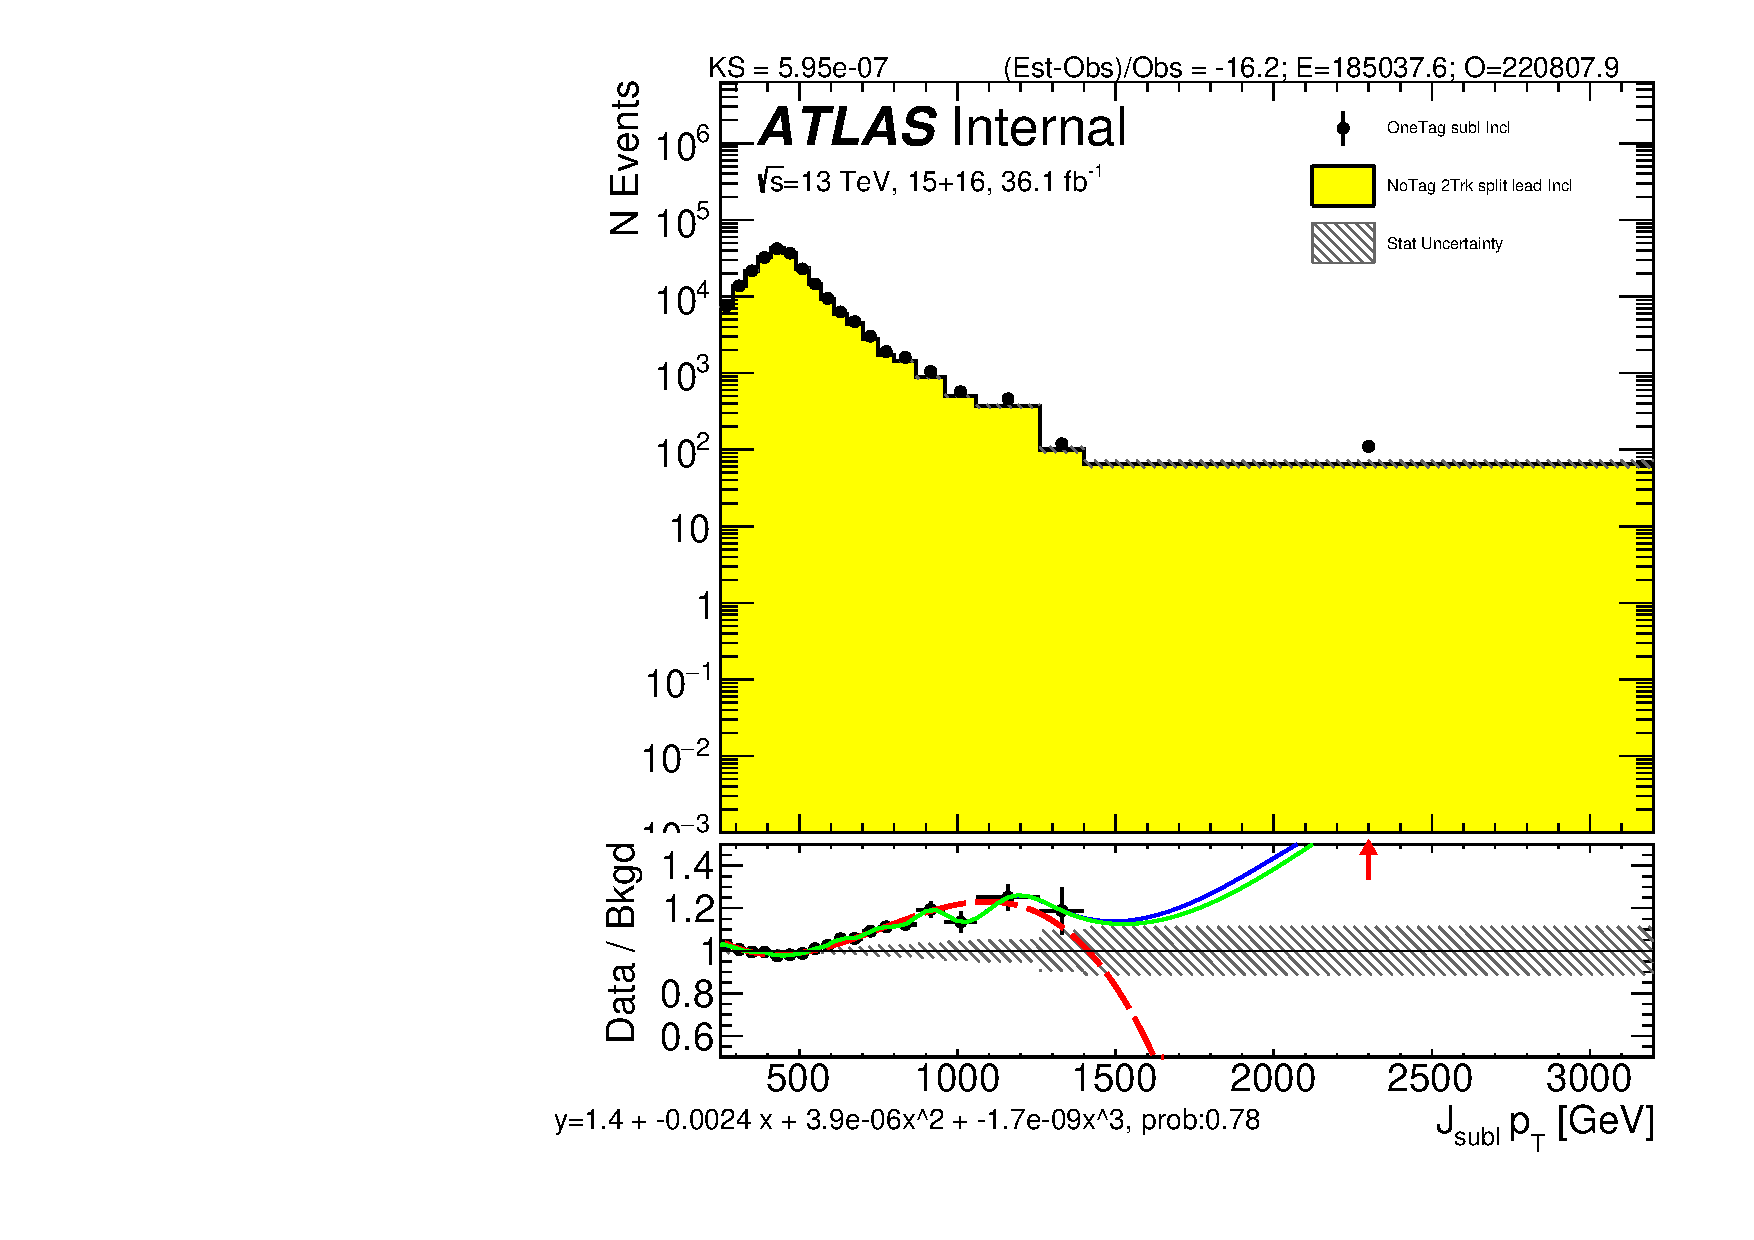
\includegraphics[width=0.32\textwidth,angle=-90]{figures/boosted/Reweight/Fits/Moriond_bkg_0_NoTag_2Trk_split_lead_Incl_sublHCand_Pt_m_1.pdf}
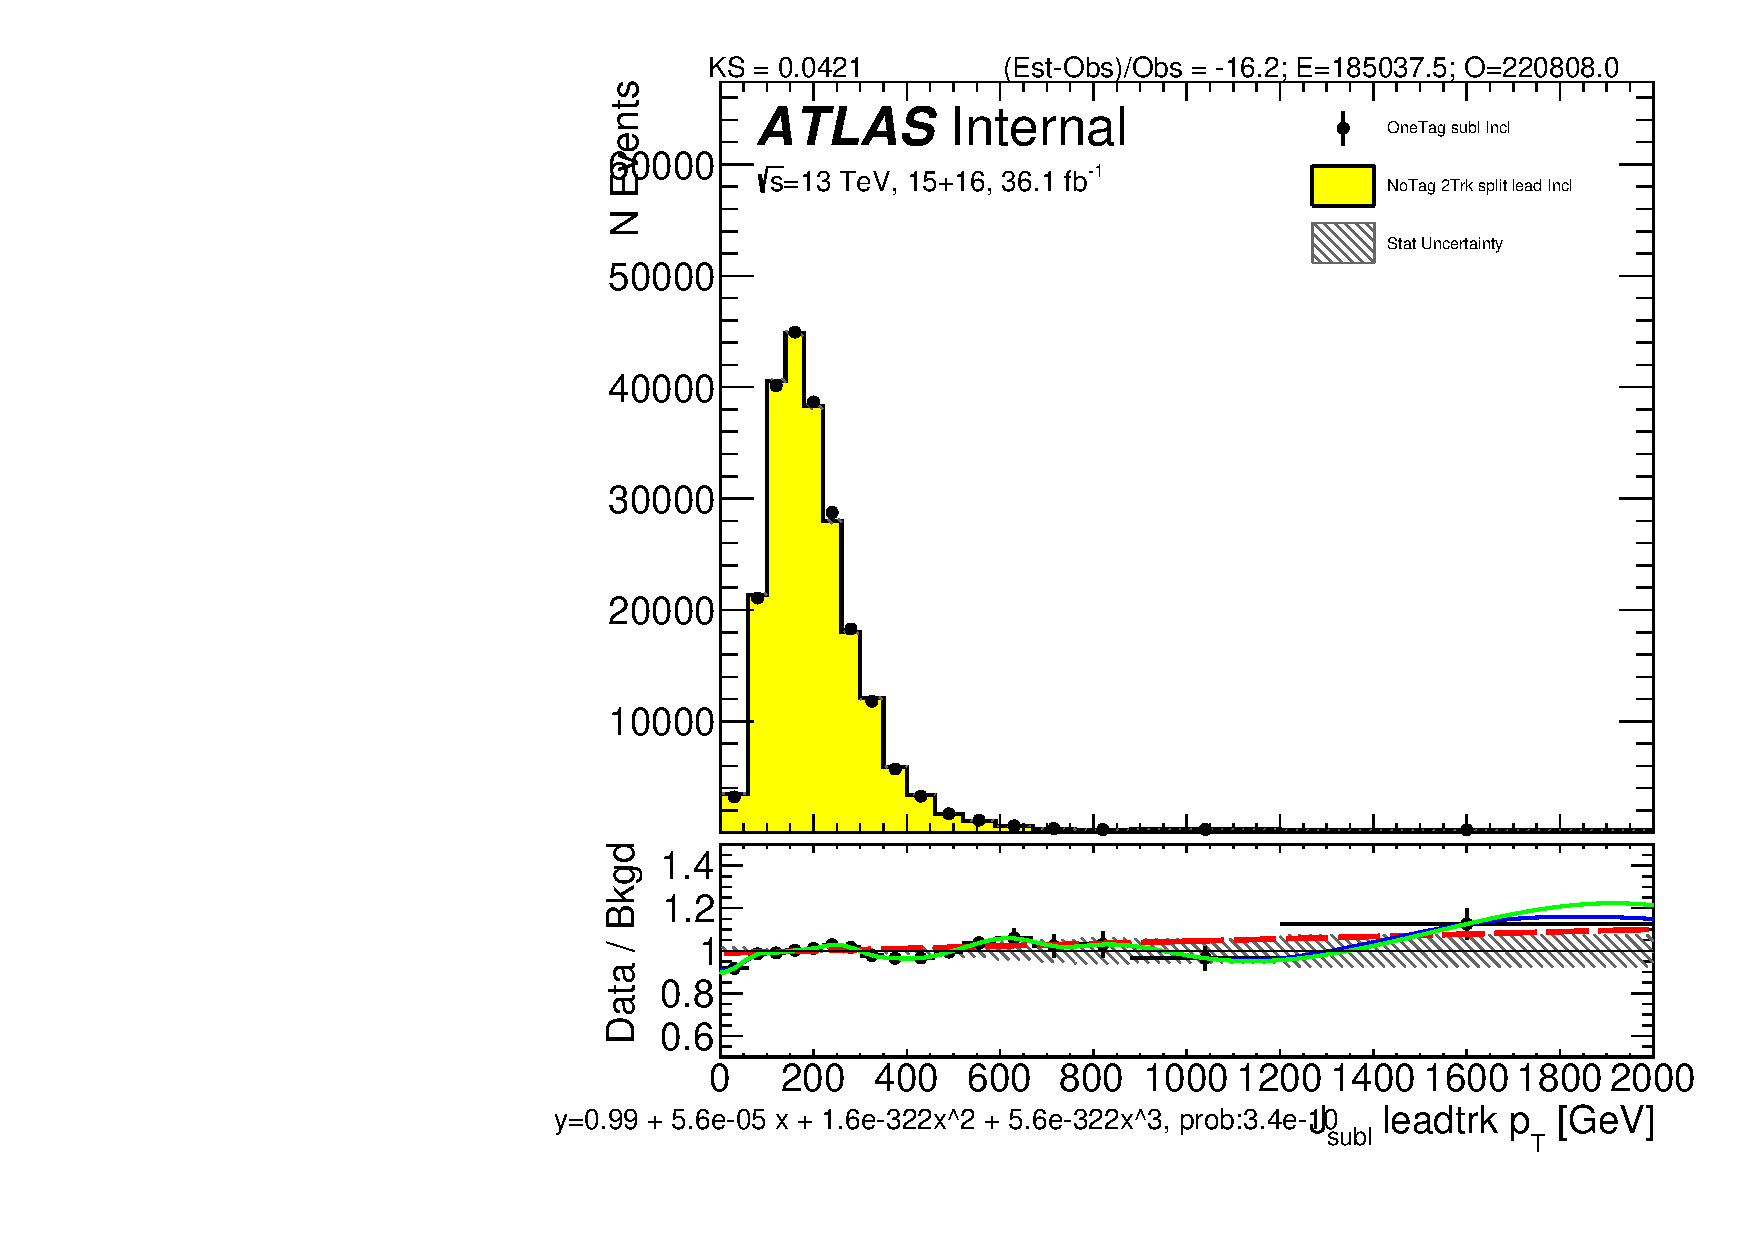
\includegraphics[width=0.32\textwidth,angle=-90]{figures/boosted/Reweight/Fits/Moriond_bkg_0_NoTag_2Trk_split_lead_Incl_sublHCand_trk0_Pt.pdf}
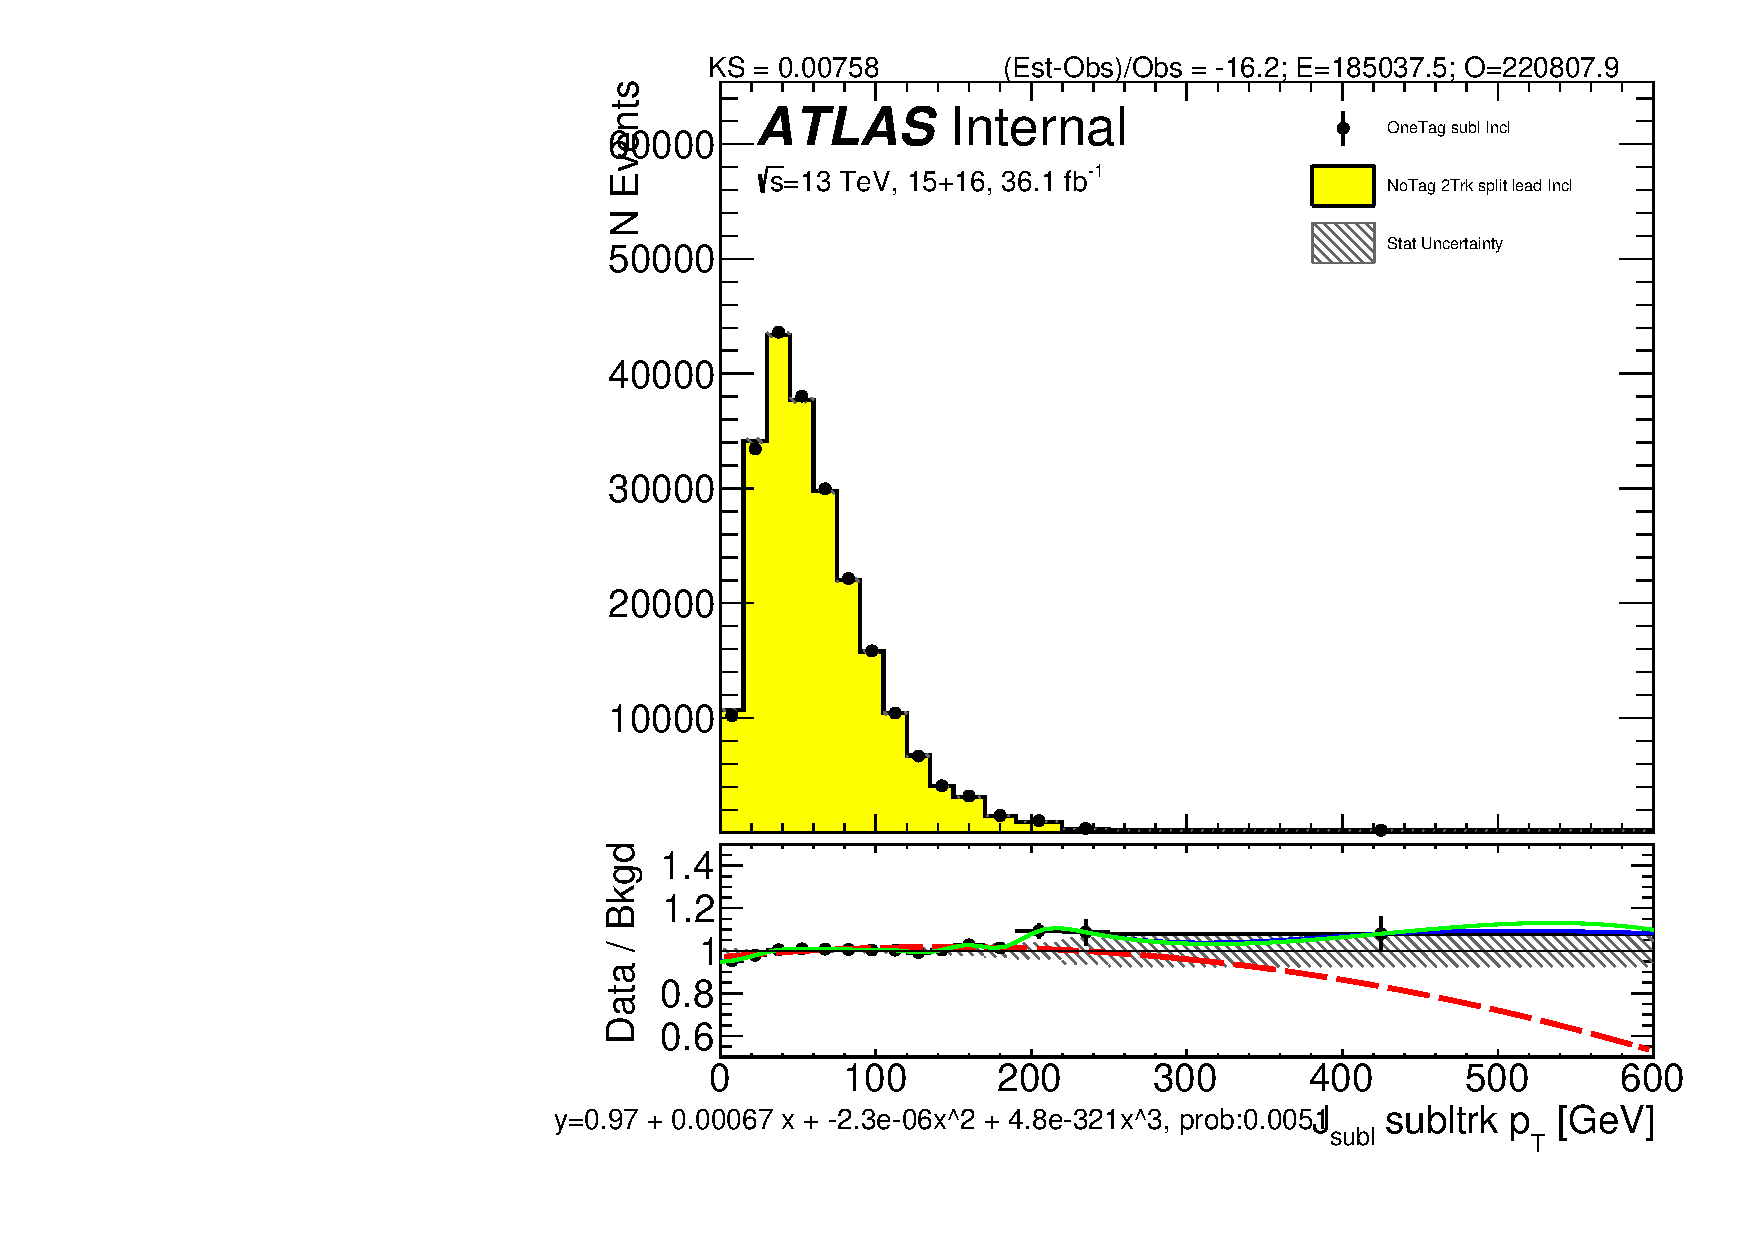
\includegraphics[width=0.32\textwidth,angle=-90]{figures/boosted/Reweight/Fits/Moriond_bkg_0_NoTag_2Trk_split_lead_Incl_sublHCand_trk1_Pt.pdf} \\
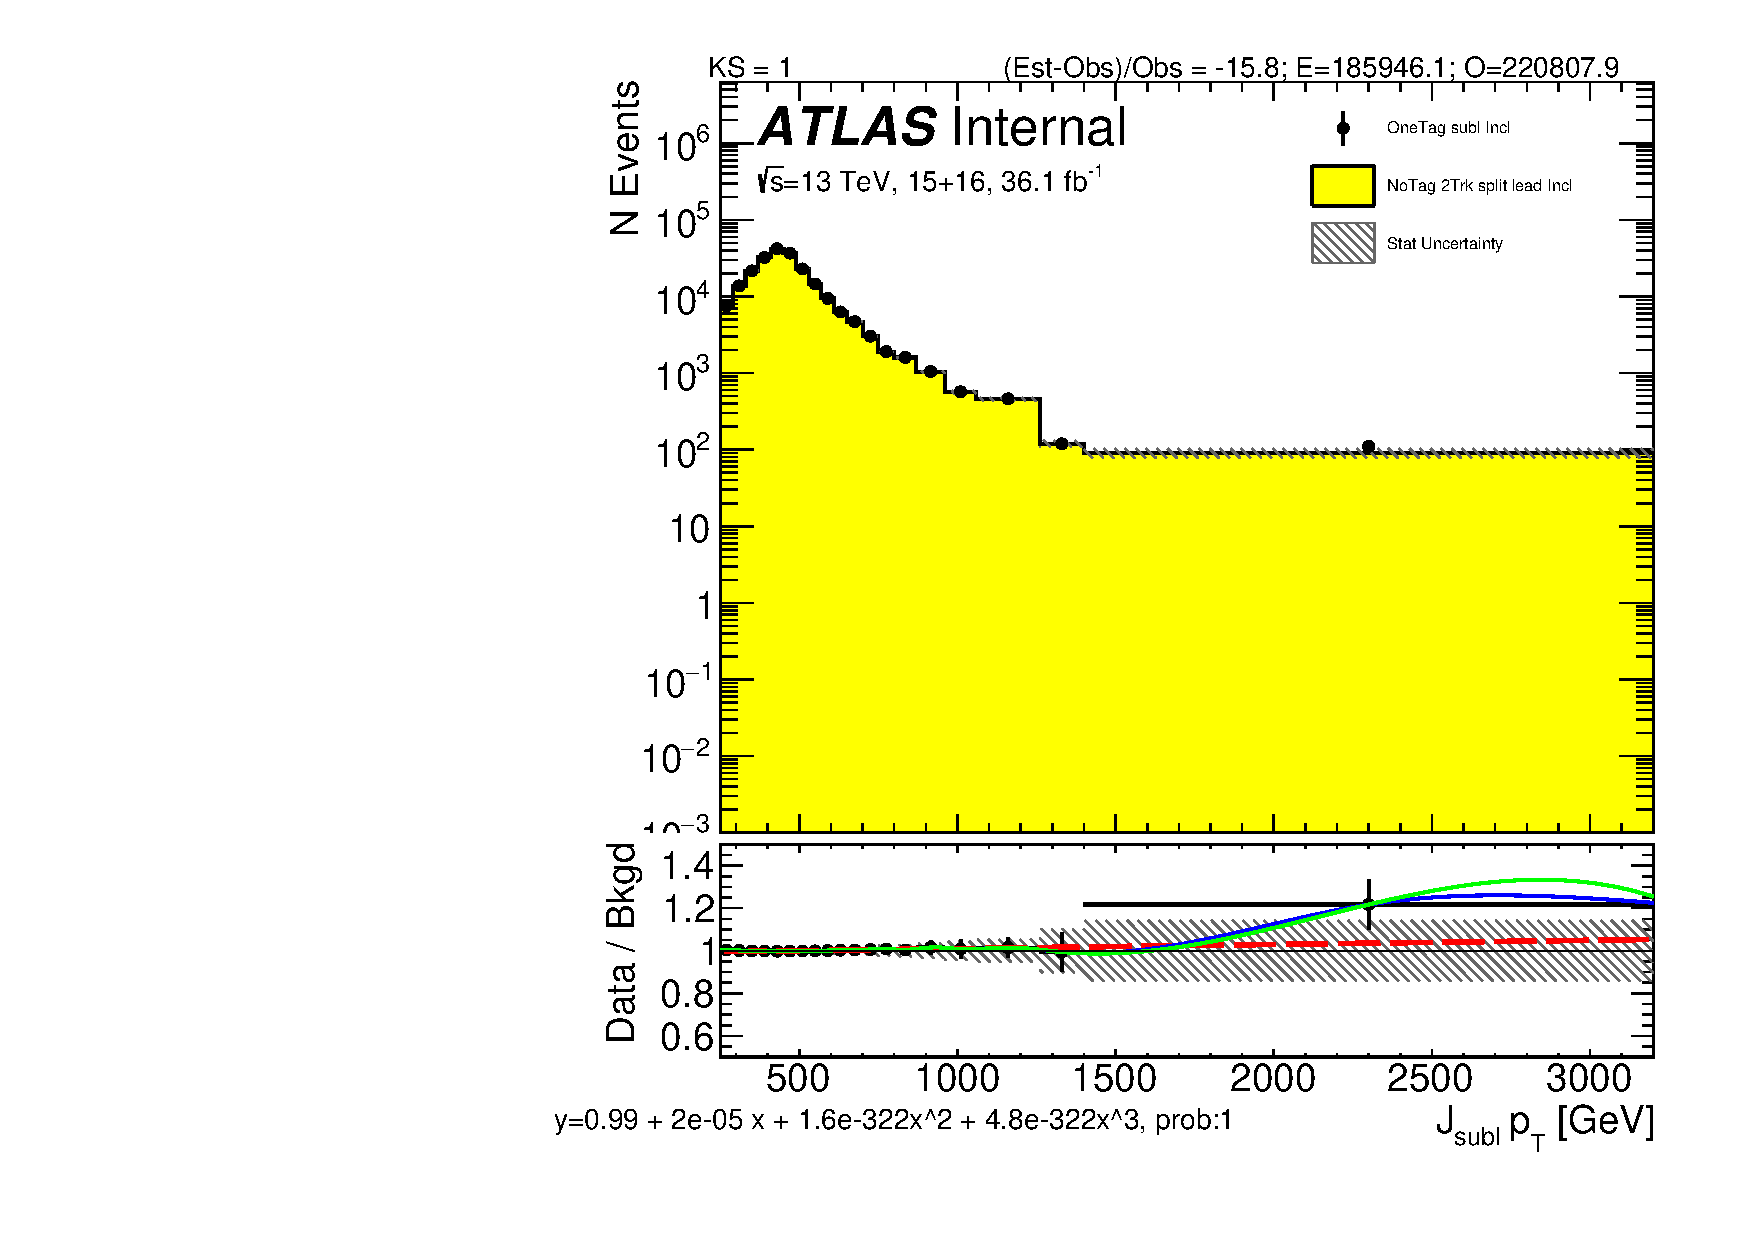
\includegraphics[width=0.32\textwidth,angle=-90]{figures/boosted/Reweight/Fits/Moriond_bkg_3_NoTag_2Trk_split_lead_Incl_sublHCand_Pt_m_1.pdf}
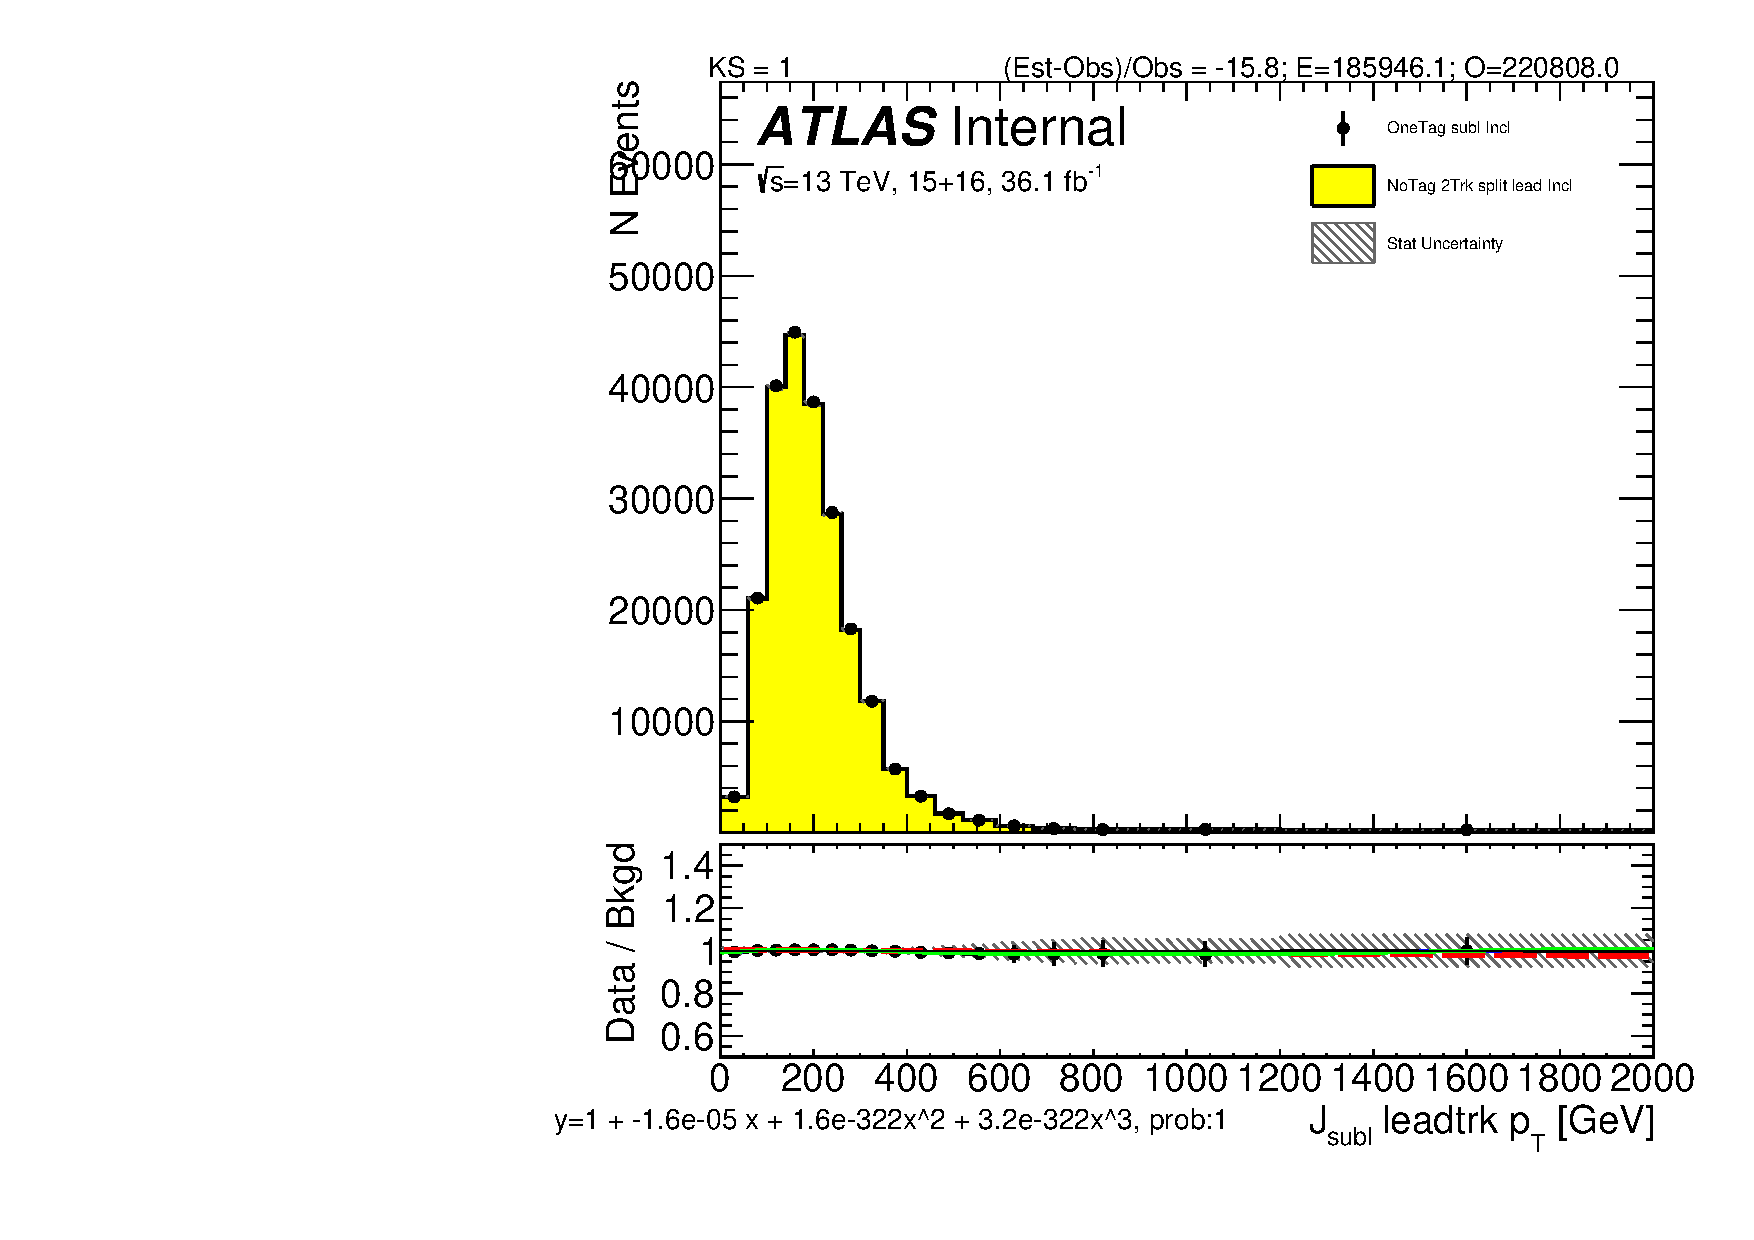
\includegraphics[width=0.32\textwidth,angle=-90]{figures/boosted/Reweight/Fits/Moriond_bkg_3_NoTag_2Trk_split_lead_Incl_sublHCand_trk0_Pt.pdf}
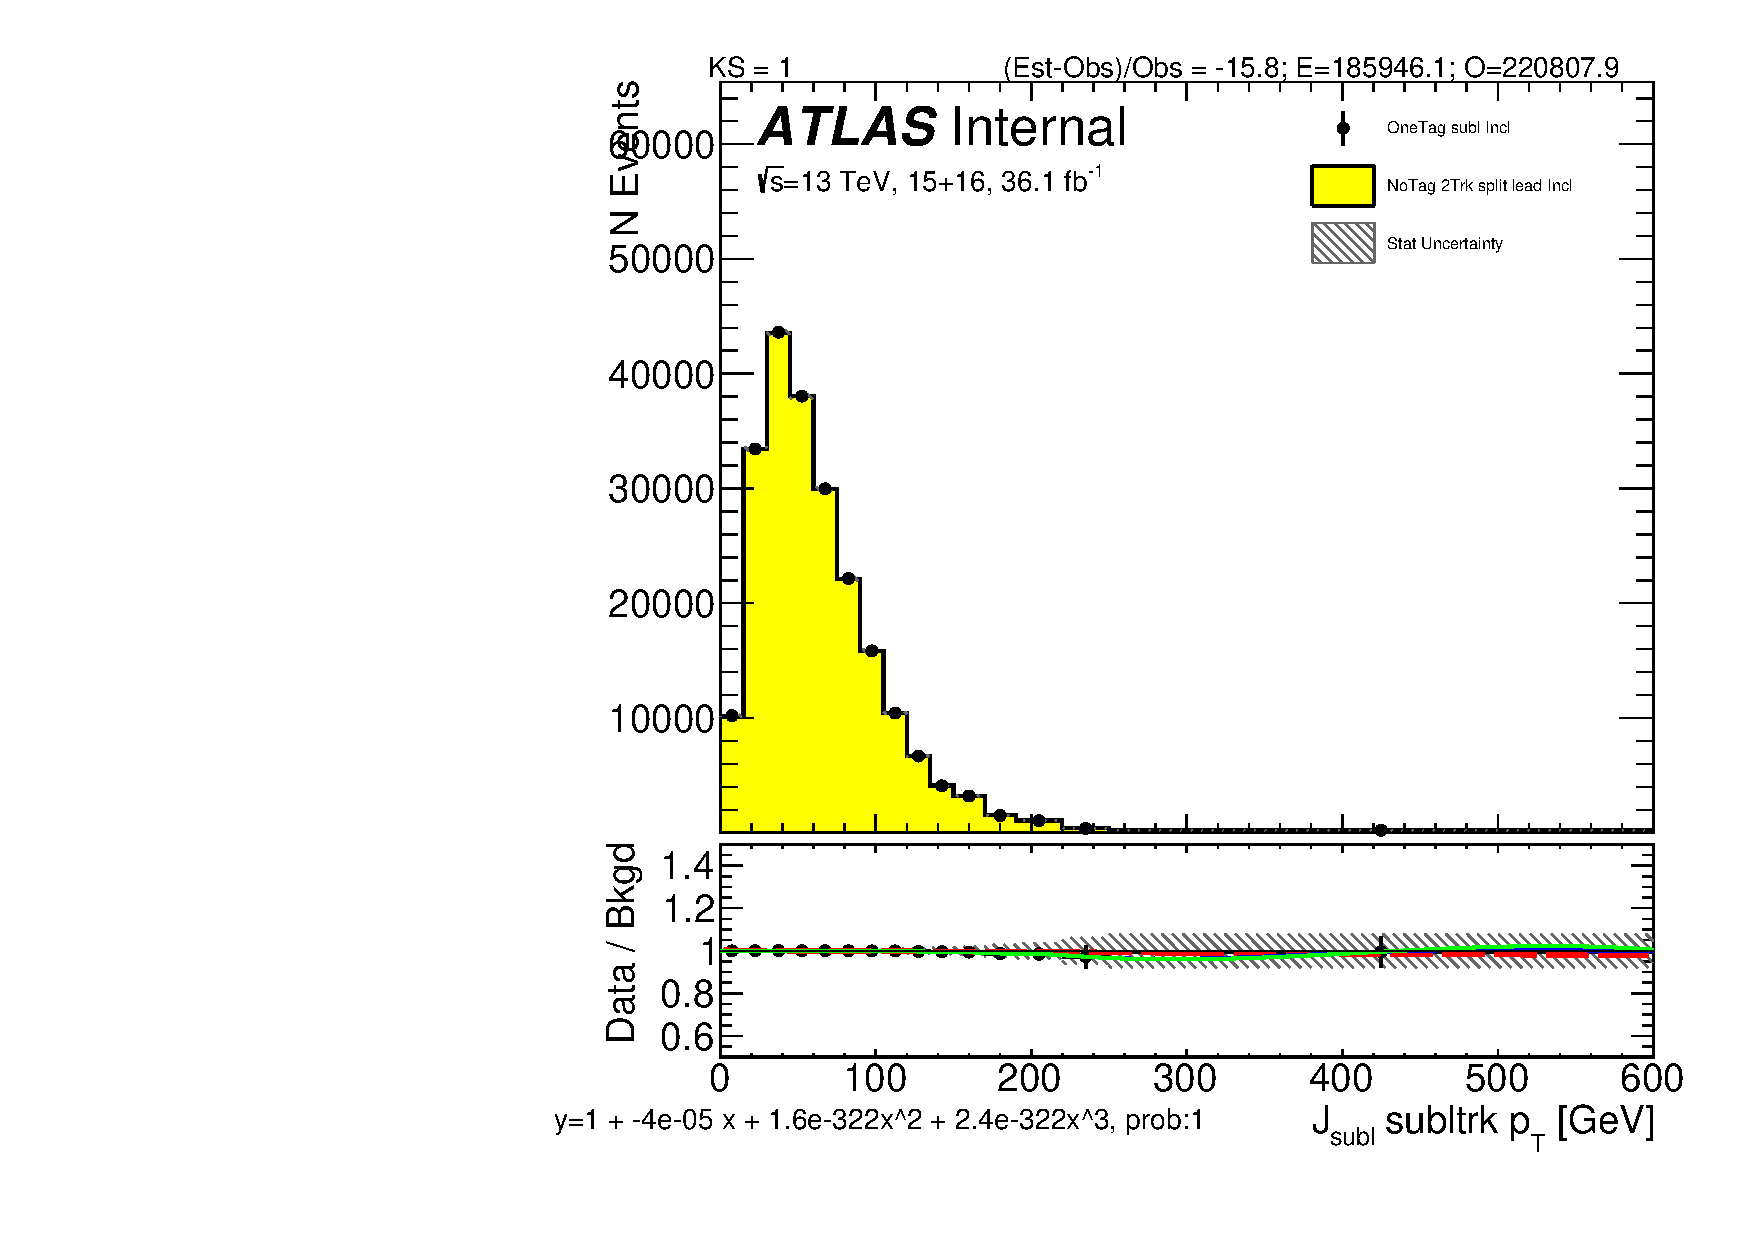
\includegraphics[width=0.32\textwidth,angle=-90]{figures/boosted/Reweight/Fits/Moriond_bkg_3_NoTag_2Trk_split_lead_Incl_sublHCand_trk1_Pt.pdf} \\
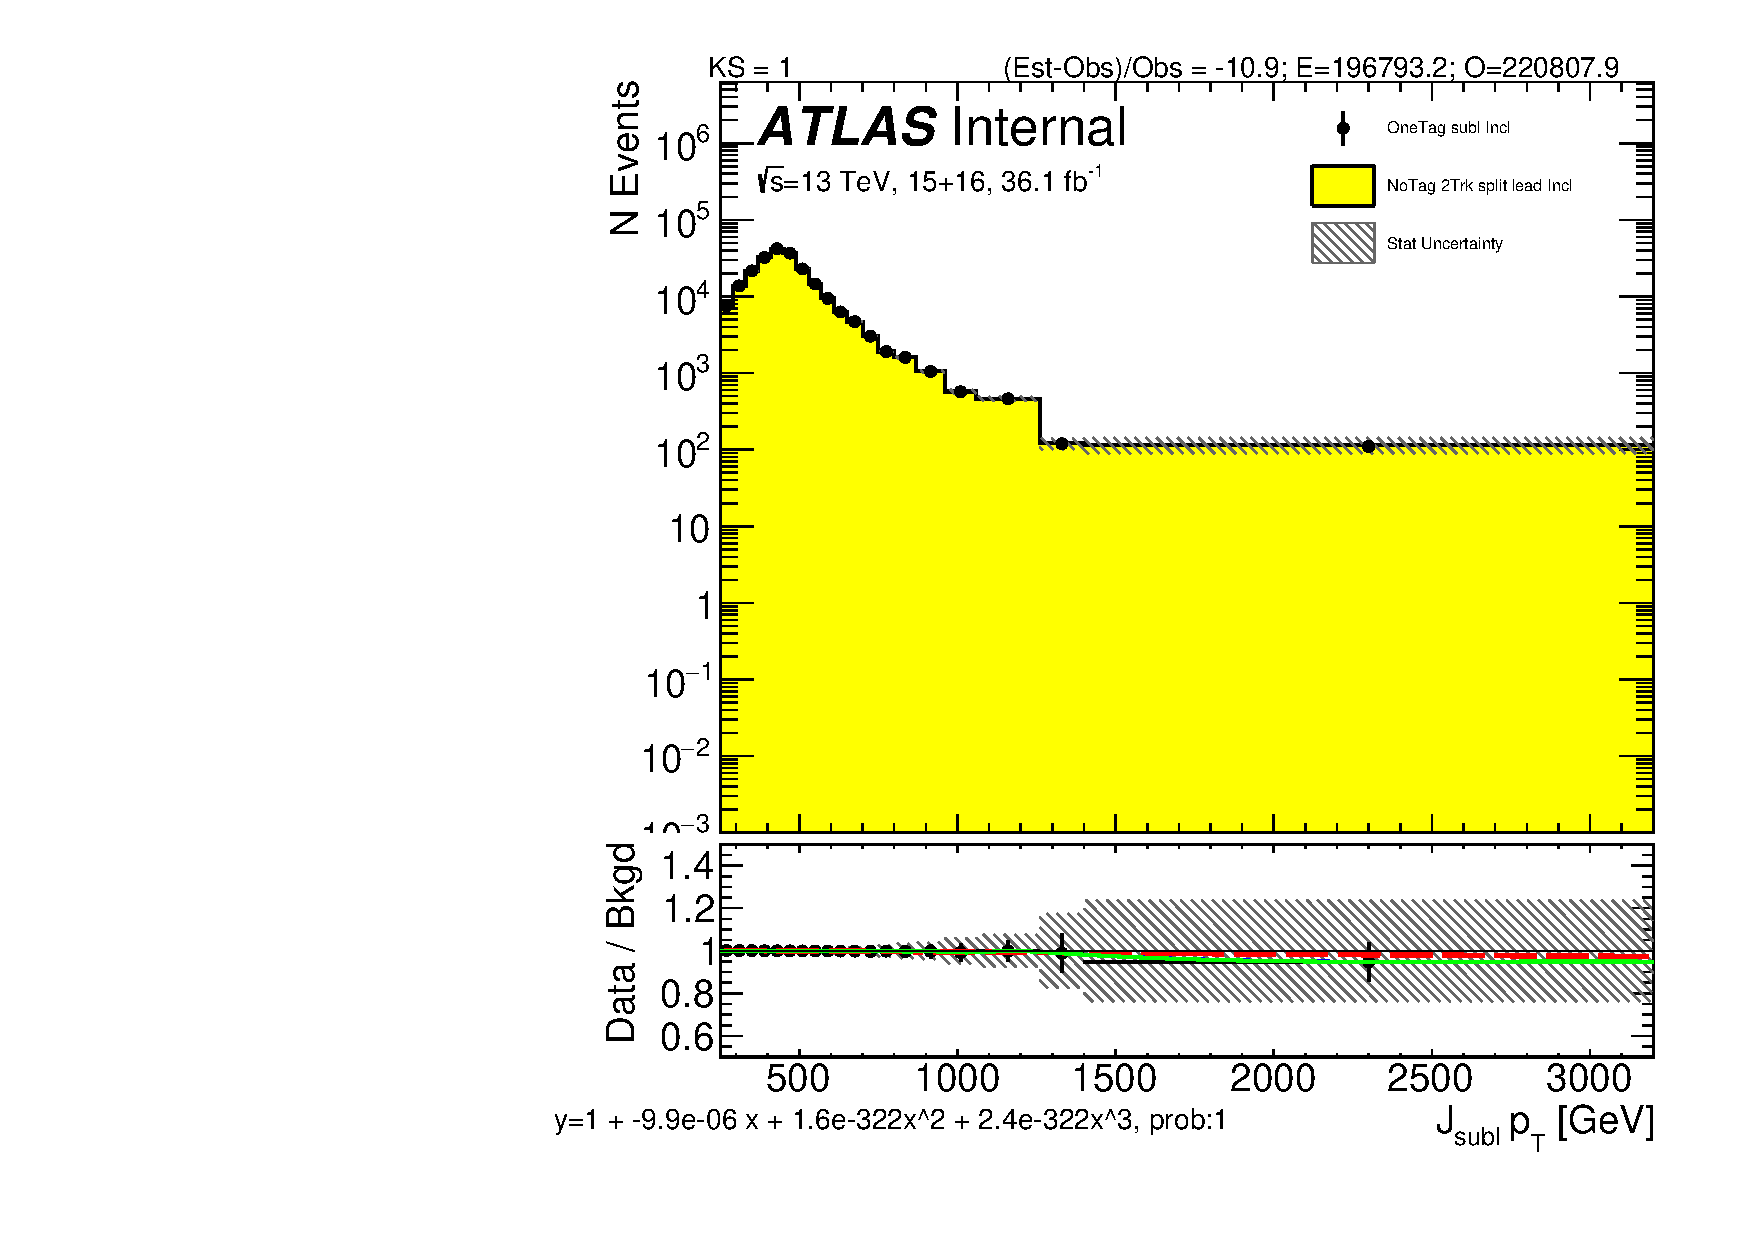
\includegraphics[width=0.32\textwidth,angle=-90]{figures/boosted/Reweight/Fits/Moriond_bkg_9_NoTag_2Trk_split_lead_Incl_sublHCand_Pt_m_1.pdf}
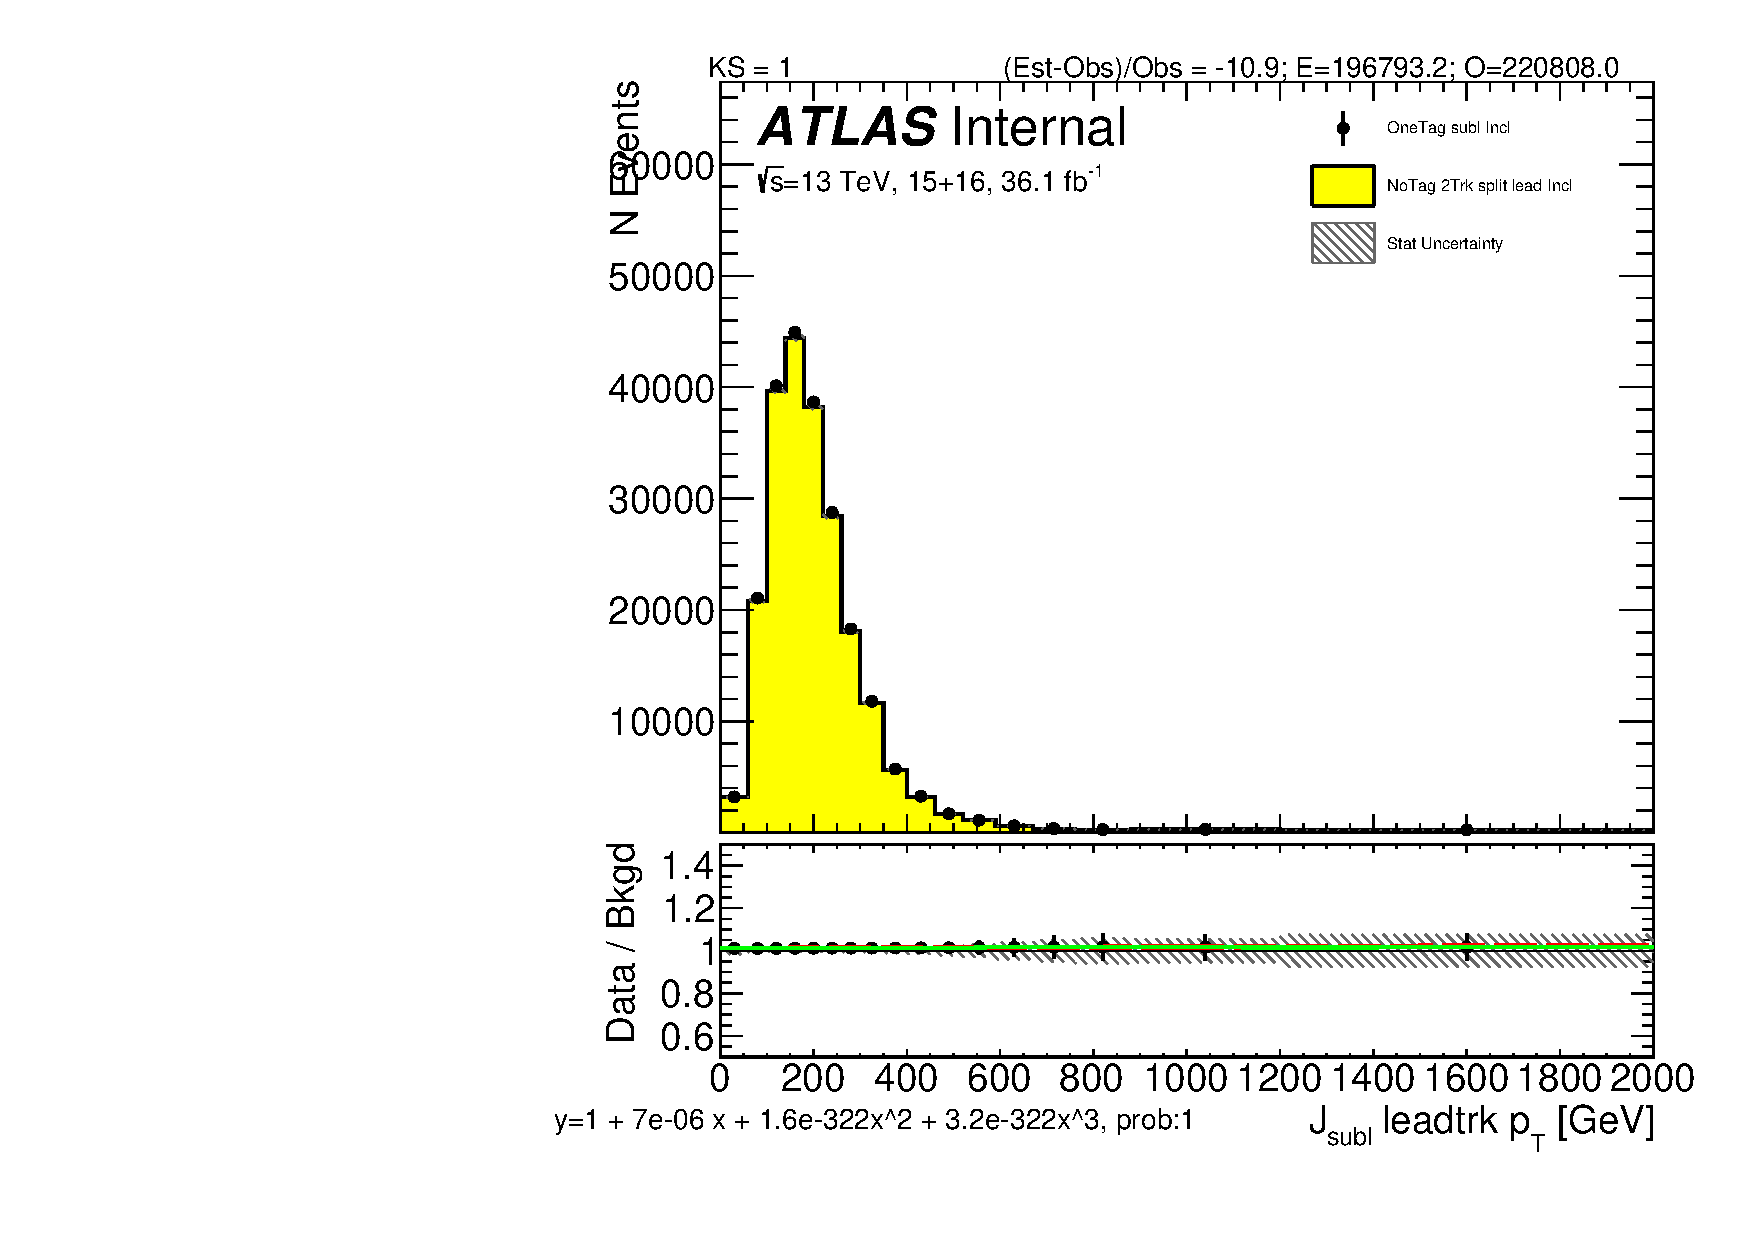
\includegraphics[width=0.32\textwidth,angle=-90]{figures/boosted/Reweight/Fits/Moriond_bkg_9_NoTag_2Trk_split_lead_Incl_sublHCand_trk0_Pt.pdf}
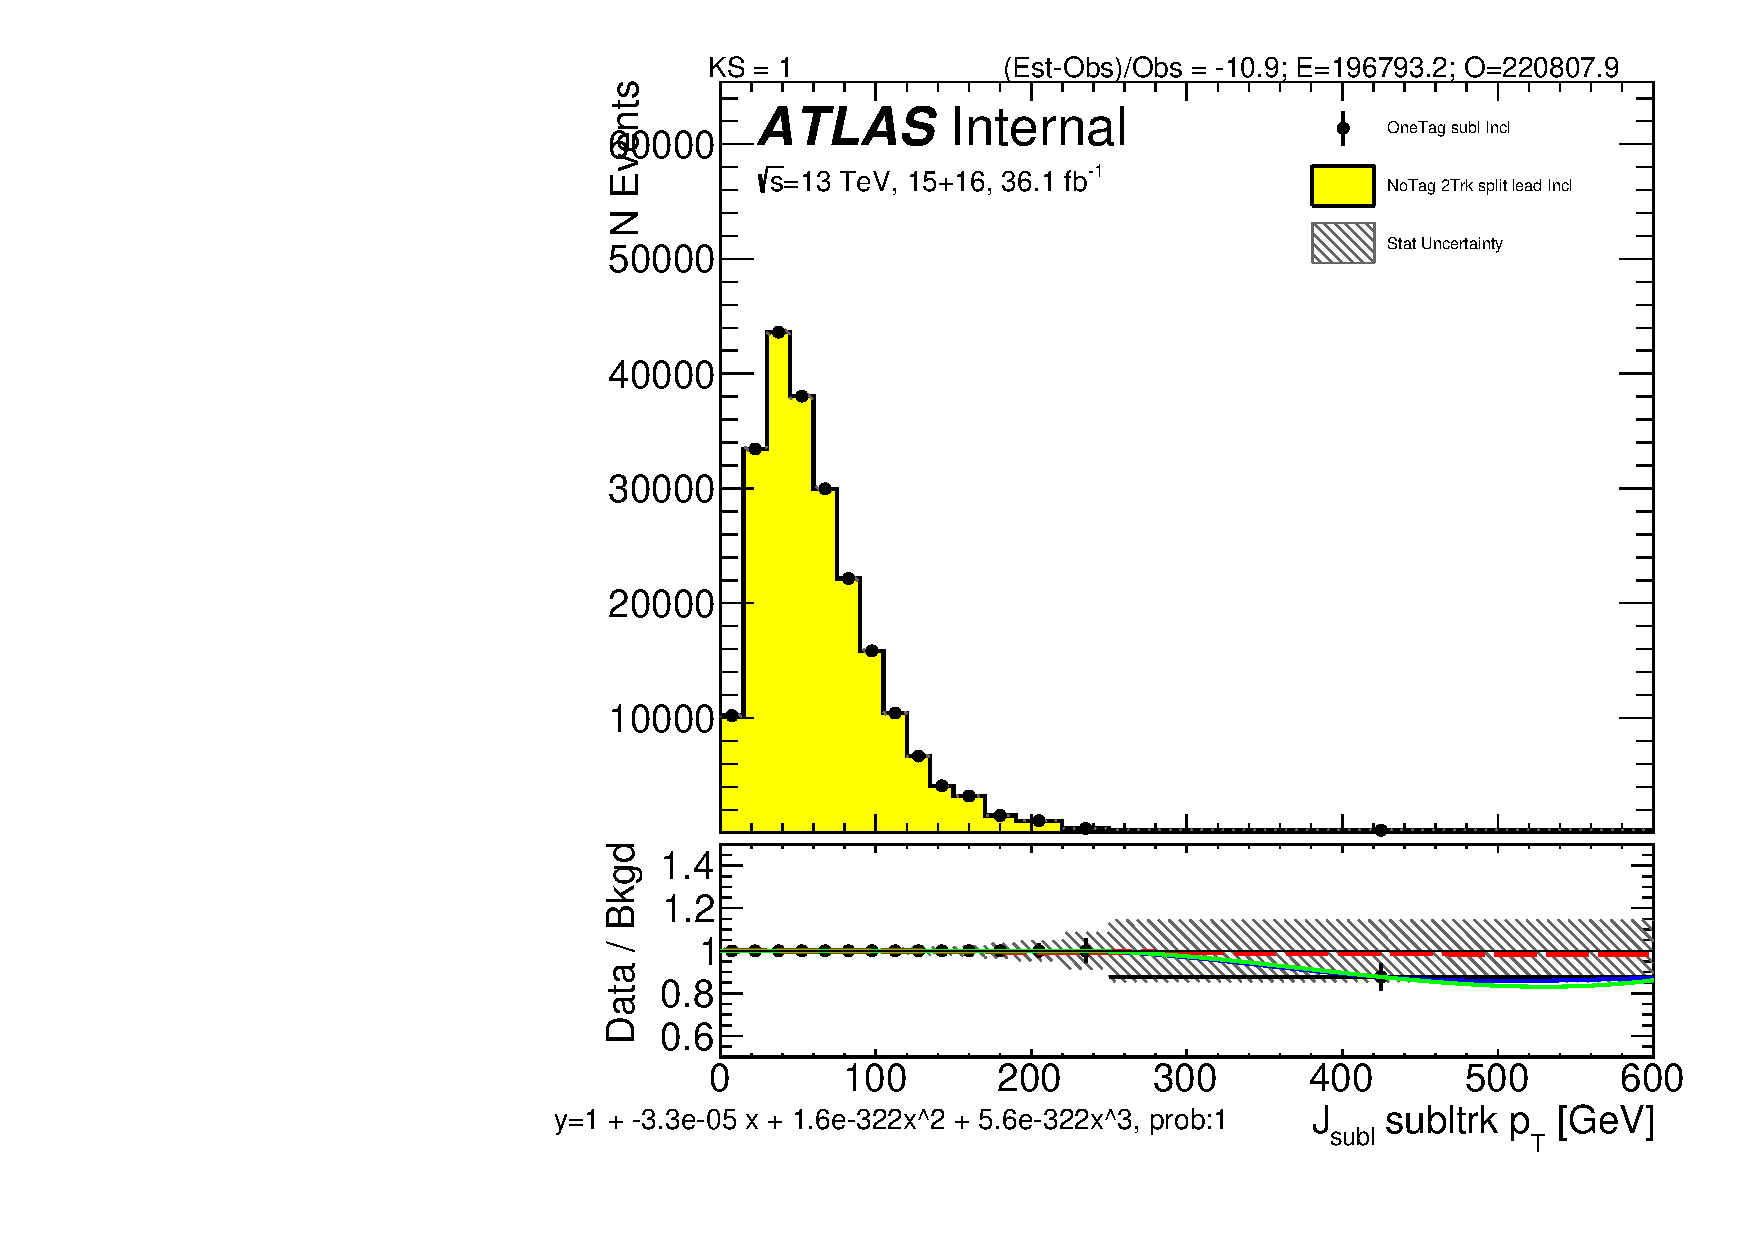
\includegraphics[width=0.32\textwidth,angle=-90]{figures/boosted/Reweight/Fits/Moriond_bkg_9_NoTag_2Trk_split_lead_Incl_sublHCand_trk1_Pt.pdf} \\
\caption{For $2bs$ background estimate: the fits to the ratio of the data in the $1b$ category, of the sublleading Higgs candidate $1b$-tagged events's subleading Higgs candidate distributions(black point), over the leading Higgs candidate $1b$-tagged events's subleading Higgs candidate distributions(yellow). Distributions and fits to the estimated QCD background for large-$R$ jet $p_{T}$ (left),  the large-$R$ jet's leading trackjet $p_T$ (middle), and large-$R$ jet's subleading trackjet $p_T$ (right) are shown.  Figure are shown before reweighting (top row), after the first iteration(second row), after the fourth iteration(third row), and after the last iteration (bottow row). The green line is the spline extrapolation; and the red line is a polynomial fit.}
\label{fig:rw-2bs-lead}
\end{center}
\end{figure*}

\begin{figure*}[htbp!]
\begin{center}
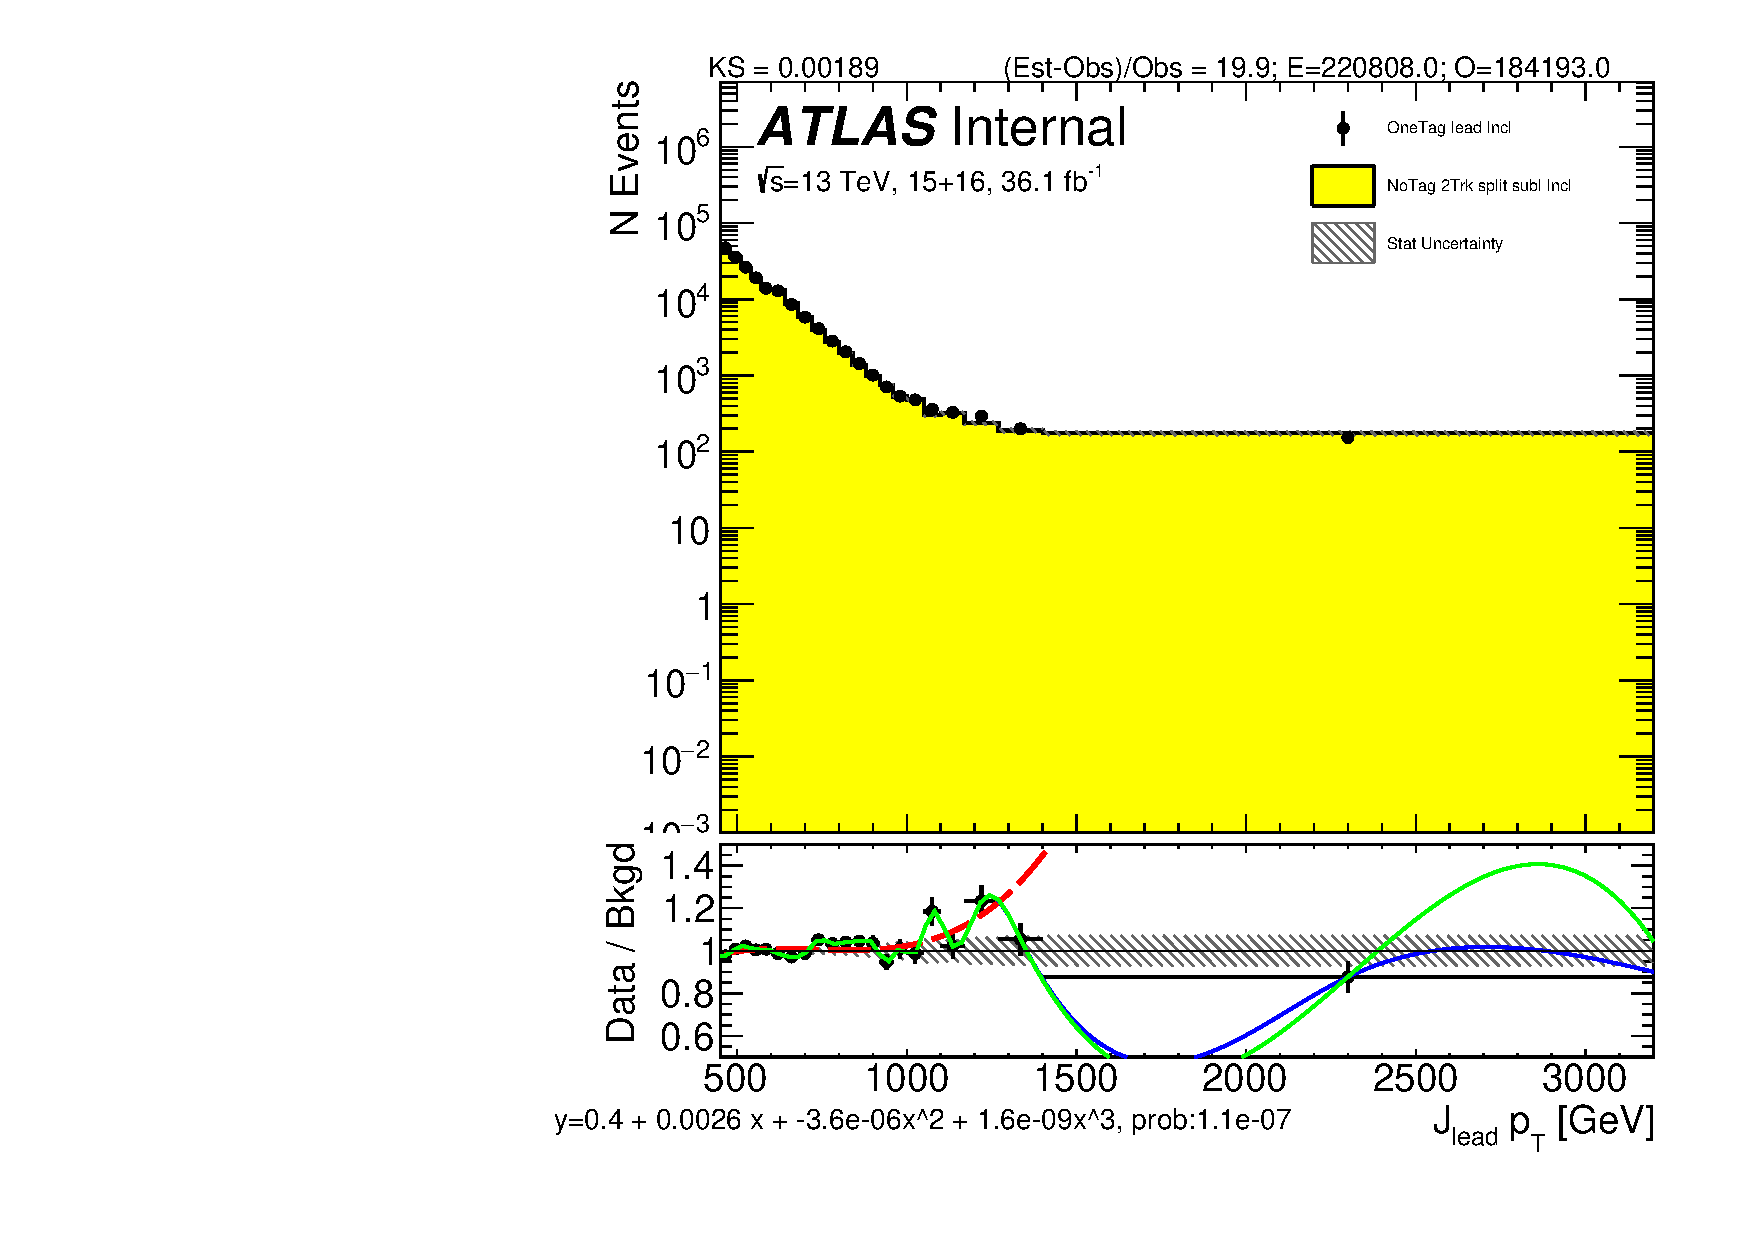
\includegraphics[width=0.32\textwidth,angle=-90]{figures/boosted/Reweight/Fits/Moriond_NoTag_2Trk_split_subl_Incl_leadHCand_Pt_m_1.pdf}
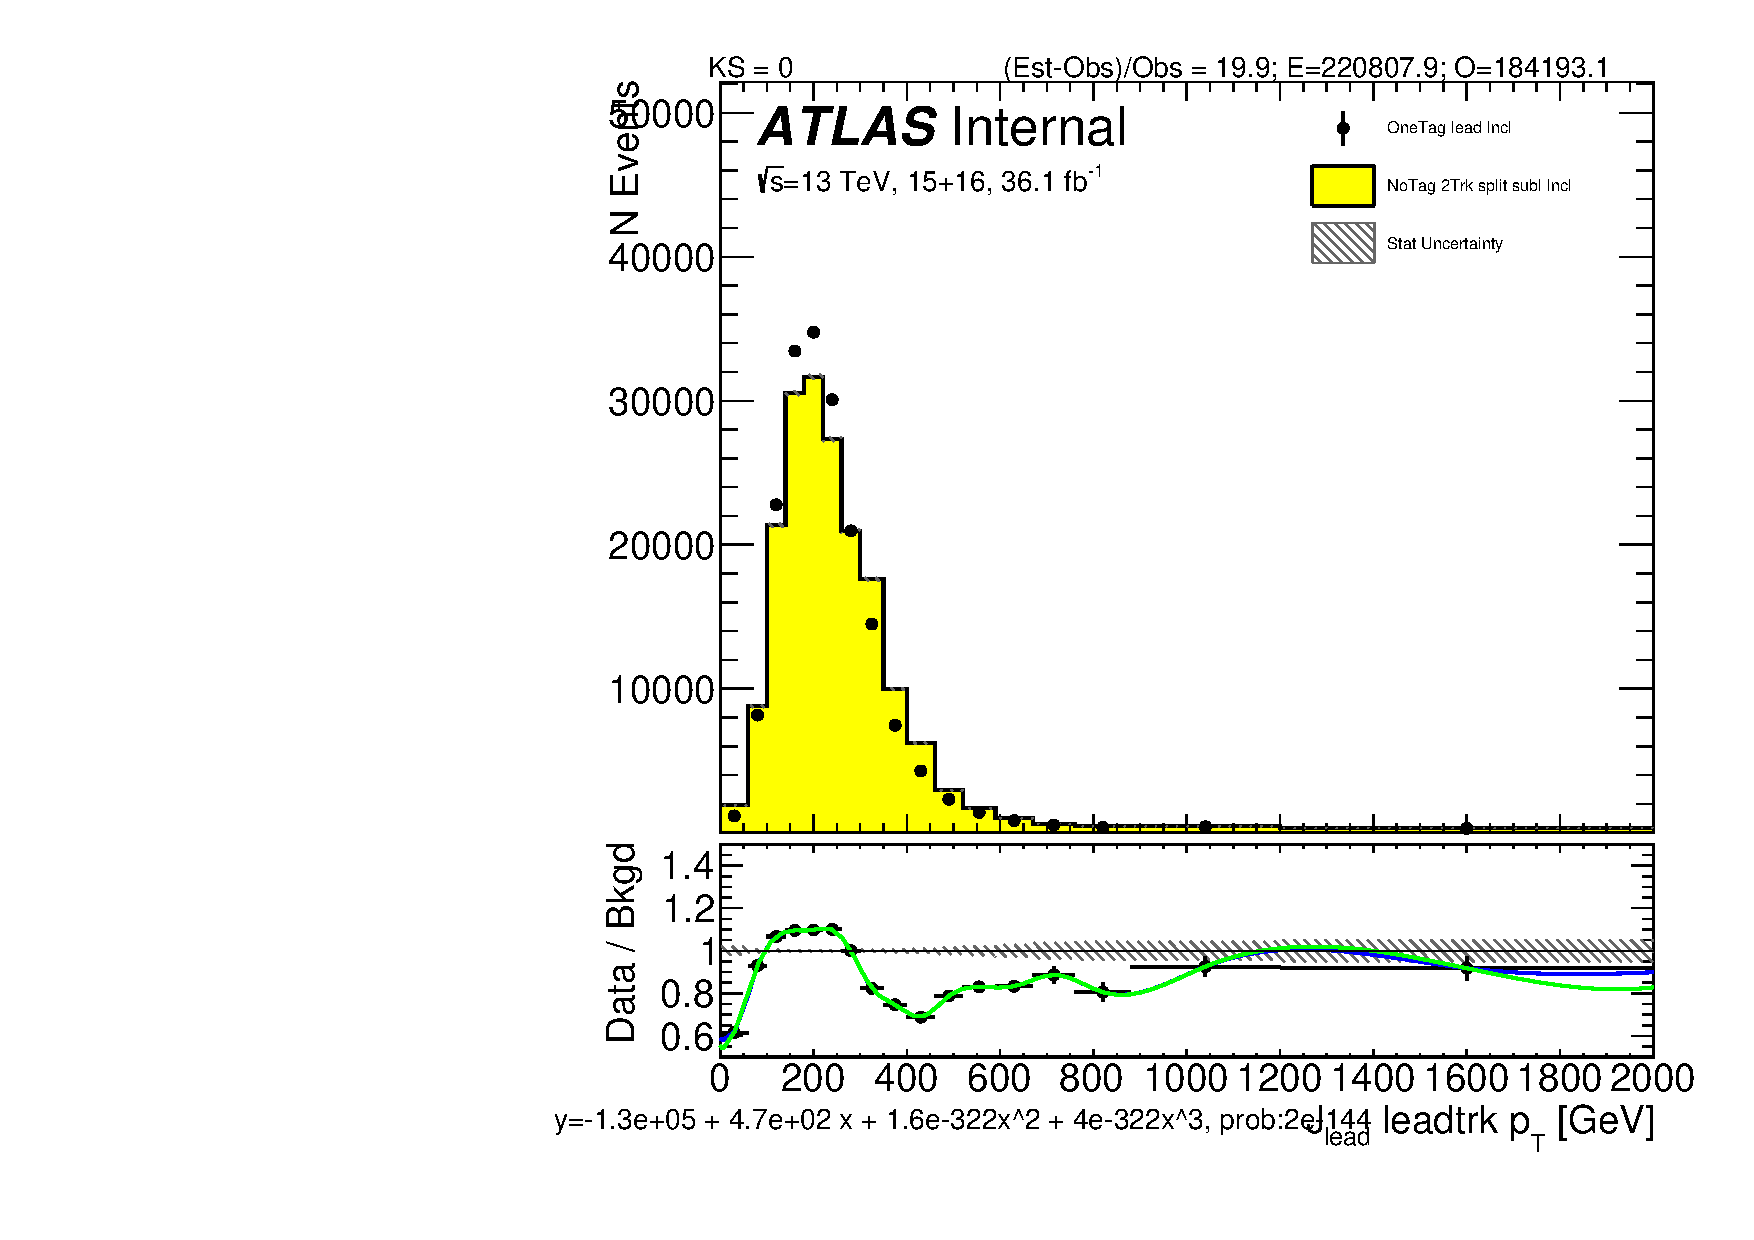
\includegraphics[width=0.32\textwidth,angle=-90]{figures/boosted/Reweight/Fits/Moriond_NoTag_2Trk_split_subl_Incl_leadHCand_trk0_Pt.pdf}
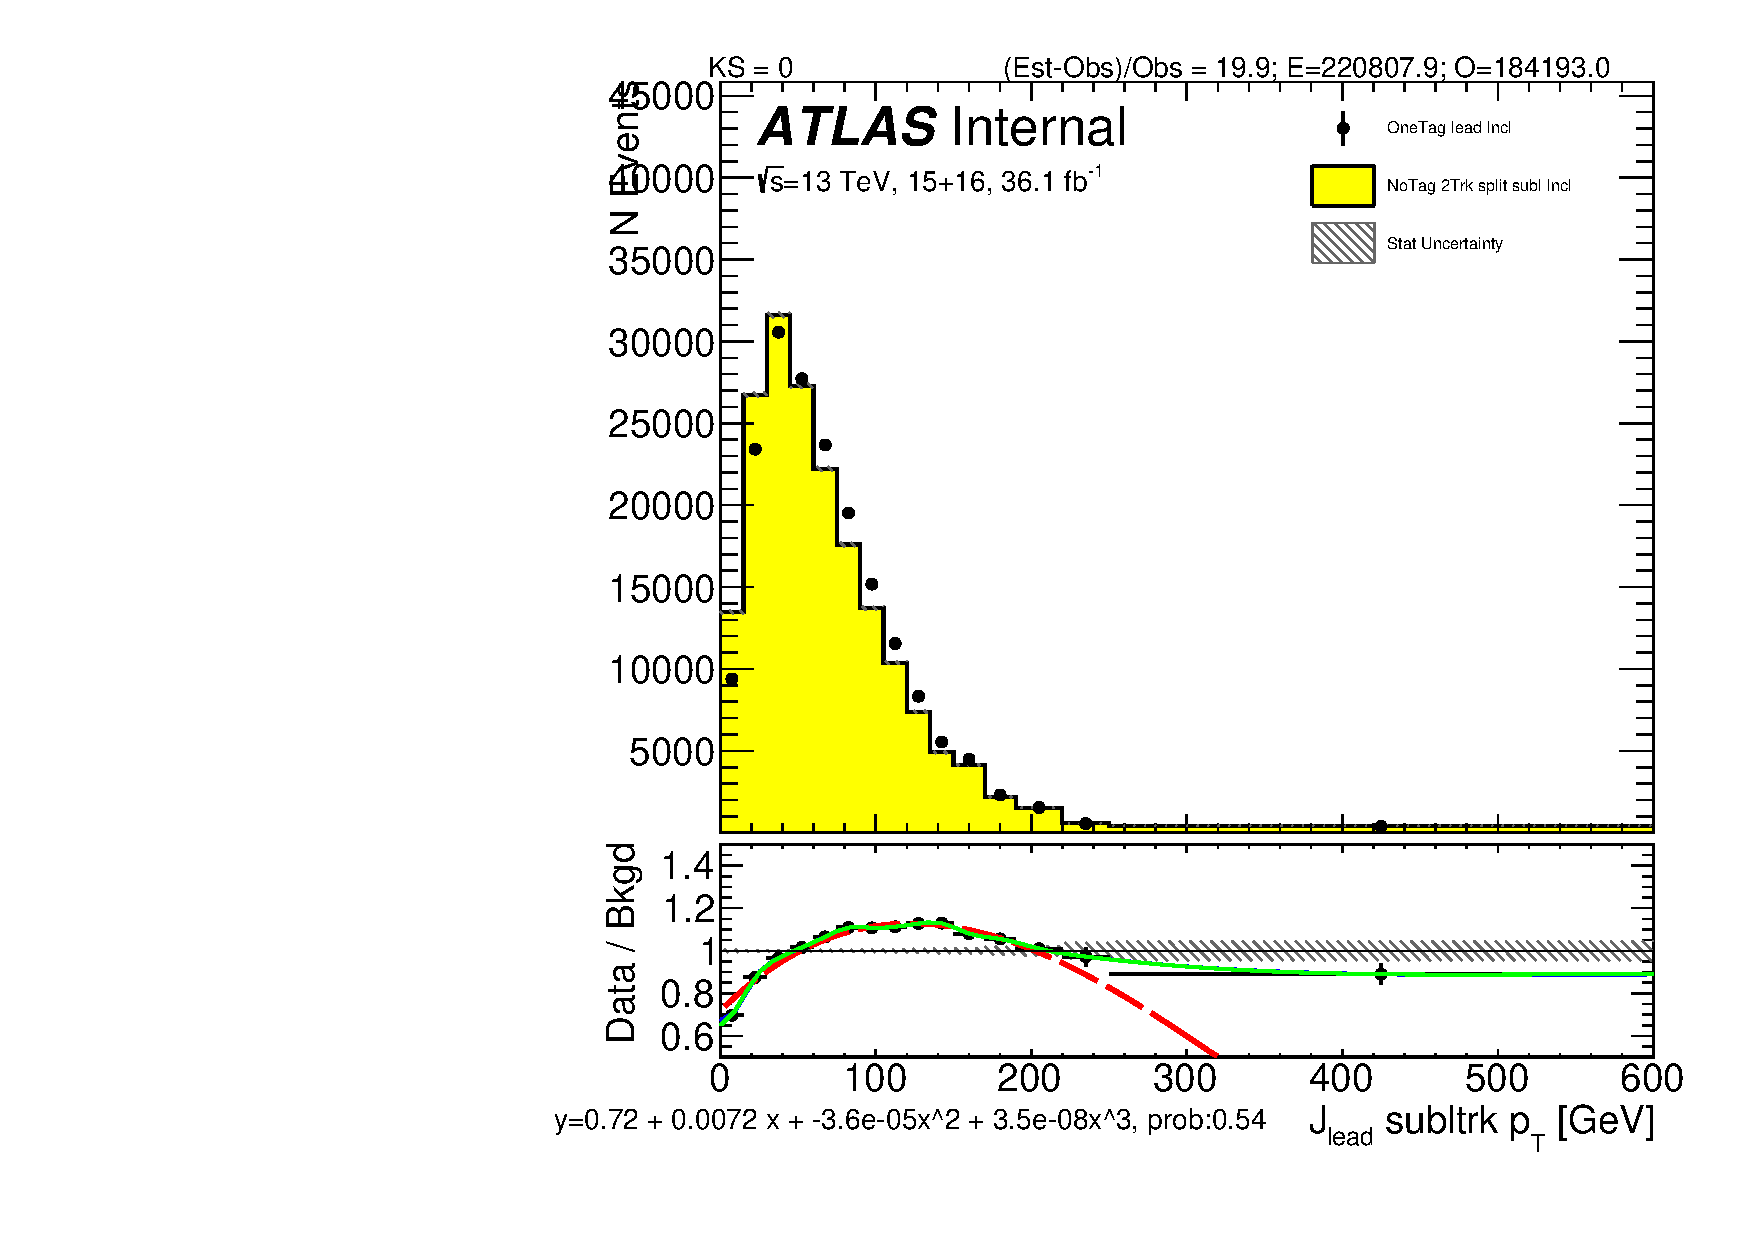
\includegraphics[width=0.32\textwidth,angle=-90]{figures/boosted/Reweight/Fits/Moriond_NoTag_2Trk_split_subl_Incl_leadHCand_trk1_Pt.pdf} \\
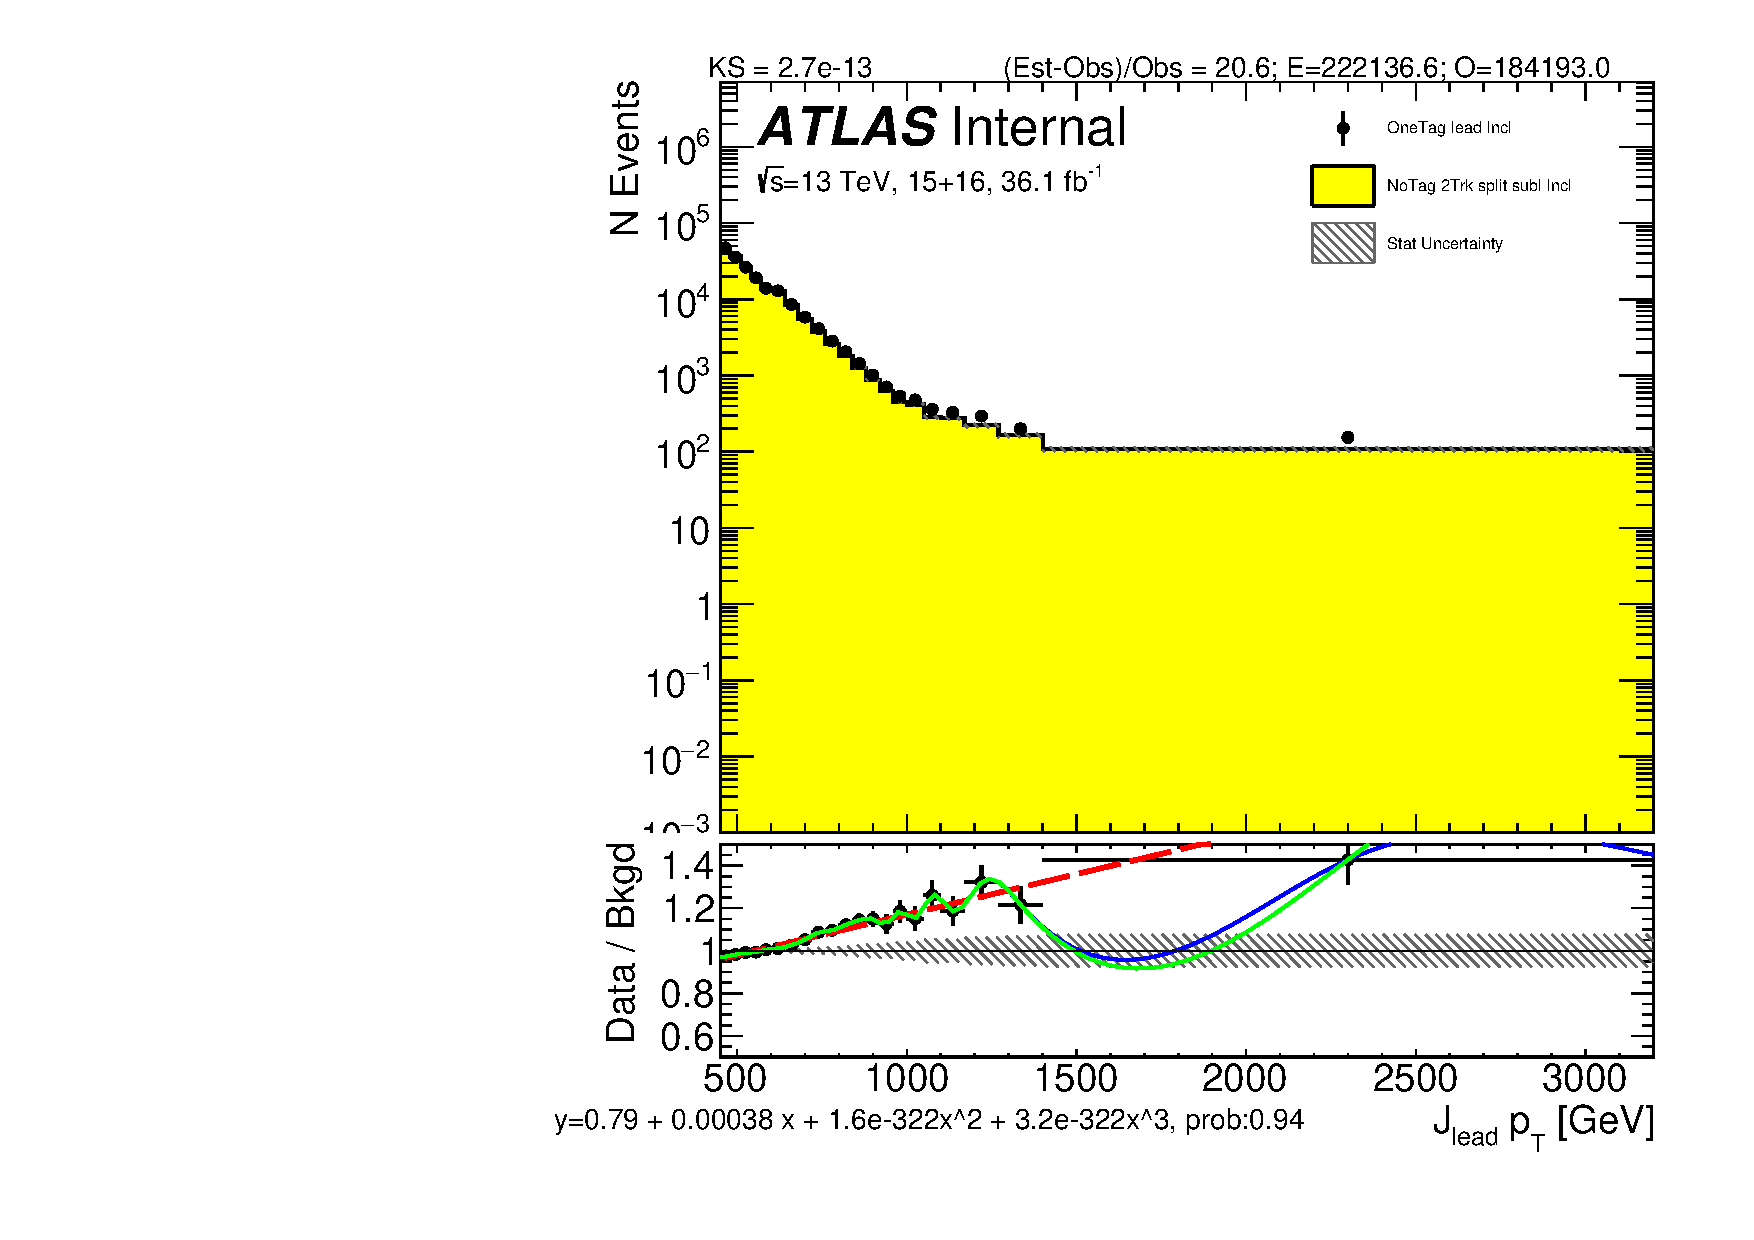
\includegraphics[width=0.32\textwidth,angle=-90]{figures/boosted/Reweight/Fits/Moriond_bkg_0_NoTag_2Trk_split_subl_Incl_leadHCand_Pt_m_1.pdf}
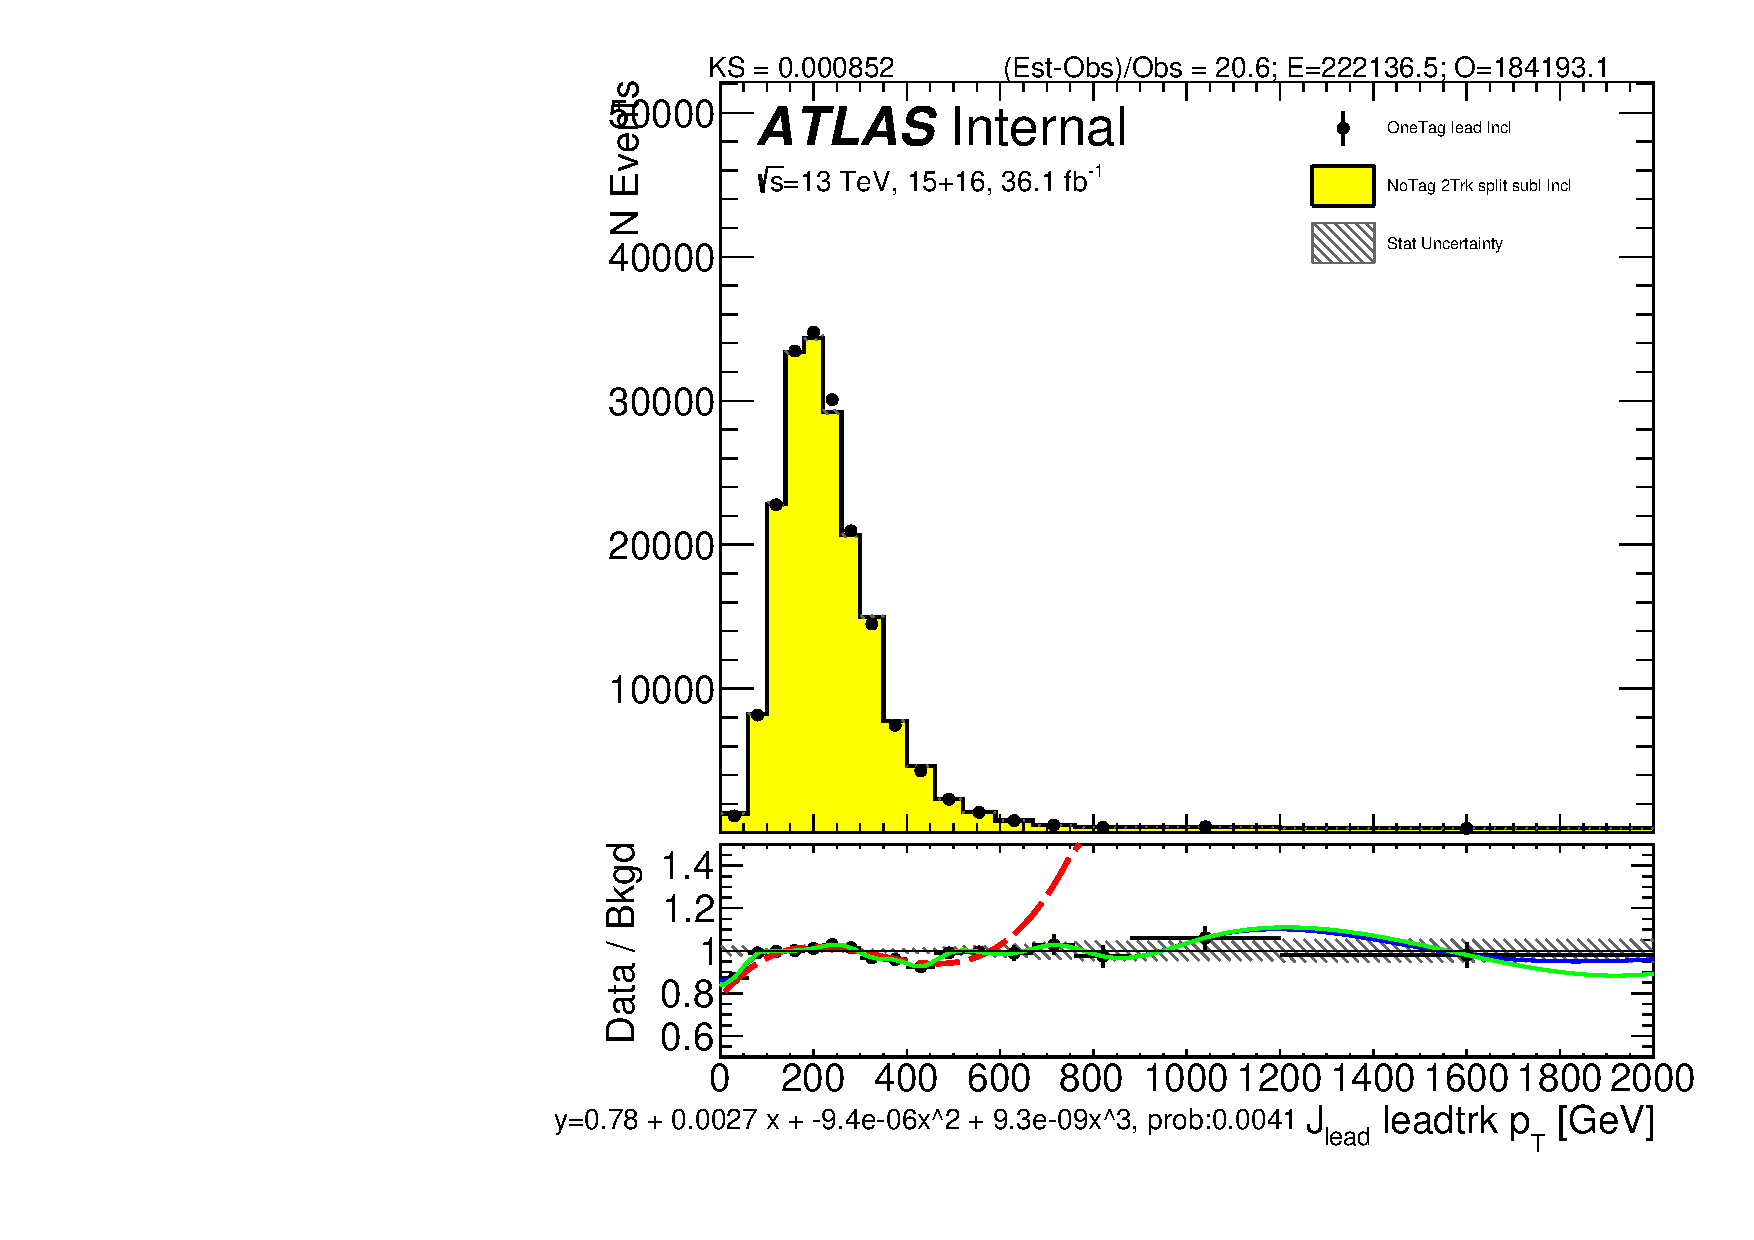
\includegraphics[width=0.32\textwidth,angle=-90]{figures/boosted/Reweight/Fits/Moriond_bkg_0_NoTag_2Trk_split_subl_Incl_leadHCand_trk0_Pt.pdf}
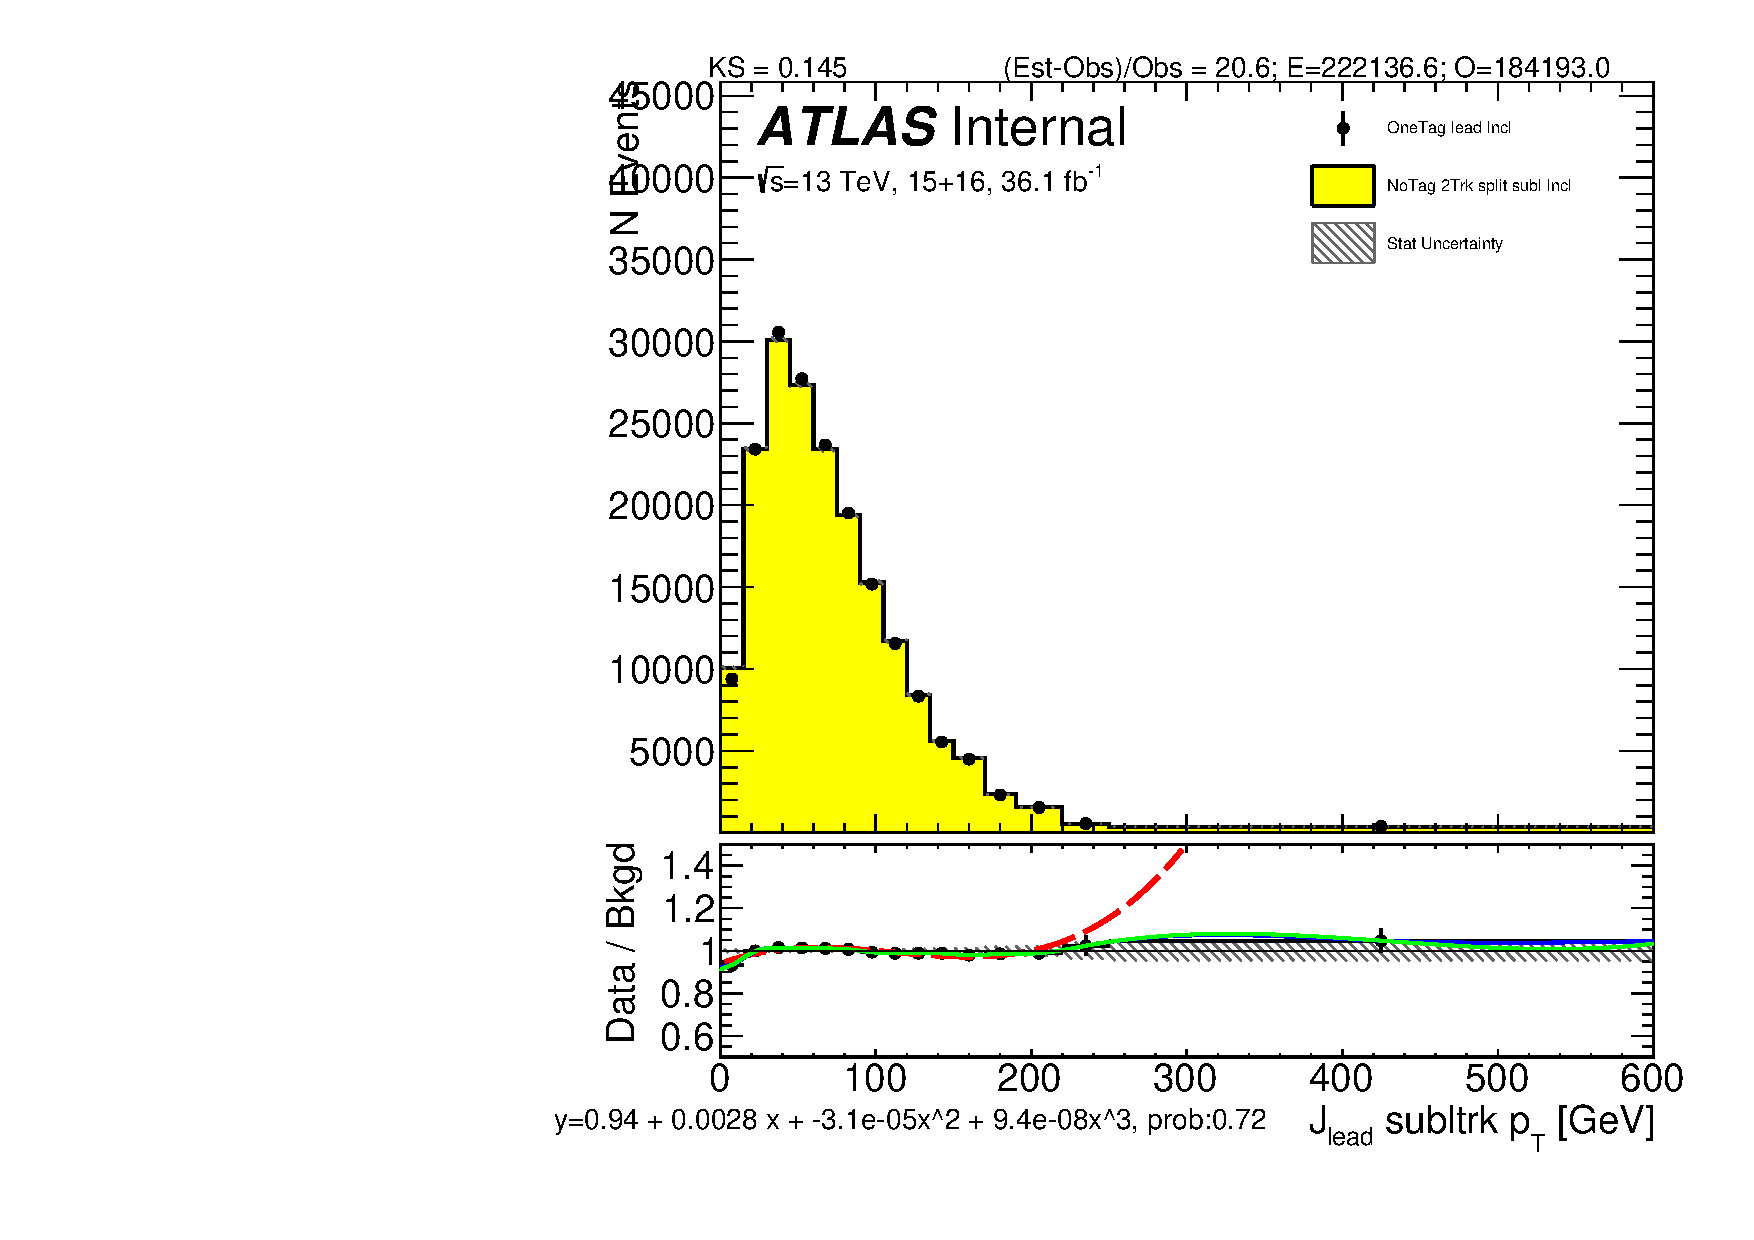
\includegraphics[width=0.32\textwidth,angle=-90]{figures/boosted/Reweight/Fits/Moriond_bkg_0_NoTag_2Trk_split_subl_Incl_leadHCand_trk1_Pt.pdf} \\
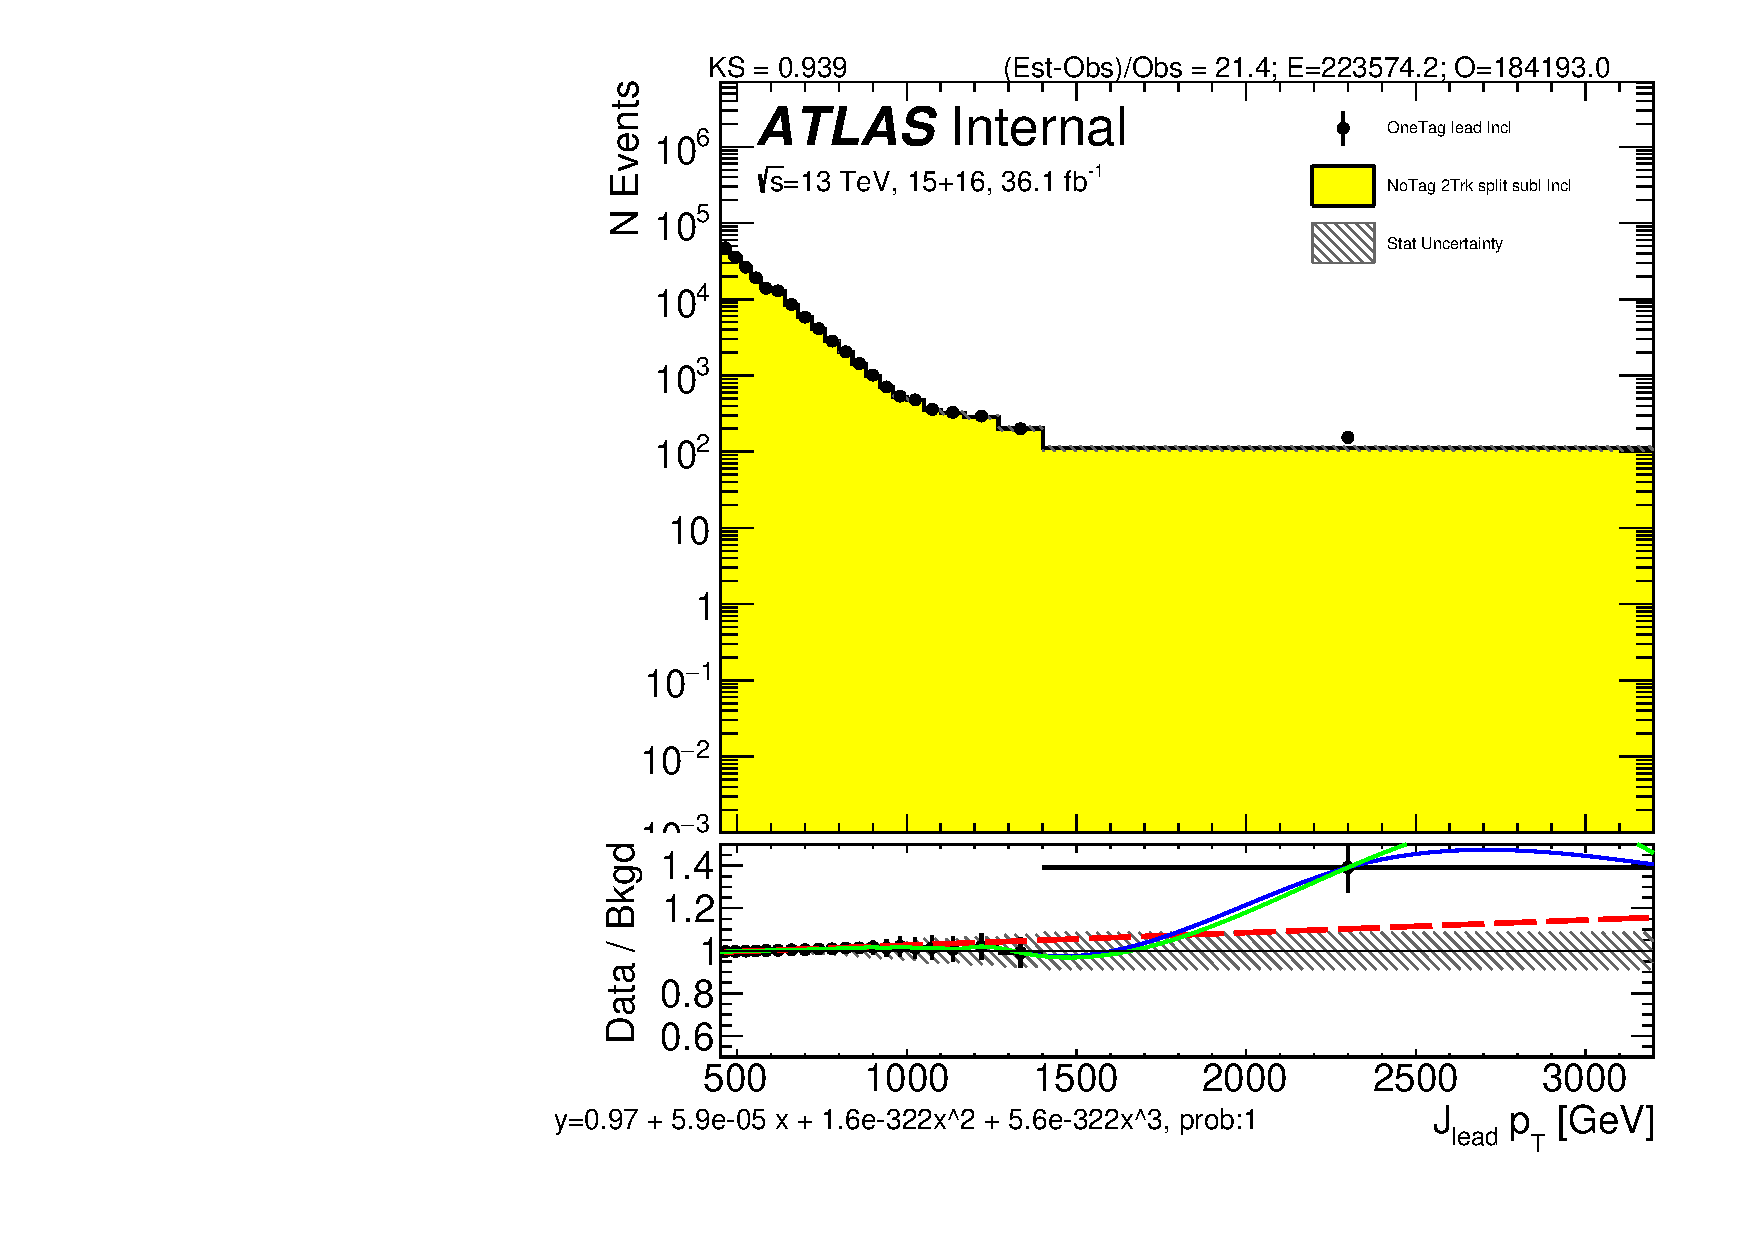
\includegraphics[width=0.32\textwidth,angle=-90]{figures/boosted/Reweight/Fits/Moriond_bkg_3_NoTag_2Trk_split_subl_Incl_leadHCand_Pt_m_1.pdf}
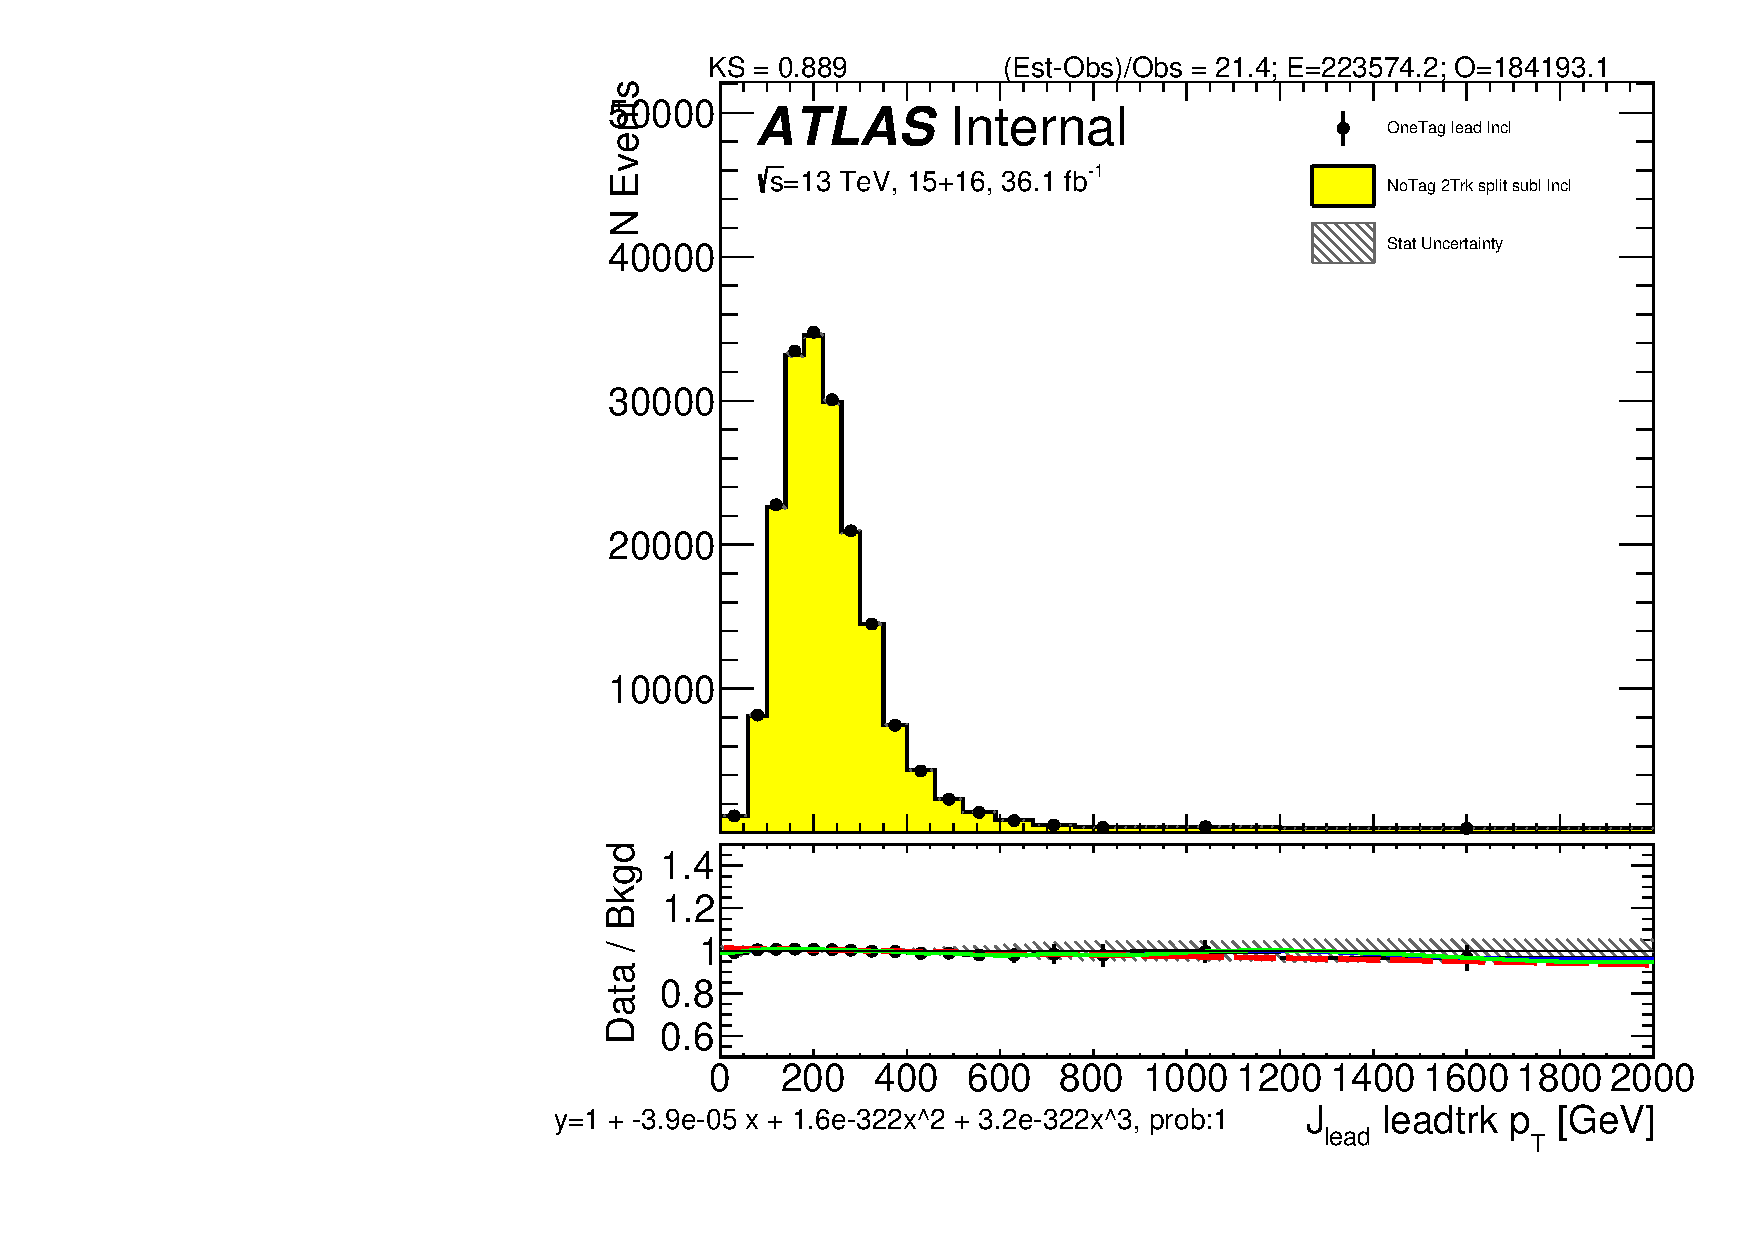
\includegraphics[width=0.32\textwidth,angle=-90]{figures/boosted/Reweight/Fits/Moriond_bkg_3_NoTag_2Trk_split_subl_Incl_leadHCand_trk0_Pt.pdf}
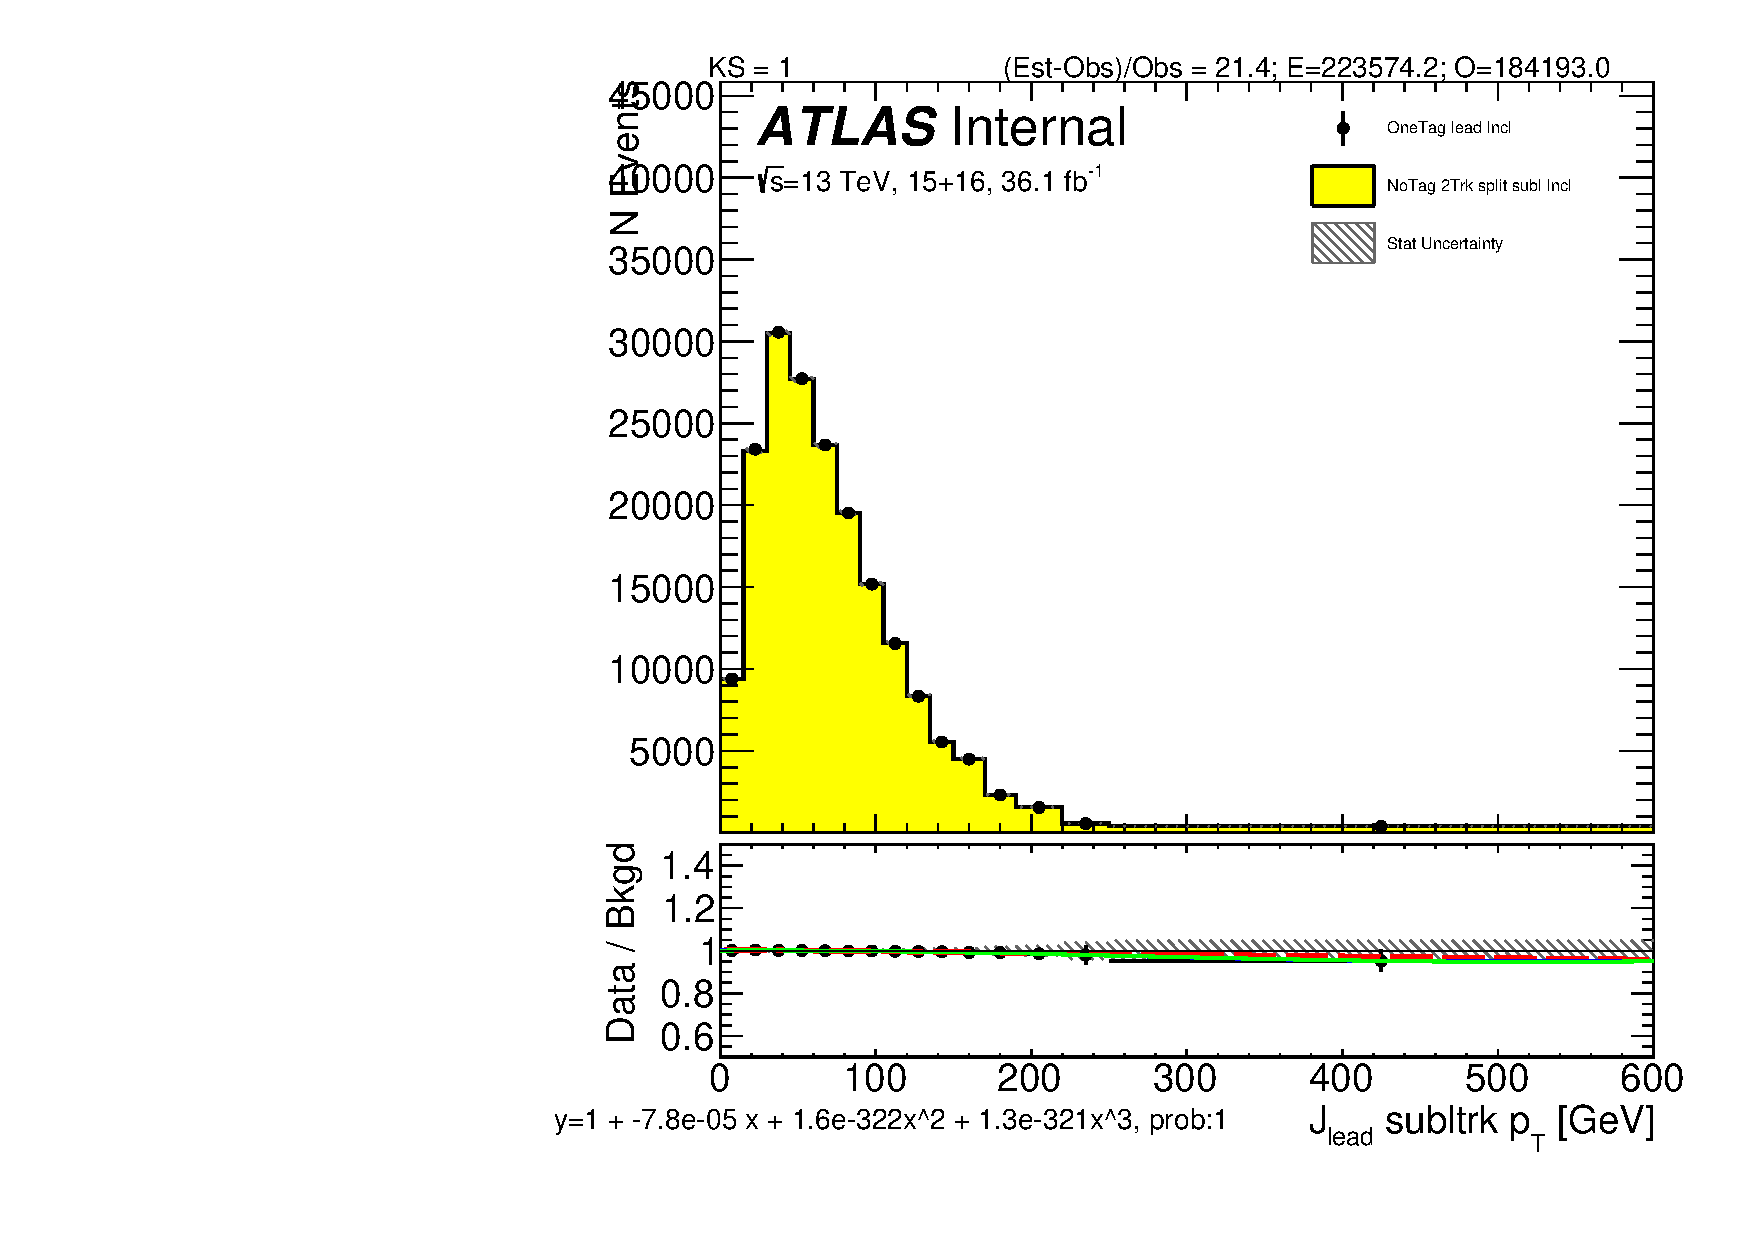
\includegraphics[width=0.32\textwidth,angle=-90]{figures/boosted/Reweight/Fits/Moriond_bkg_3_NoTag_2Trk_split_subl_Incl_leadHCand_trk1_Pt.pdf} \\
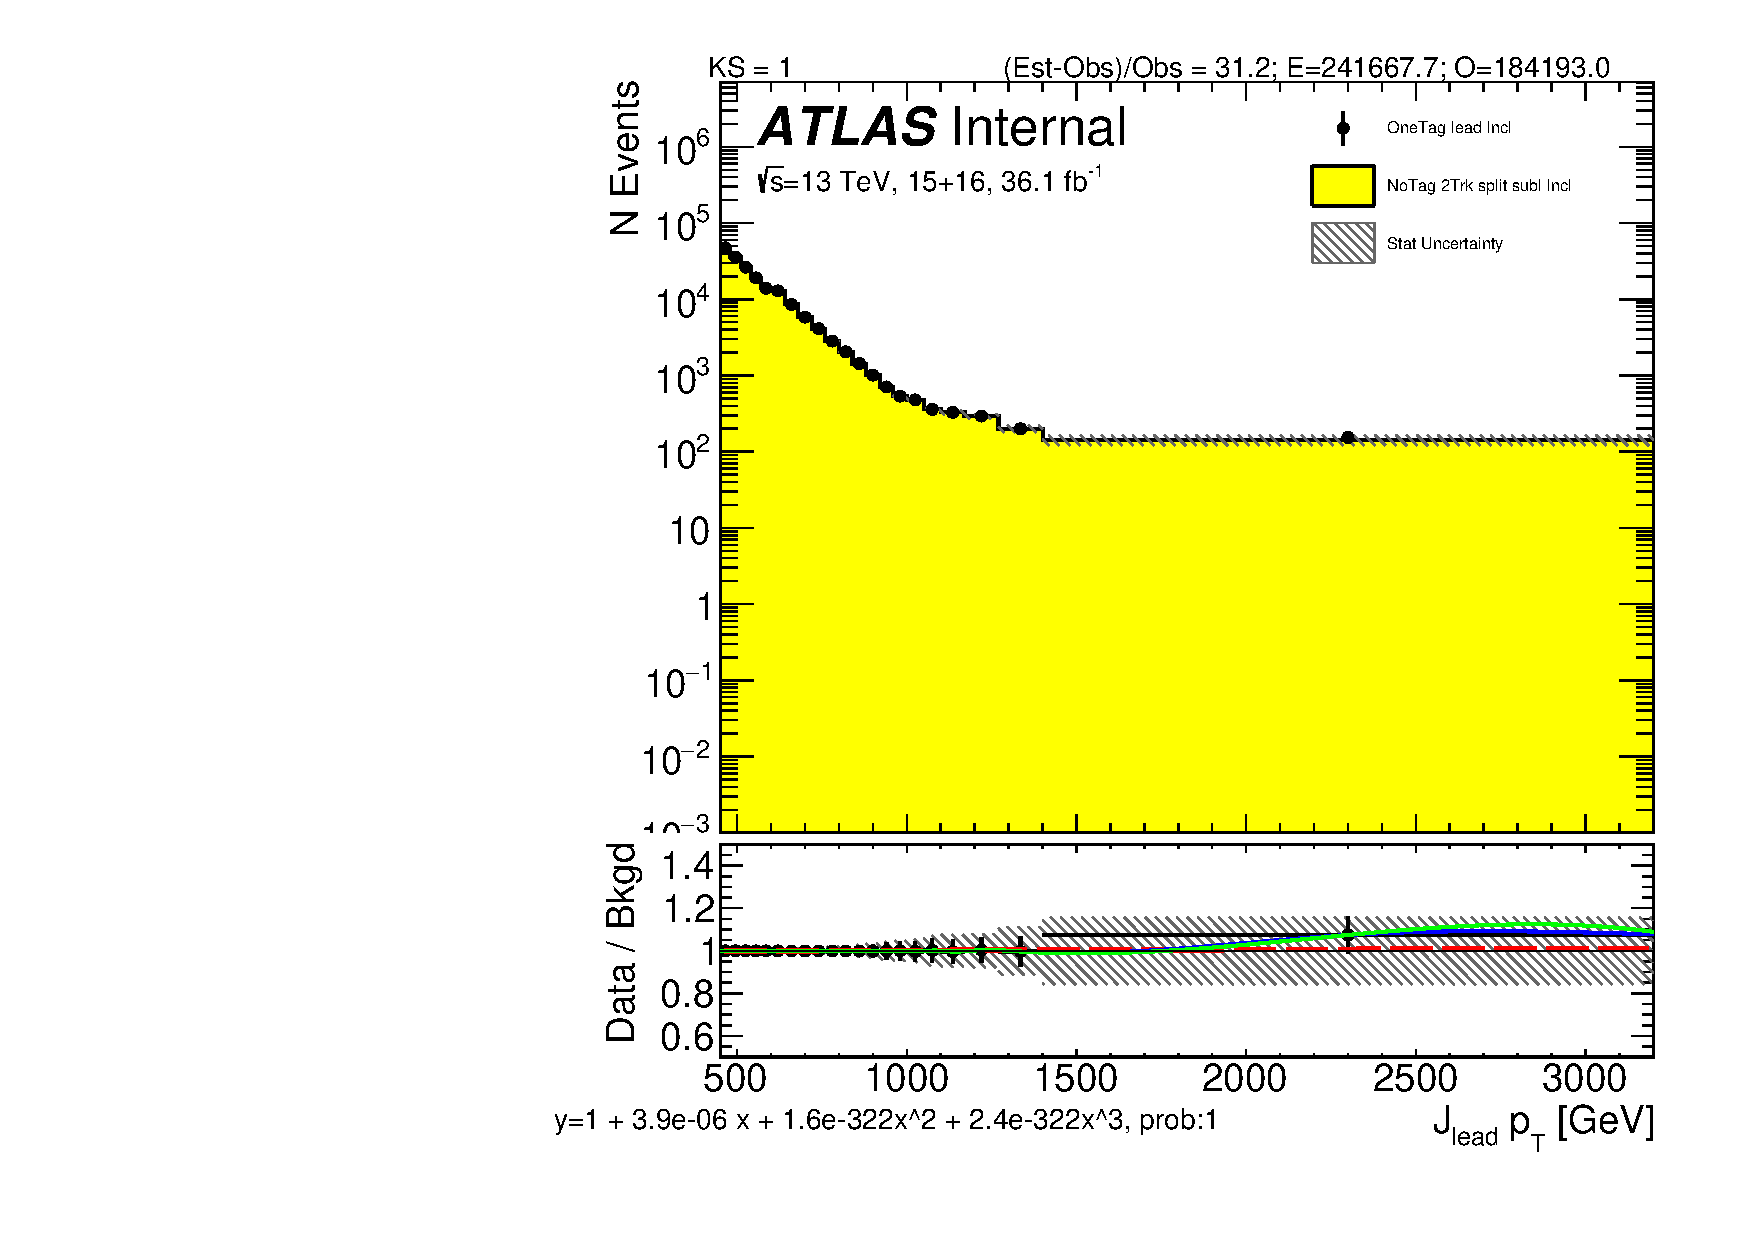
\includegraphics[width=0.32\textwidth,angle=-90]{figures/boosted/Reweight/Fits/Moriond_bkg_9_NoTag_2Trk_split_subl_Incl_leadHCand_Pt_m_1.pdf}
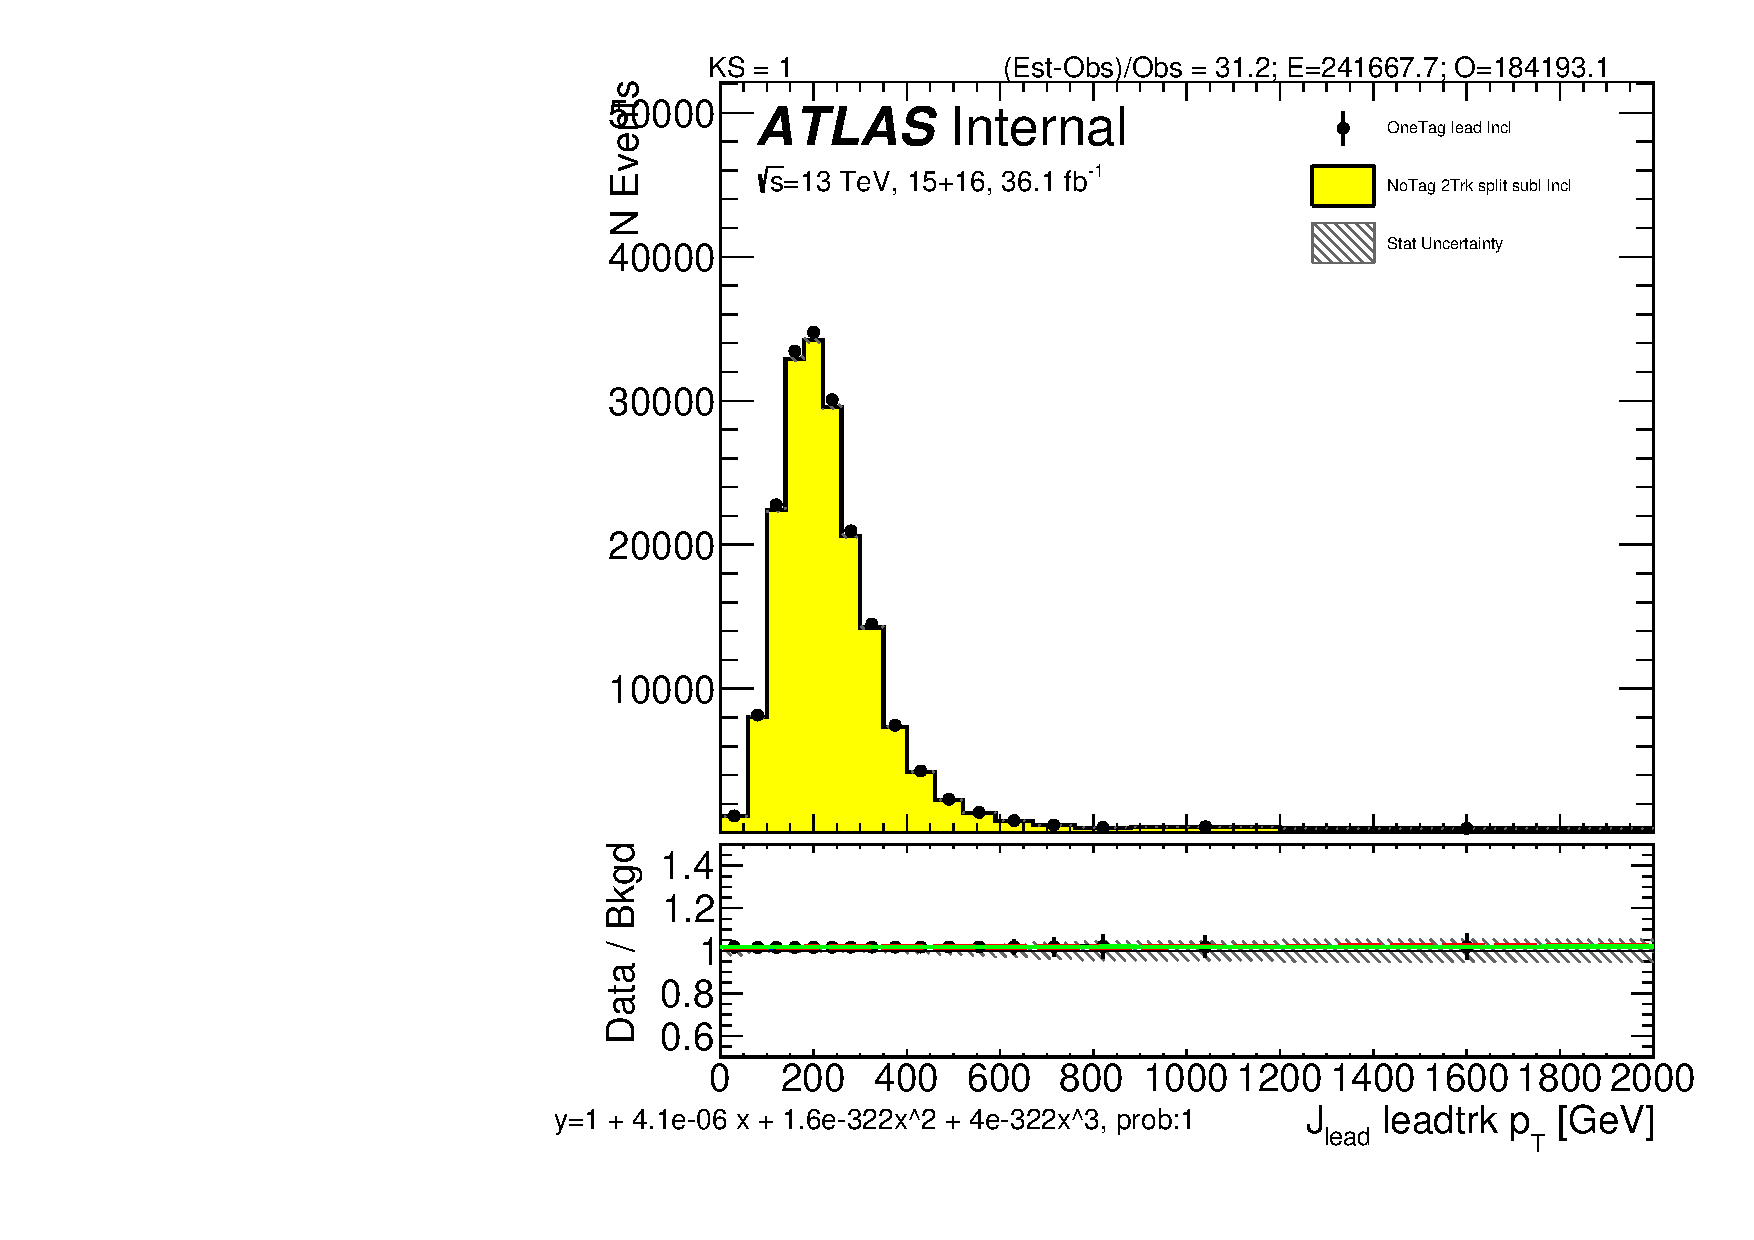
\includegraphics[width=0.32\textwidth,angle=-90]{figures/boosted/Reweight/Fits/Moriond_bkg_9_NoTag_2Trk_split_subl_Incl_leadHCand_trk0_Pt.pdf}
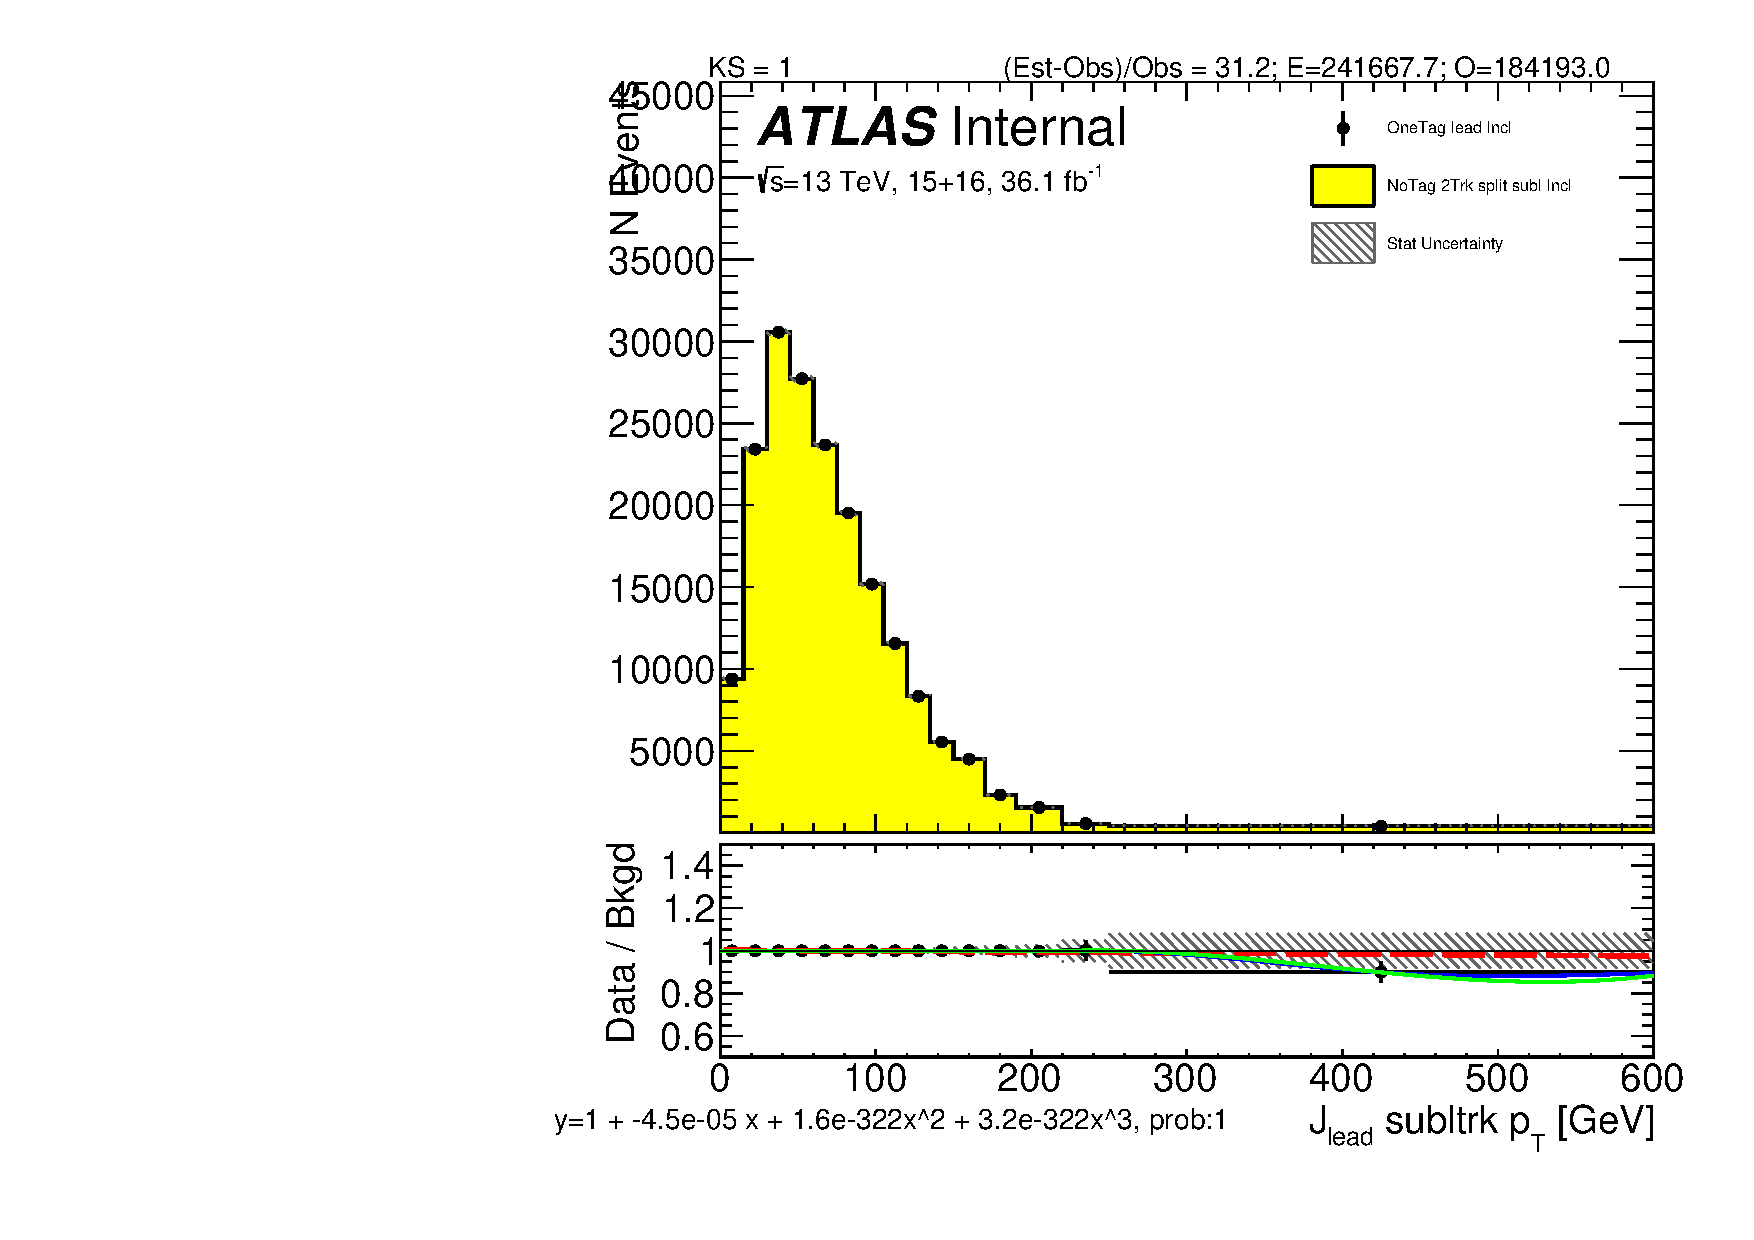
\includegraphics[width=0.32\textwidth,angle=-90]{figures/boosted/Reweight/Fits/Moriond_bkg_9_NoTag_2Trk_split_subl_Incl_leadHCand_trk1_Pt.pdf} \\
\caption{For $2bs$ background estimate: the fits to the ratio of the data in the $1b$ category, of the leading Higgs candidate $1b$-tagged events's leading Higgs candidate distributions(black point), over the sublleading Higgs candidate $1b$-tagged events's leading Higgs candidate distributions(yellow). Distributions and fits to the estimated QCD background for large-$R$ jet $p_{T}$ (left),  the large-$R$ jet's leading trackjet $p_T$ (middle), and large-$R$ jet's subleading trackjet $p_T$ (right) are shown.  Figure are shown before reweighting (top row), after the first iteration(second row), after the fourth iteration(third row), and after the last iteration (bottow row). The green line is the spline extrapolation; and the red line is a polynomial fit.}
\label{fig:rw-2bs-subl}
\end{center}
\end{figure*}

\begin{figure*}[htbp!]
\begin{center}
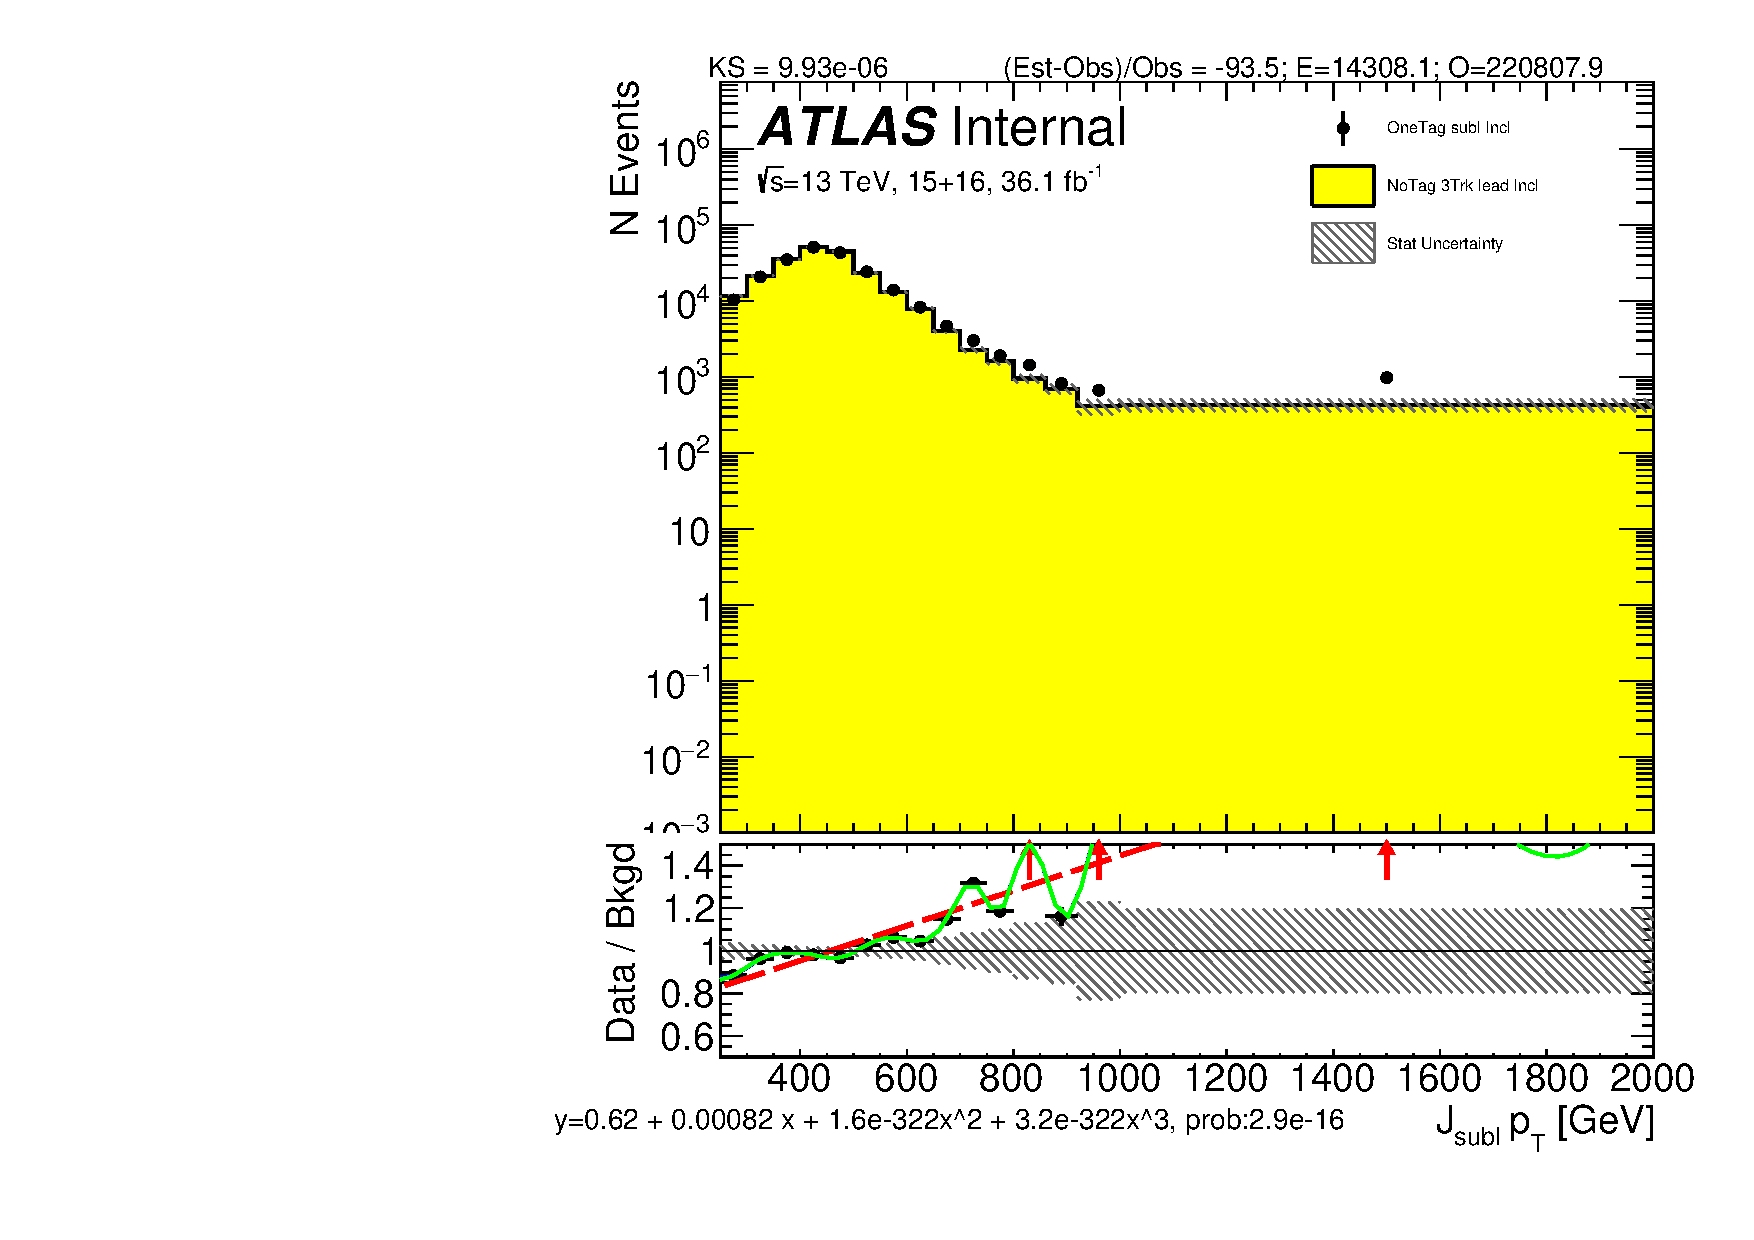
\includegraphics[width=0.32\textwidth,angle=-90]{figures/boosted/Reweight/Fits/Moriond_NoTag_3Trk_lead_Incl_sublHCand_Pt_m_1.pdf}
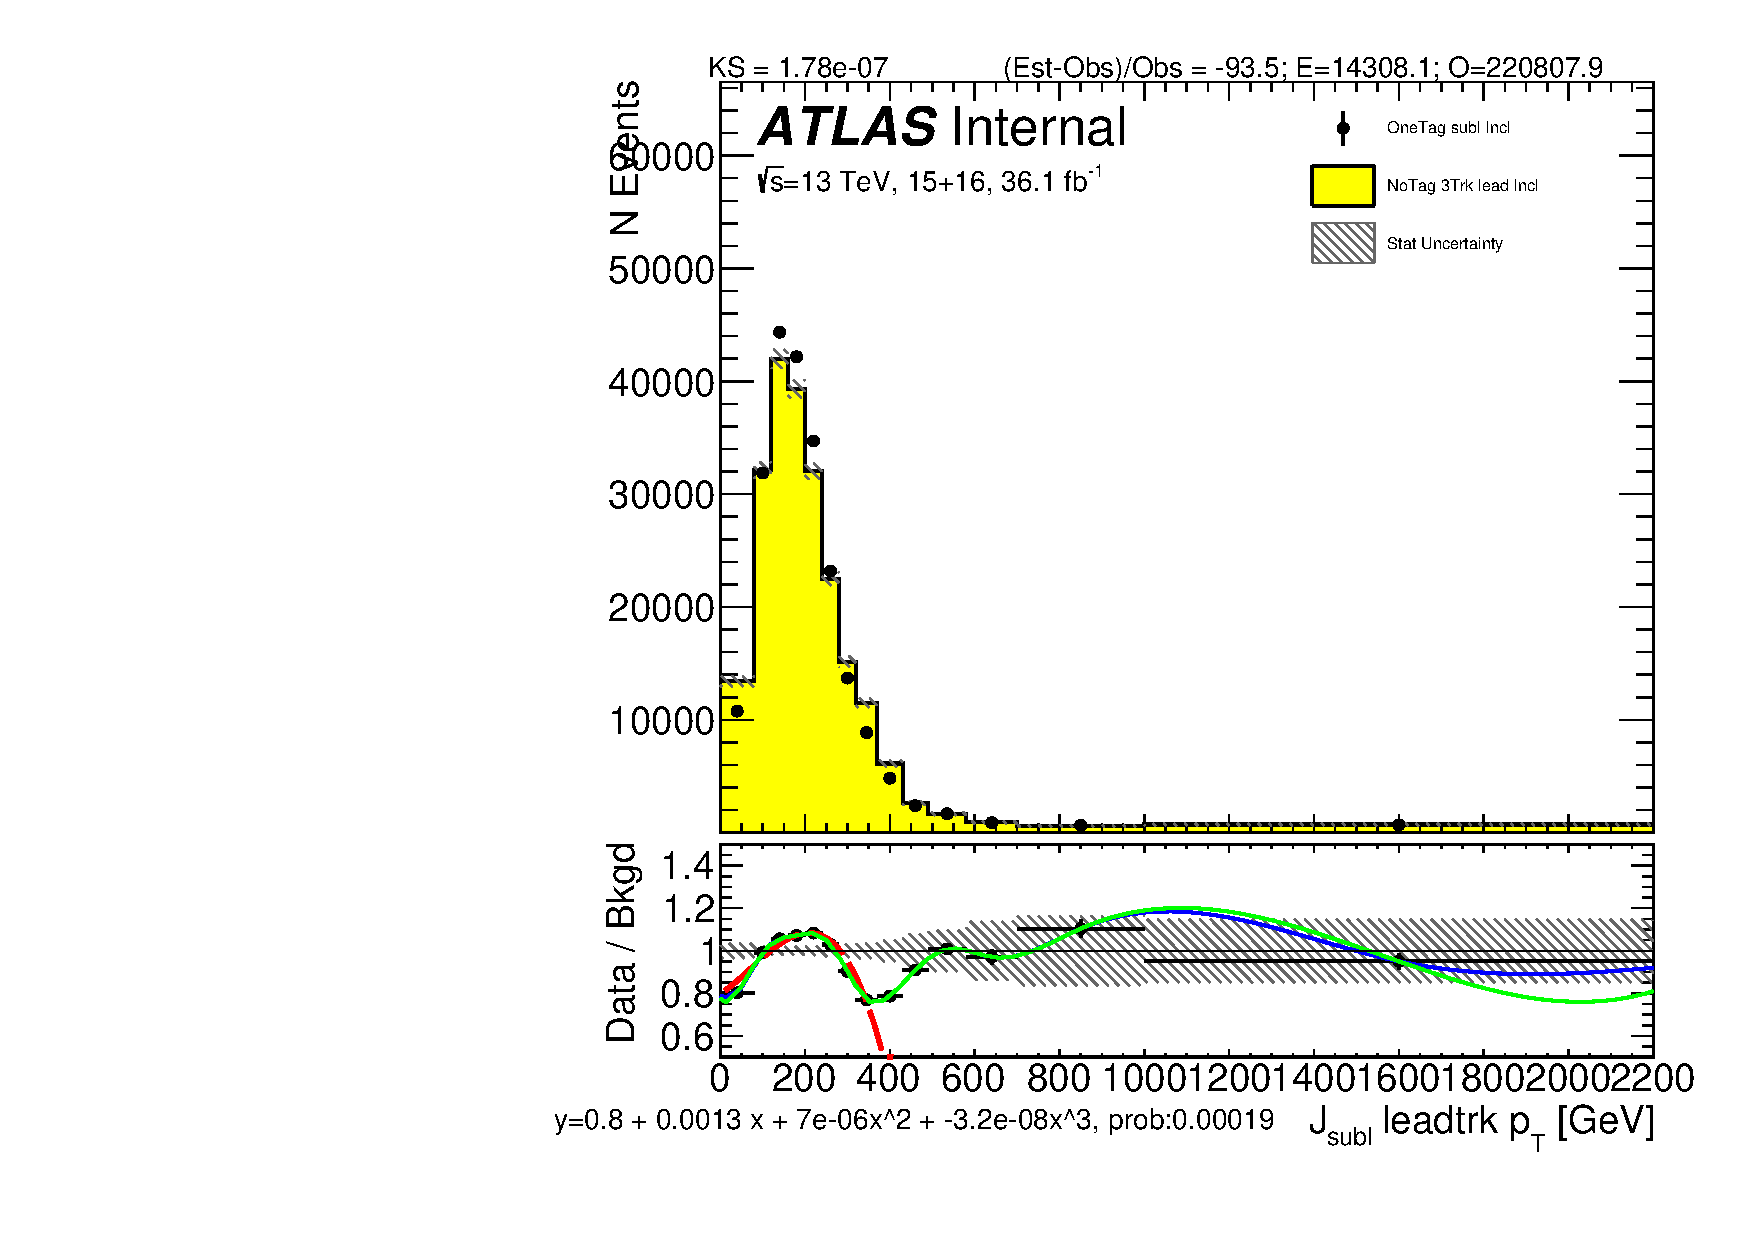
\includegraphics[width=0.32\textwidth,angle=-90]{figures/boosted/Reweight/Fits/Moriond_NoTag_3Trk_lead_Incl_sublHCand_trk0_Pt.pdf}
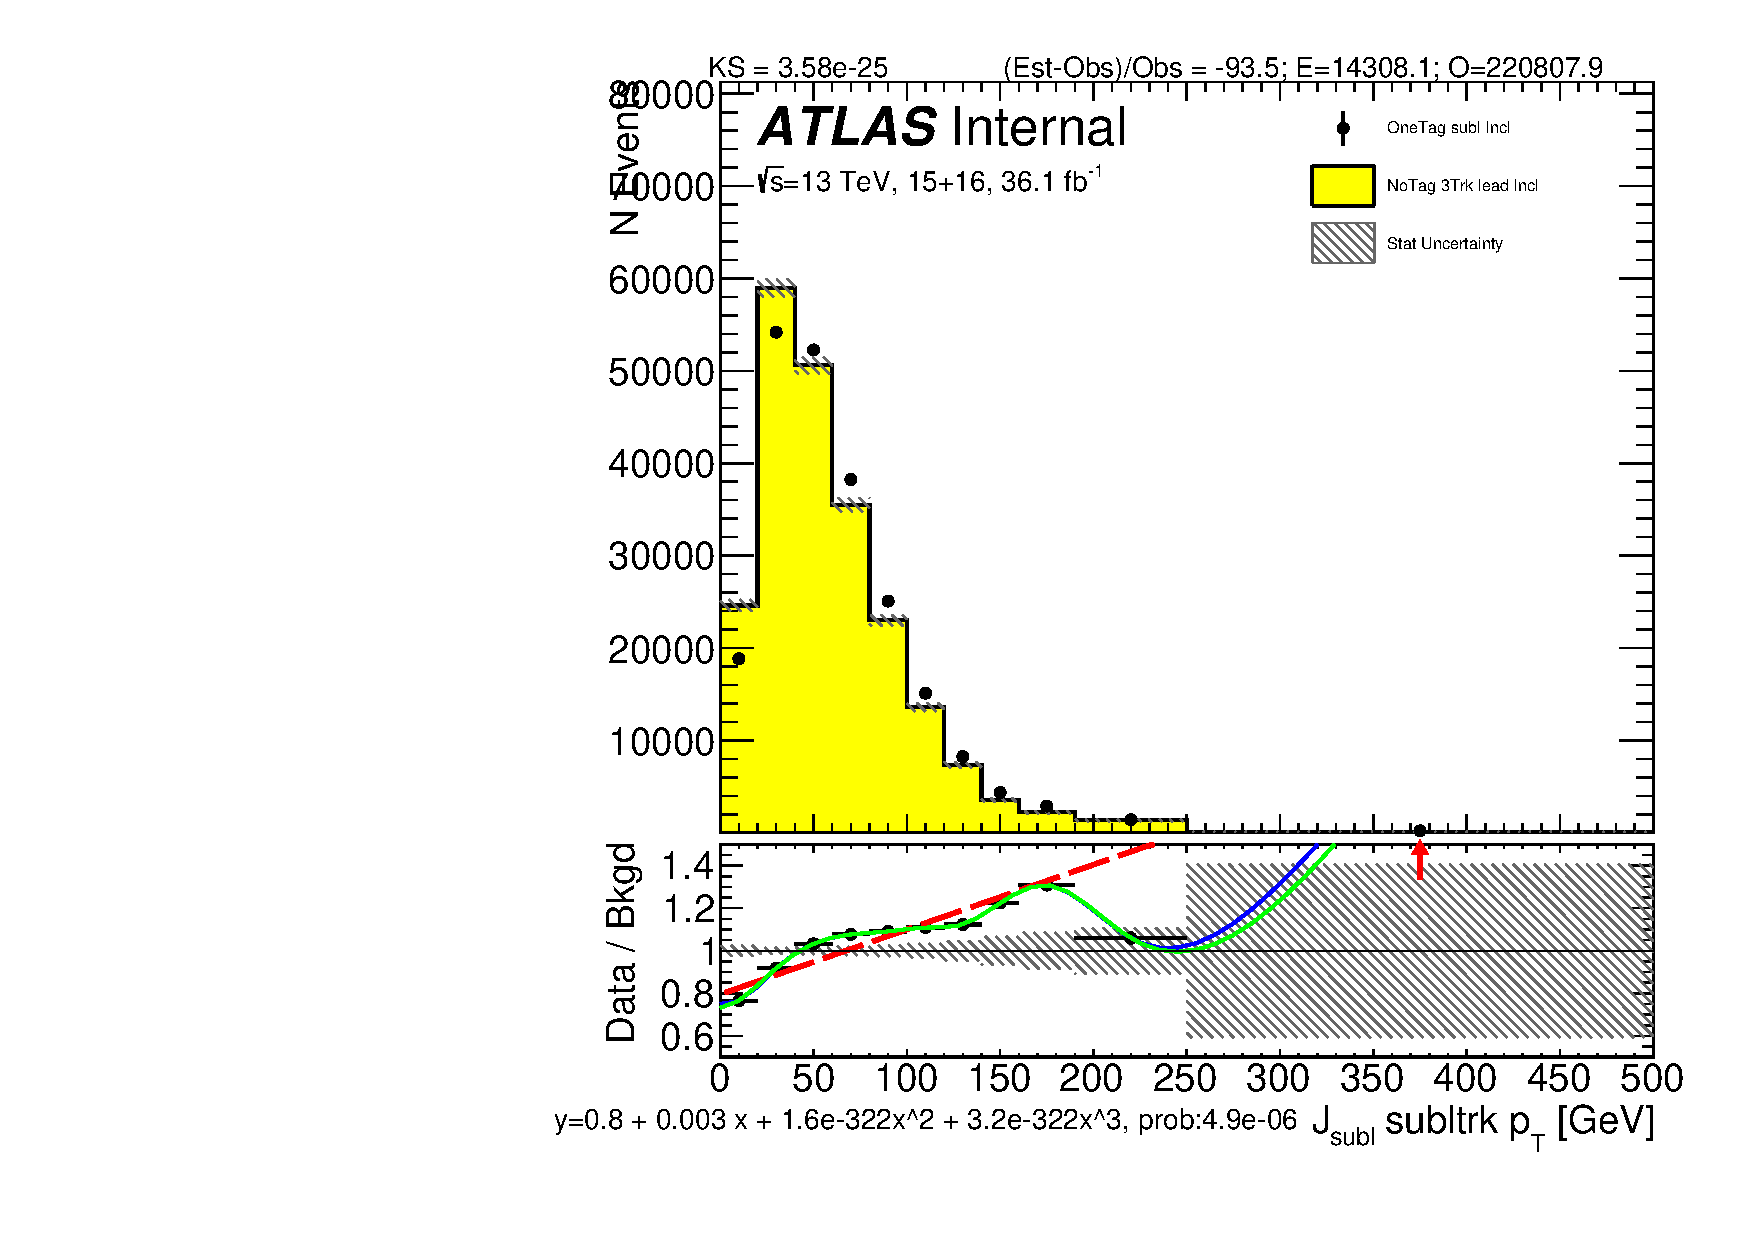
\includegraphics[width=0.32\textwidth,angle=-90]{figures/boosted/Reweight/Fits/Moriond_NoTag_3Trk_lead_Incl_sublHCand_trk1_Pt.pdf} \\
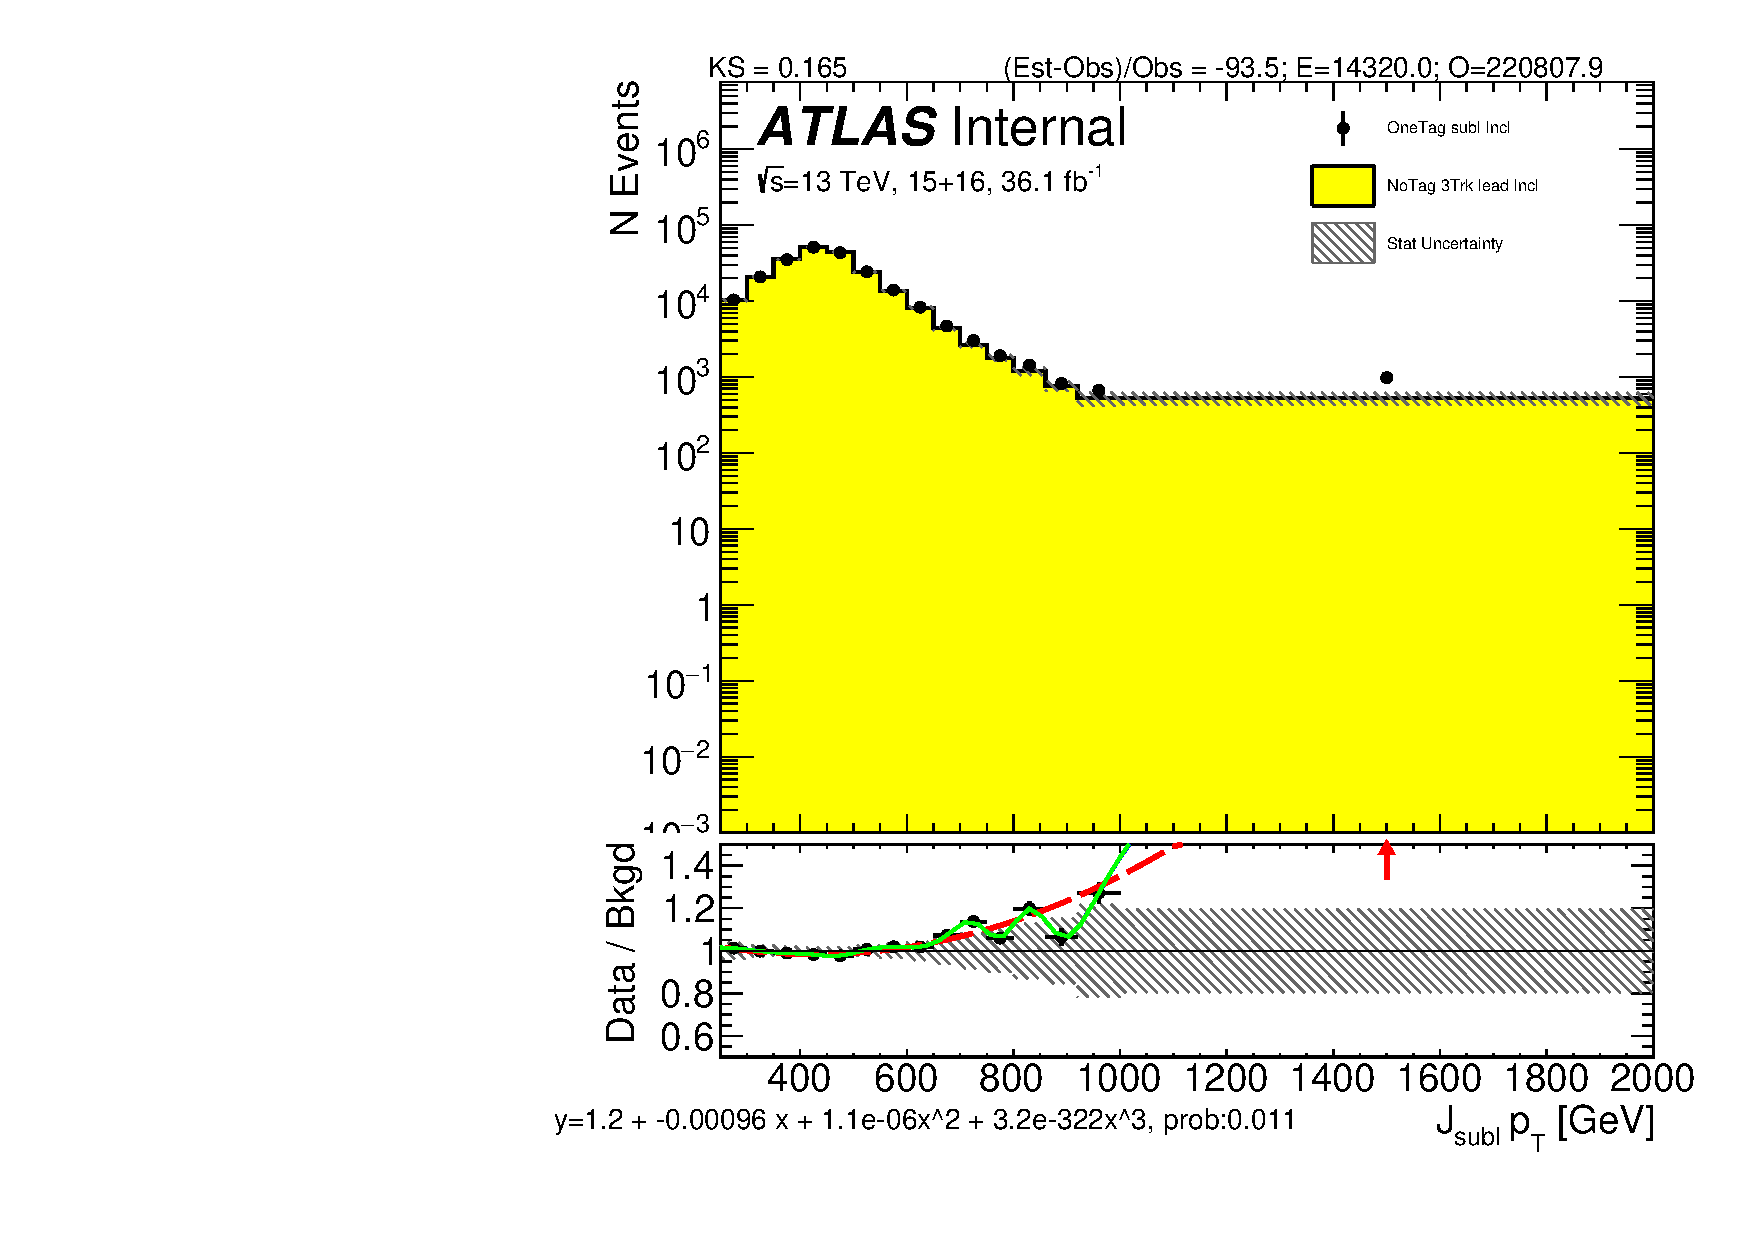
\includegraphics[width=0.32\textwidth,angle=-90]{figures/boosted/Reweight/Fits/Moriond_bkg_0_NoTag_3Trk_lead_Incl_sublHCand_Pt_m_1.pdf}
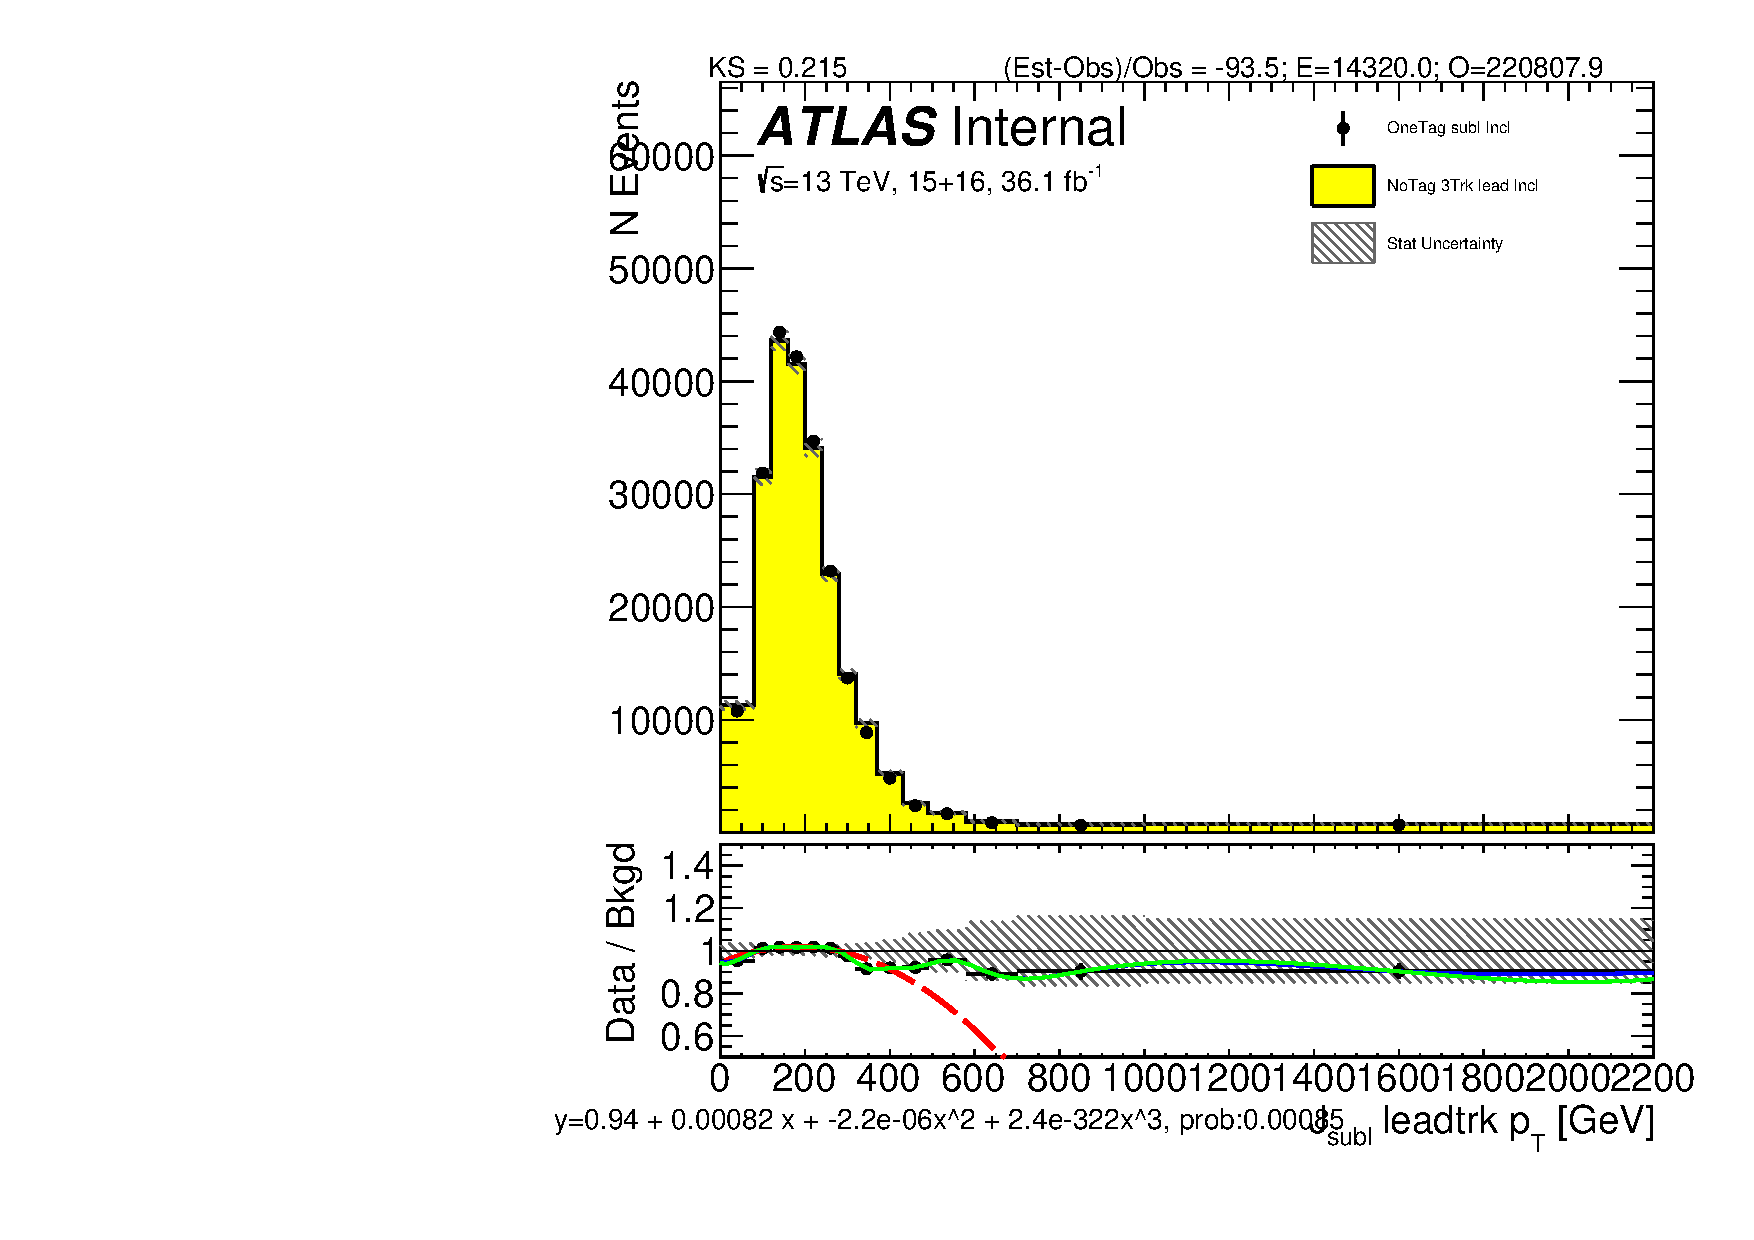
\includegraphics[width=0.32\textwidth,angle=-90]{figures/boosted/Reweight/Fits/Moriond_bkg_0_NoTag_3Trk_lead_Incl_sublHCand_trk0_Pt.pdf}
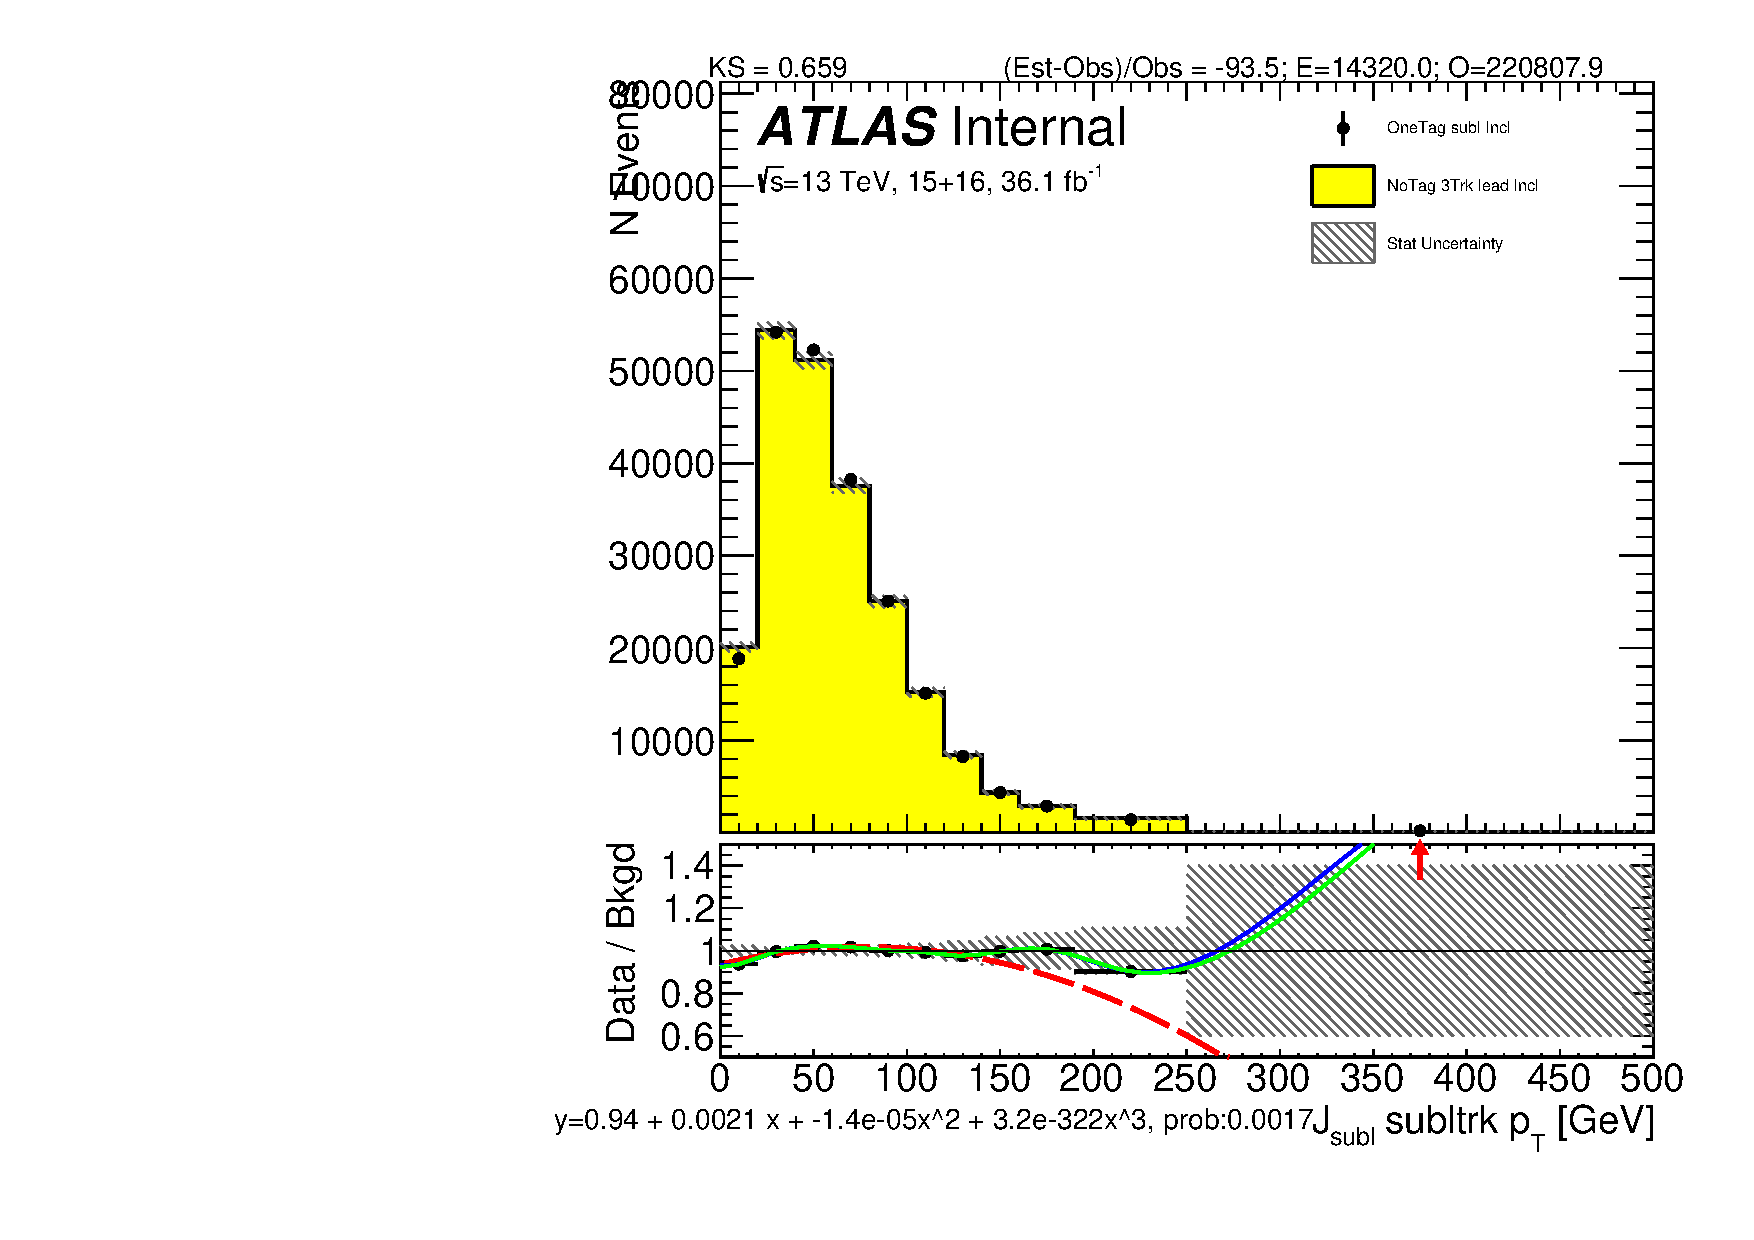
\includegraphics[width=0.32\textwidth,angle=-90]{figures/boosted/Reweight/Fits/Moriond_bkg_0_NoTag_3Trk_lead_Incl_sublHCand_trk1_Pt.pdf} \\
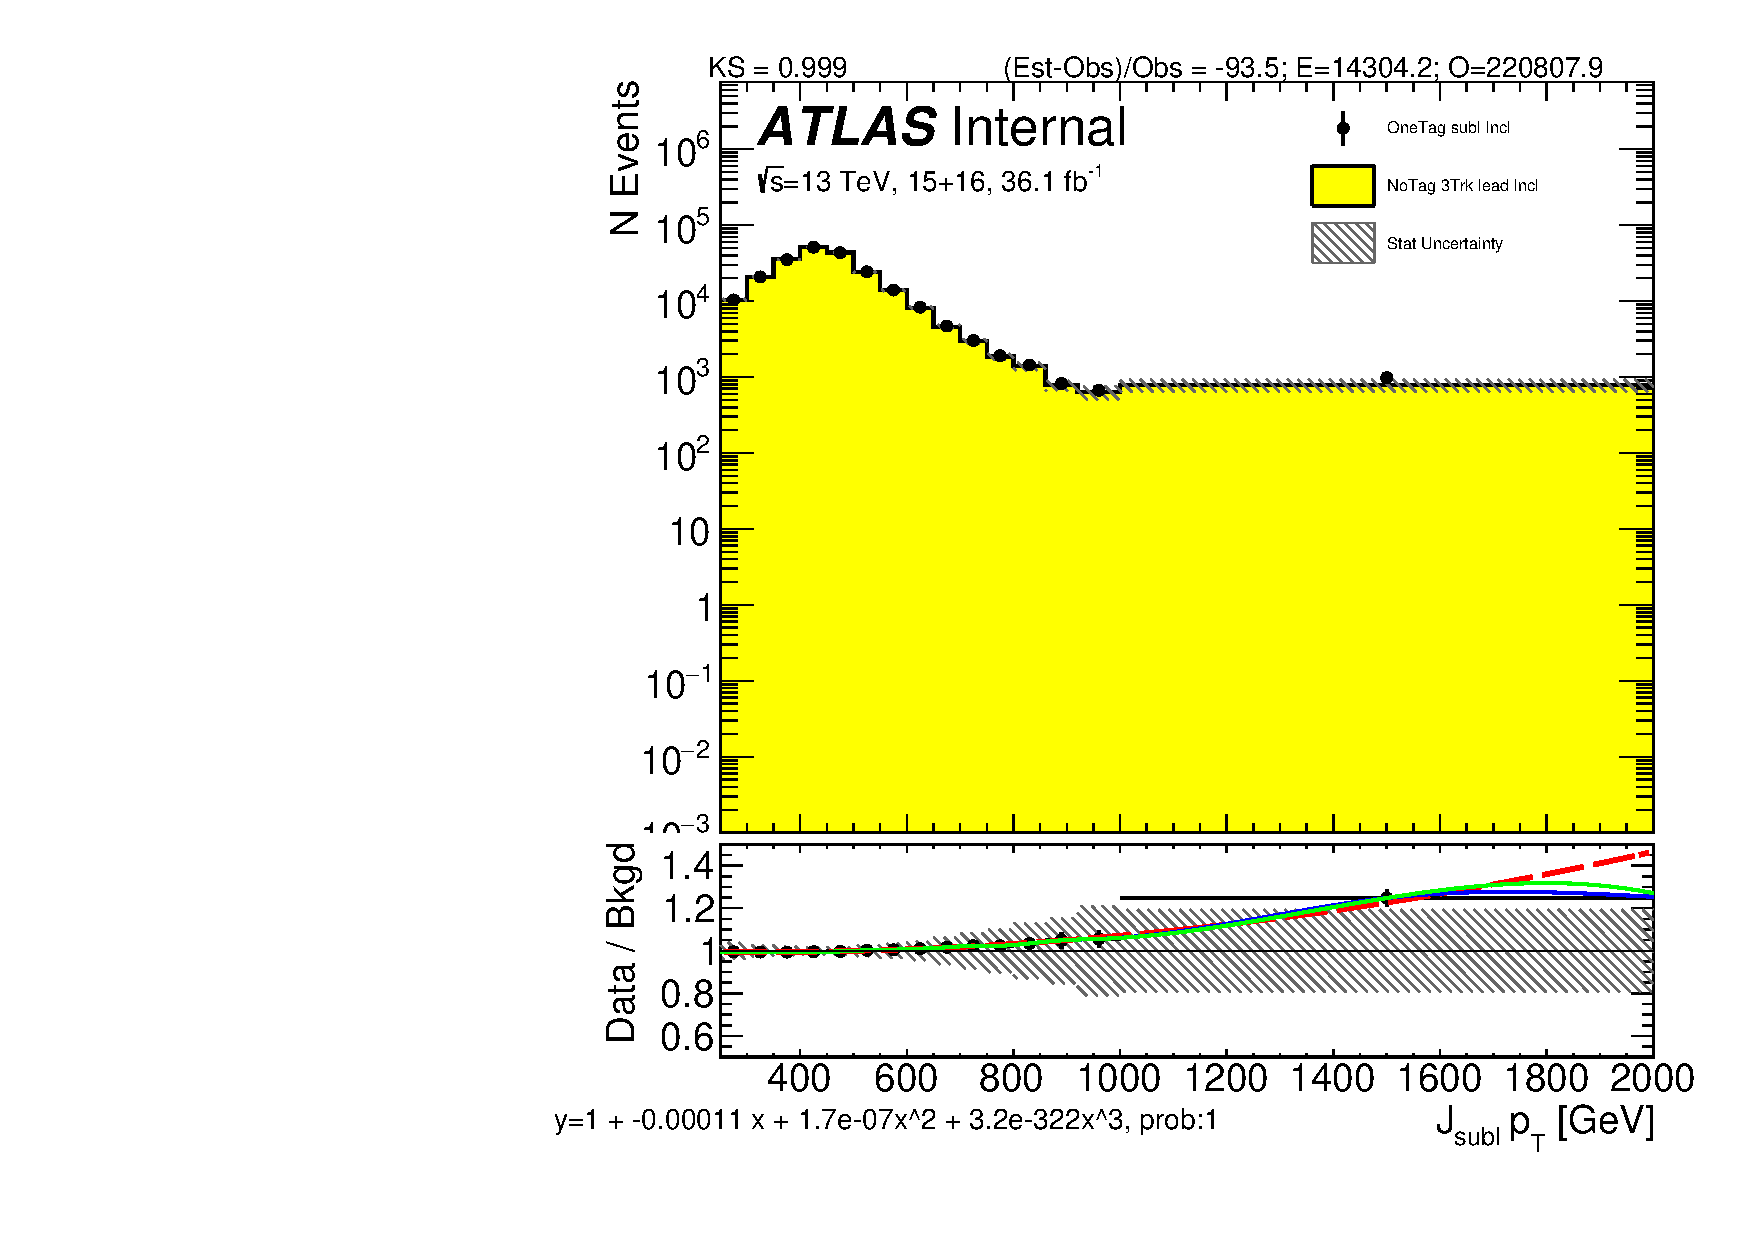
\includegraphics[width=0.32\textwidth,angle=-90]{figures/boosted/Reweight/Fits/Moriond_bkg_3_NoTag_3Trk_lead_Incl_sublHCand_Pt_m_1.pdf}
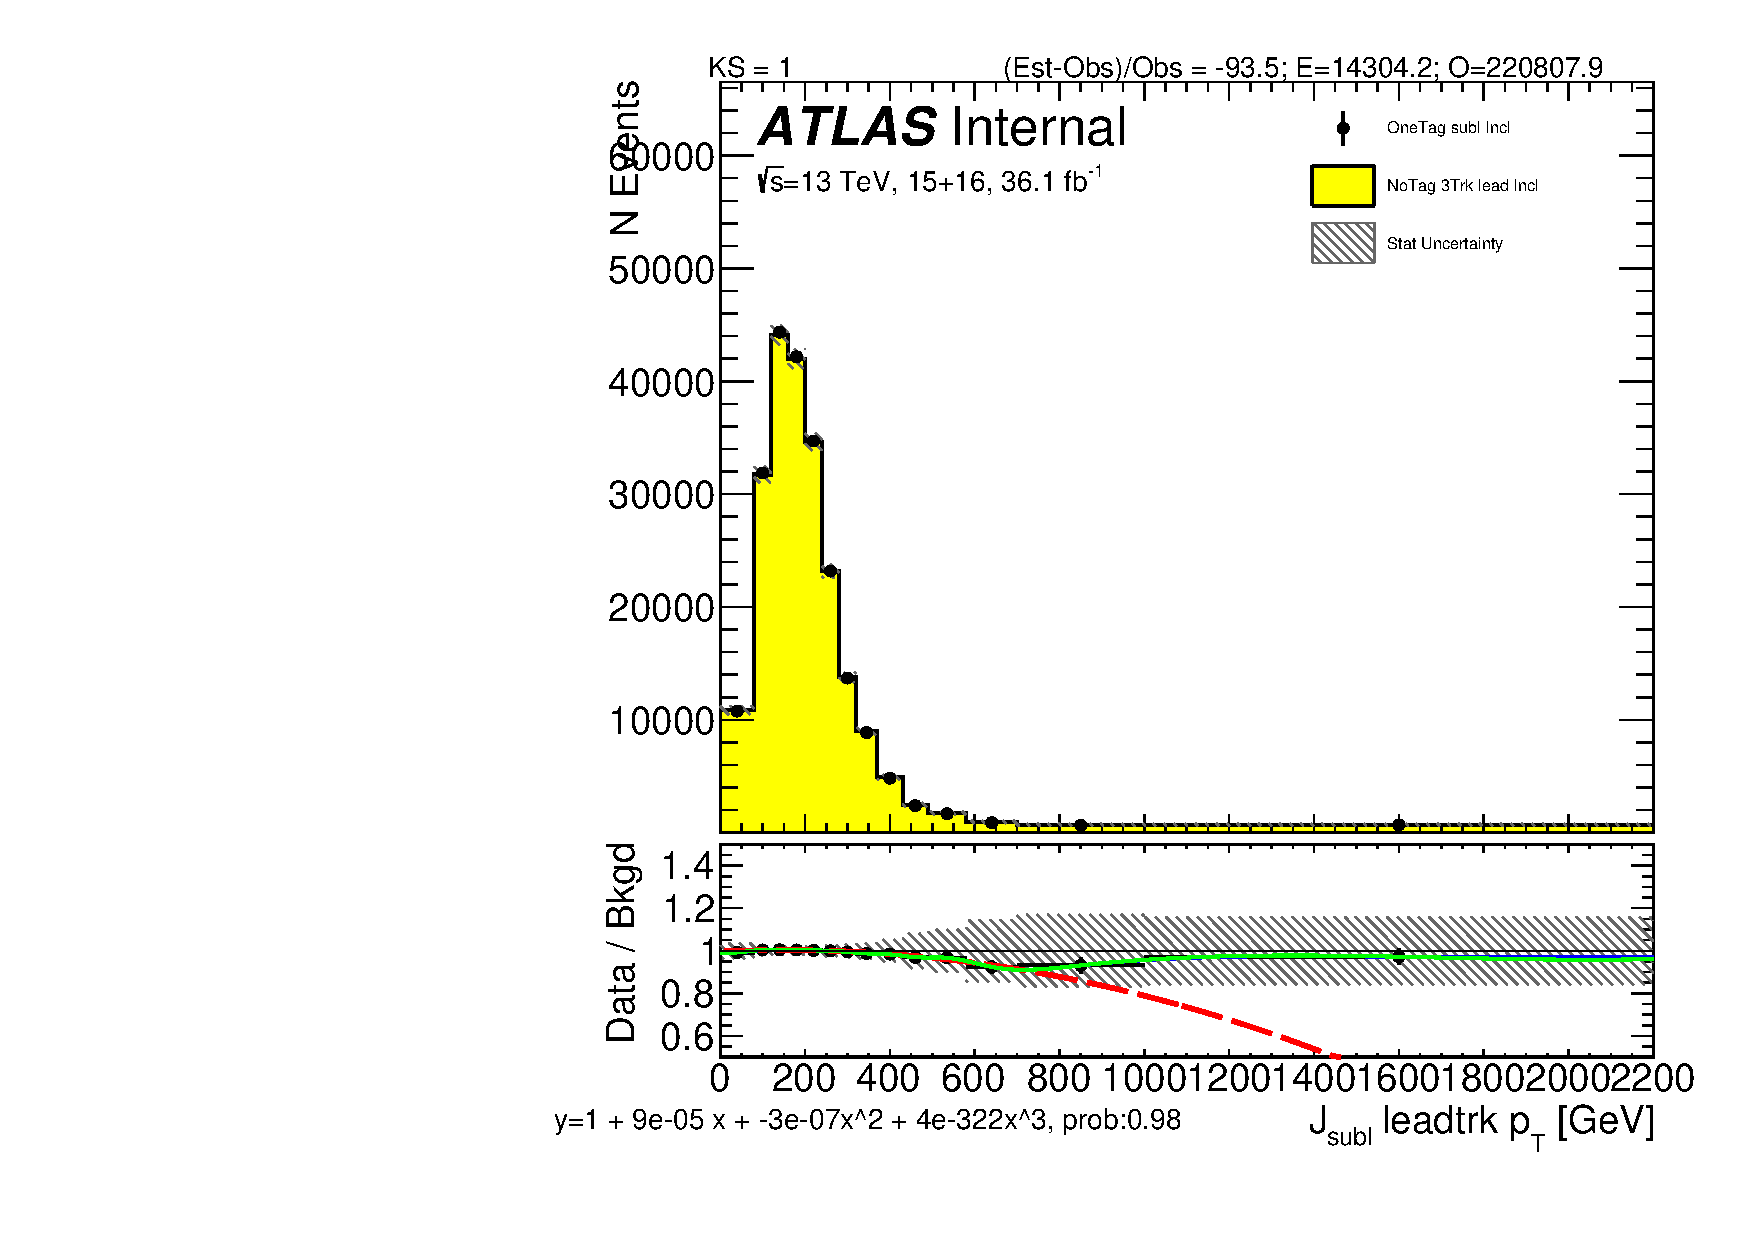
\includegraphics[width=0.32\textwidth,angle=-90]{figures/boosted/Reweight/Fits/Moriond_bkg_3_NoTag_3Trk_lead_Incl_sublHCand_trk0_Pt.pdf}
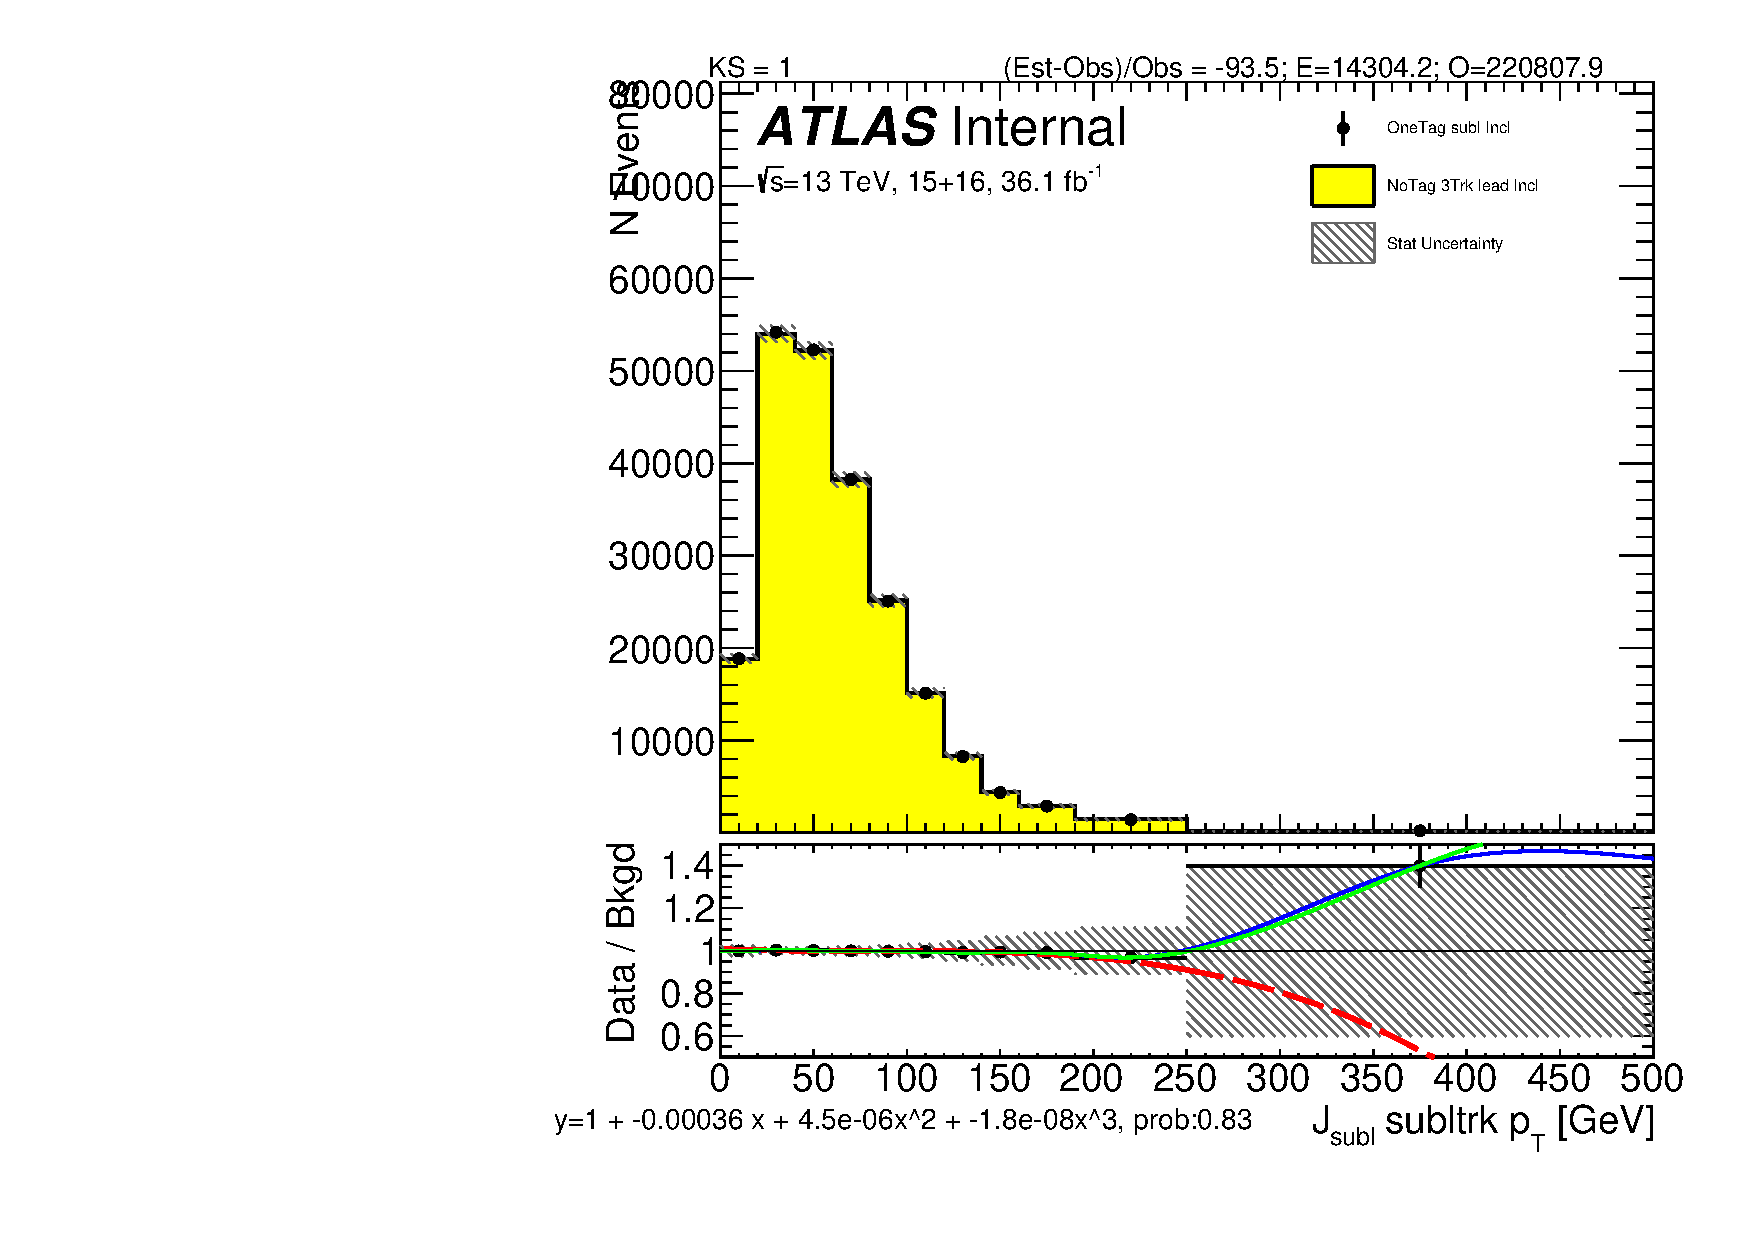
\includegraphics[width=0.32\textwidth,angle=-90]{figures/boosted/Reweight/Fits/Moriond_bkg_3_NoTag_3Trk_lead_Incl_sublHCand_trk1_Pt.pdf} \\
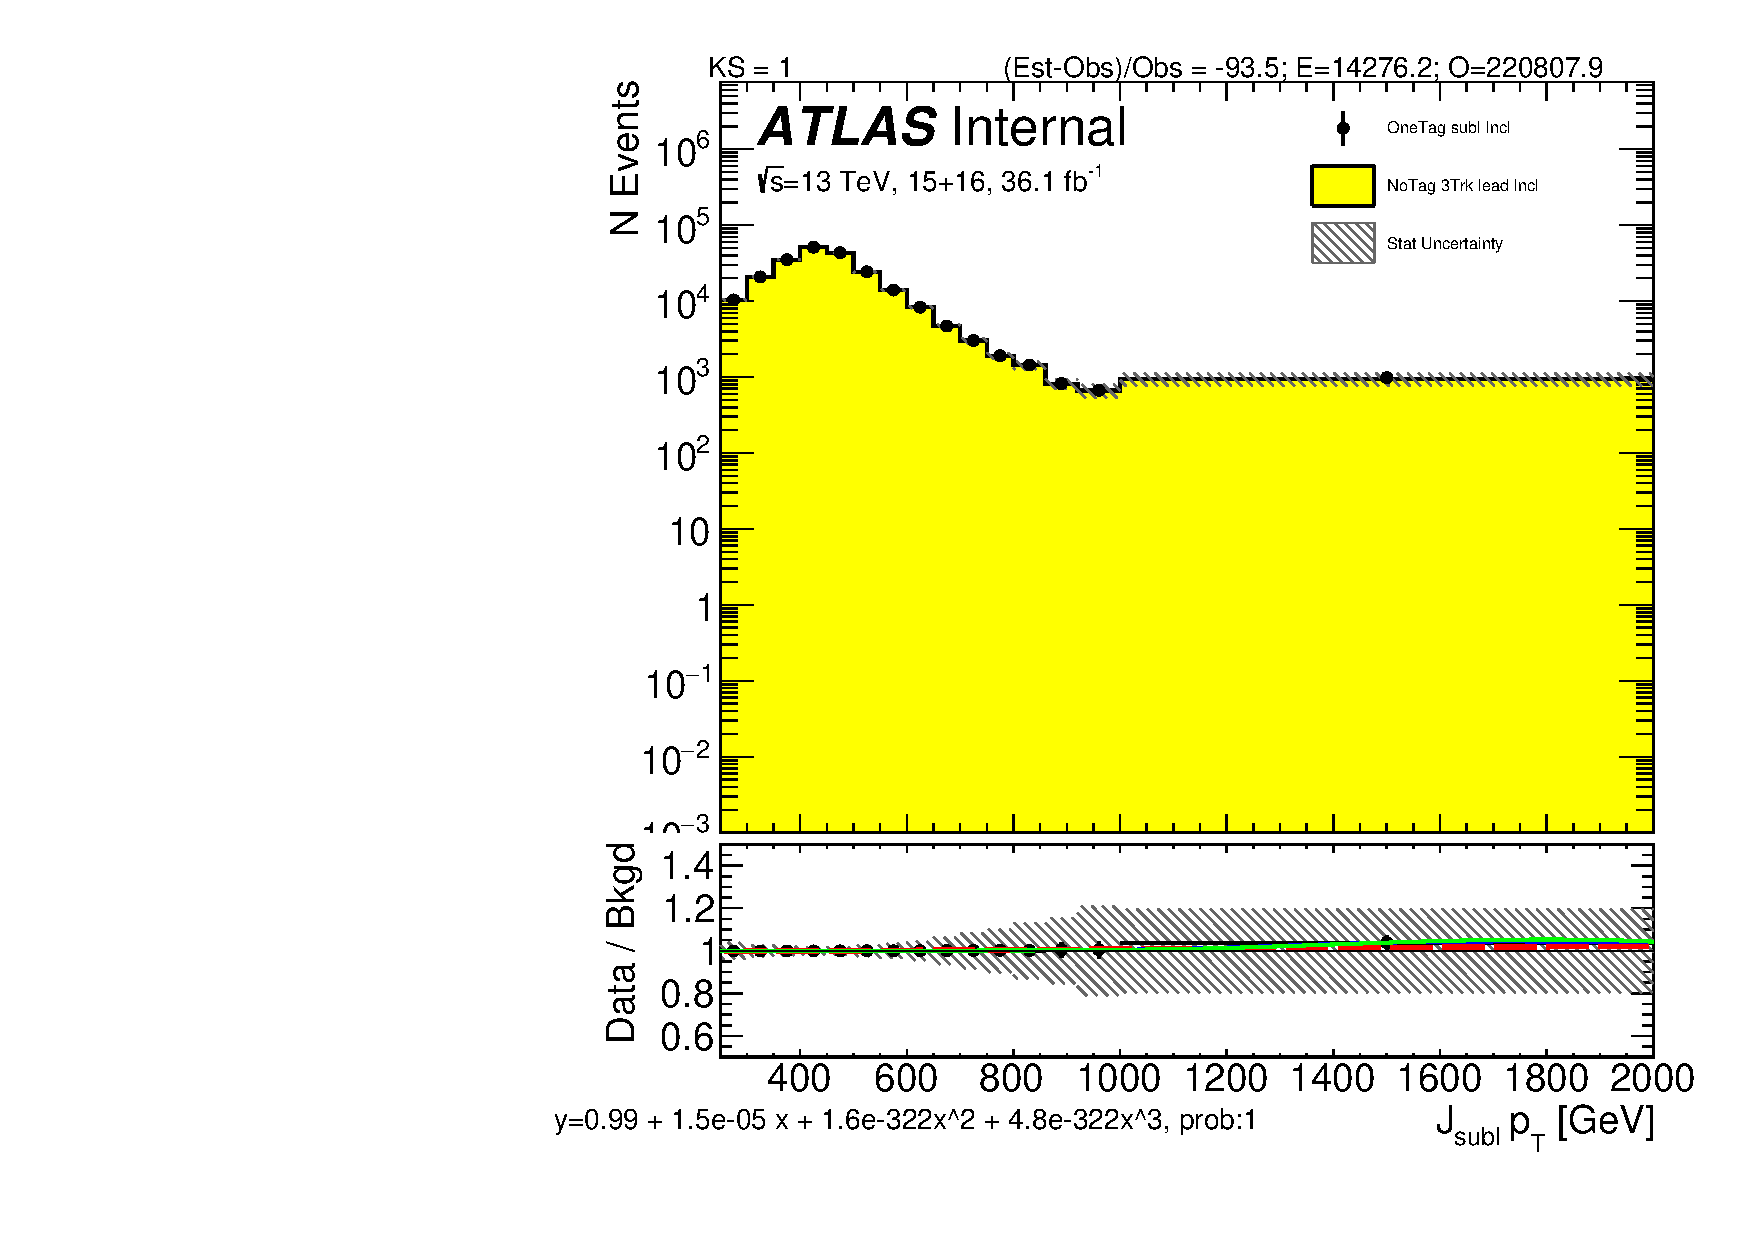
\includegraphics[width=0.32\textwidth,angle=-90]{figures/boosted/Reweight/Fits/Moriond_bkg_9_NoTag_3Trk_lead_Incl_sublHCand_Pt_m_1.pdf}
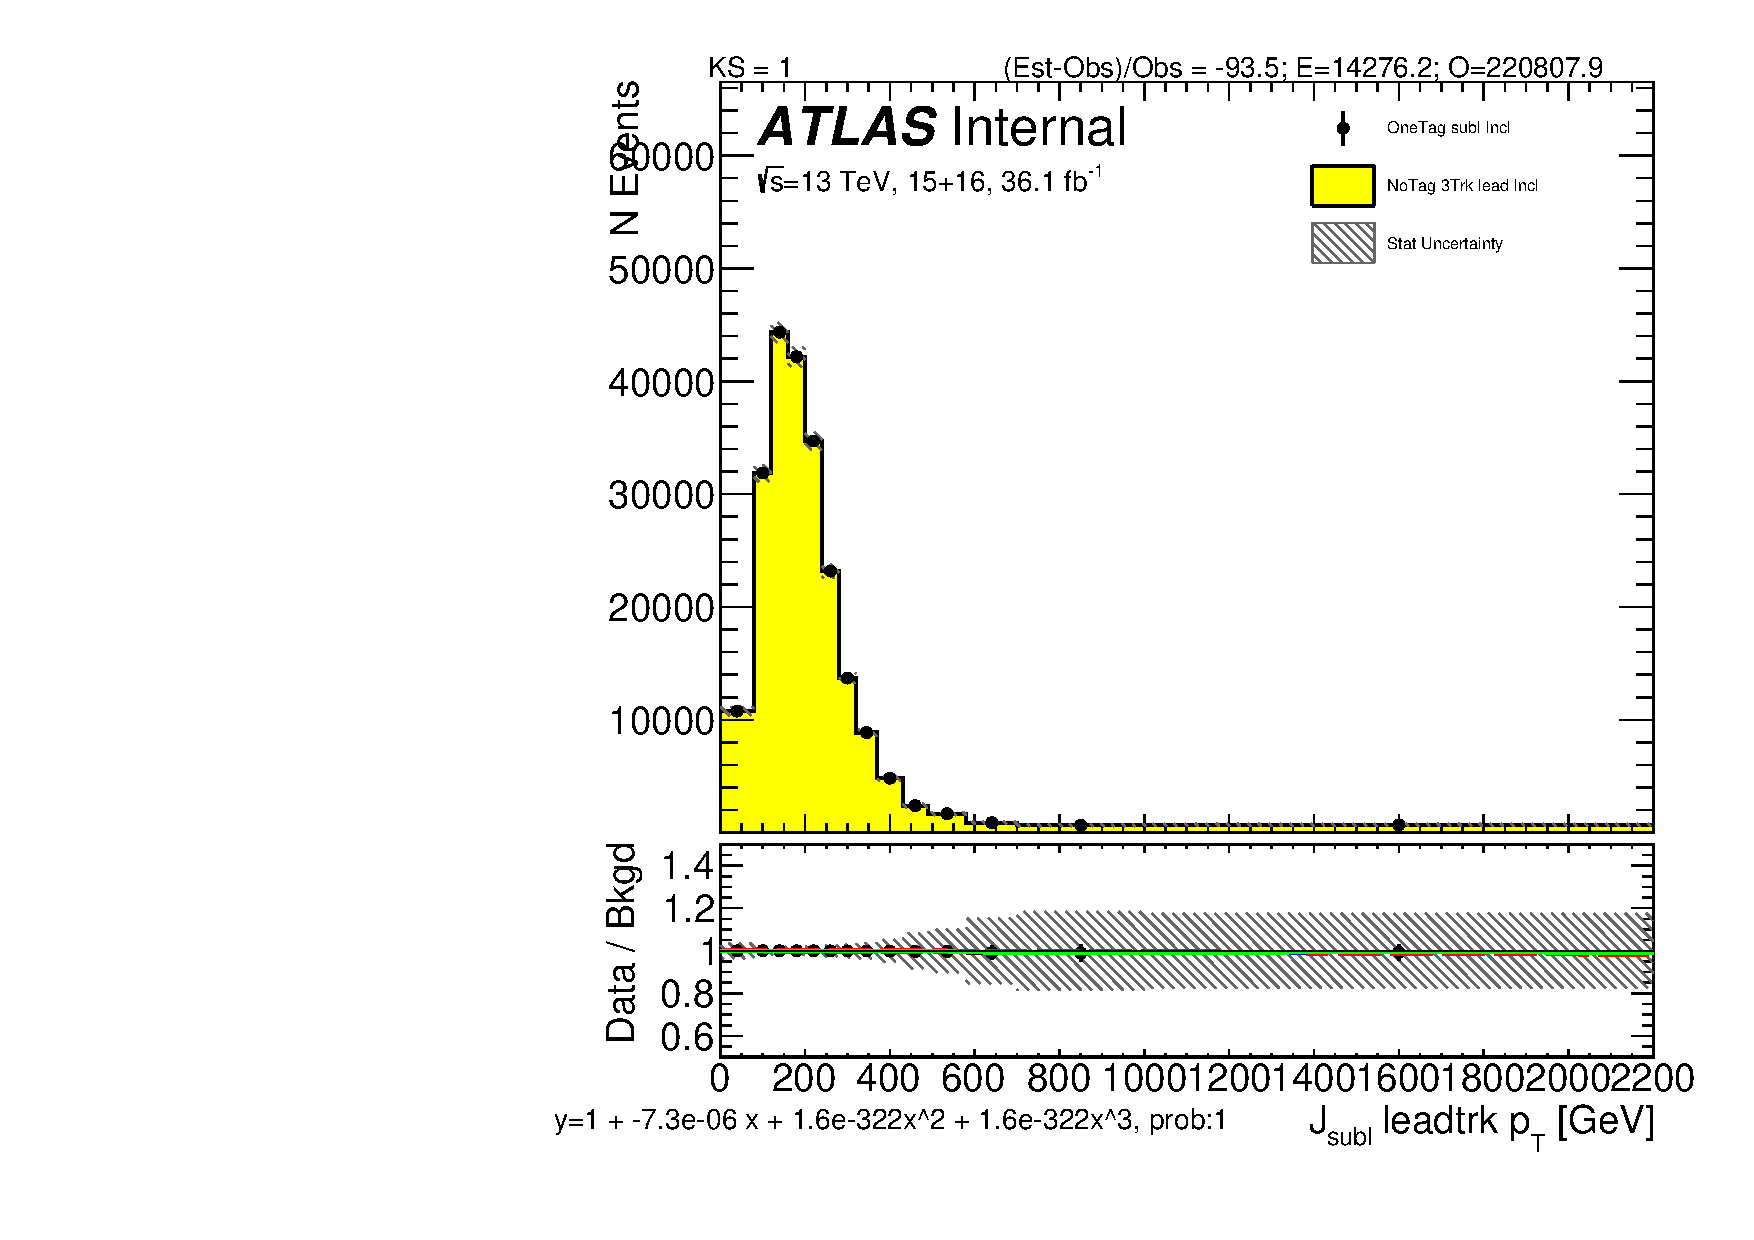
\includegraphics[width=0.32\textwidth,angle=-90]{figures/boosted/Reweight/Fits/Moriond_bkg_9_NoTag_3Trk_lead_Incl_sublHCand_trk0_Pt.pdf}
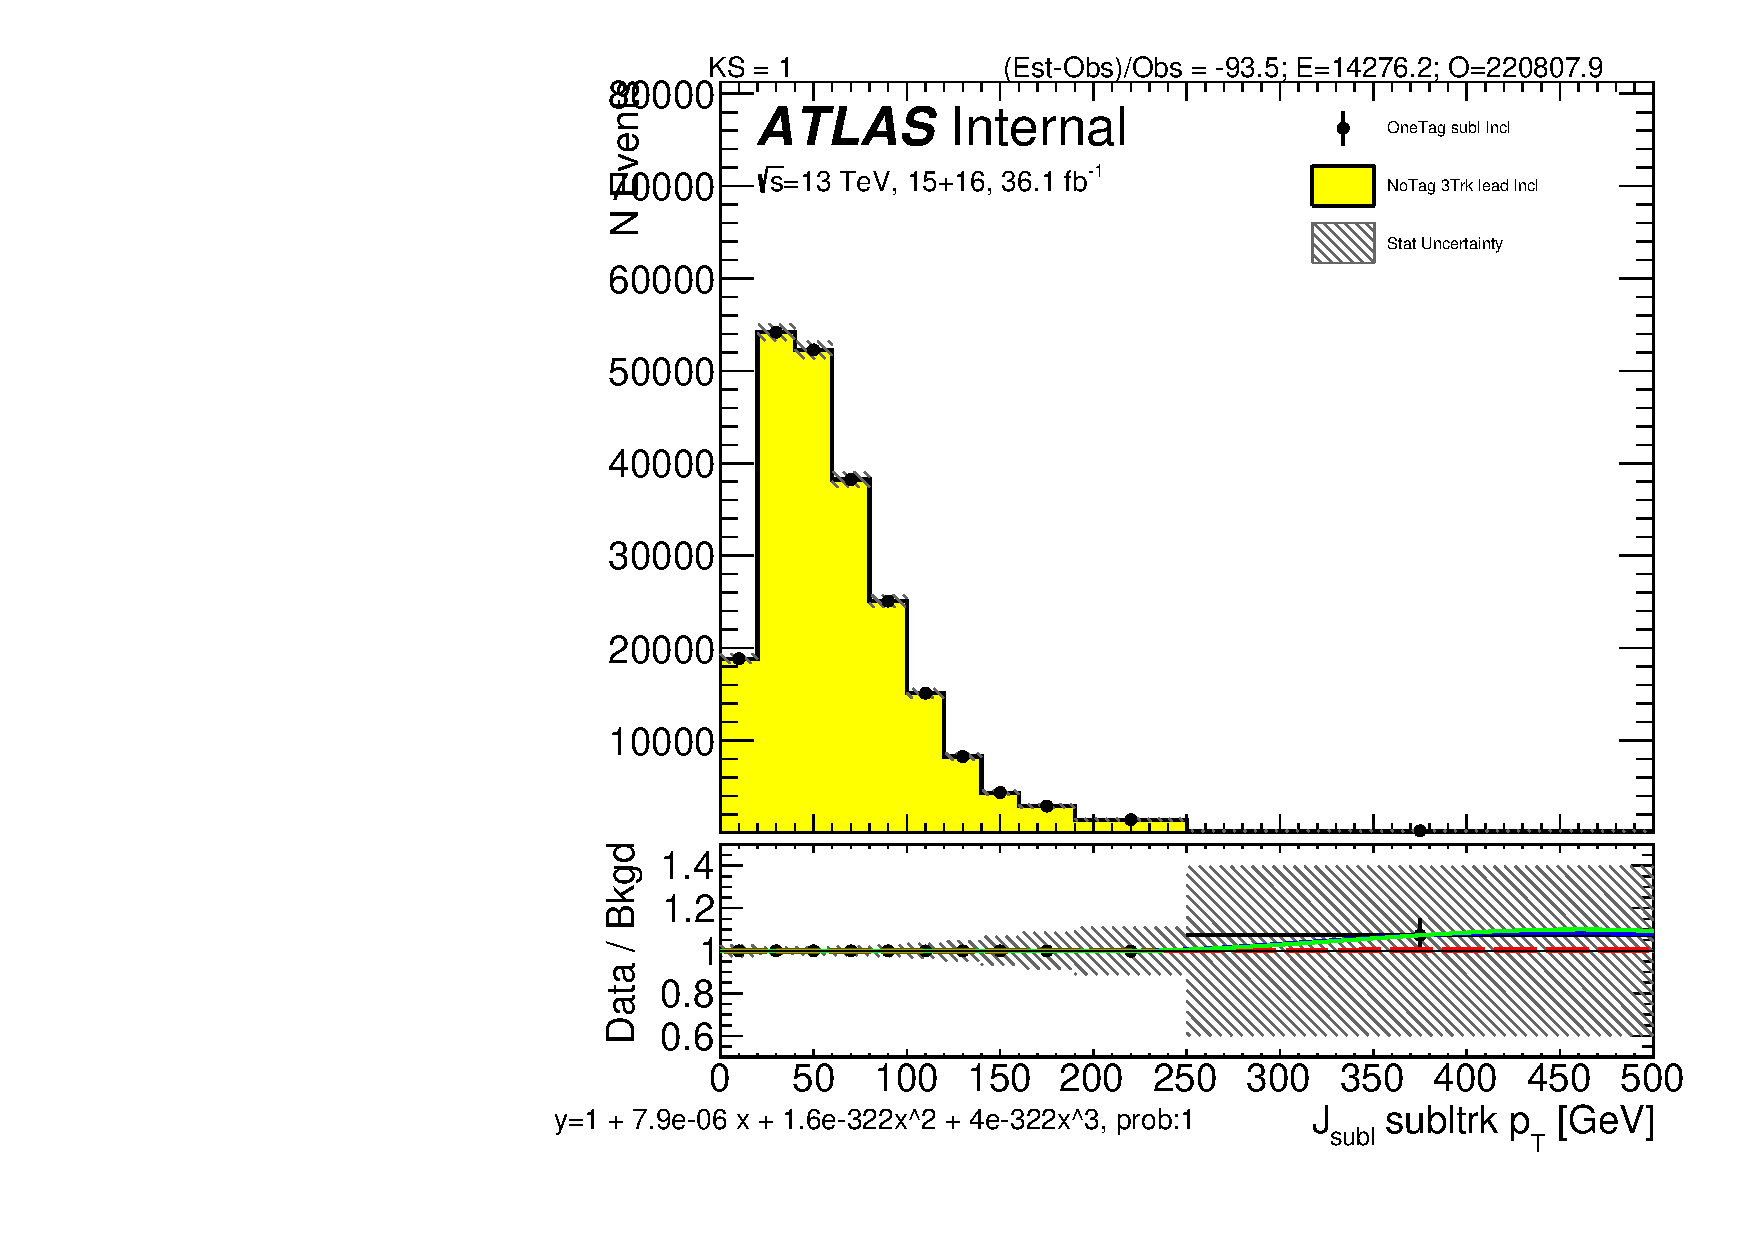
\includegraphics[width=0.32\textwidth,angle=-90]{figures/boosted/Reweight/Fits/Moriond_bkg_9_NoTag_3Trk_lead_Incl_sublHCand_trk1_Pt.pdf} \\
\caption{For $3b$ background estimate: the fits to the ratio of the data in the $2b$ category, of the sublleading Higgs candidate $2b$-tagged events's subleading Higgs candidate distributions(black point), over the leading Higgs candidate $1b$-tagged events's subleading Higgs candidate distributions(yellow). Distributions and fits to the estimated QCD background for large-$R$ jet $p_{T}$ (left),  the large-$R$ jet's leading trackjet $p_T$ (middle), and large-$R$ jet's subleading trackjet $p_T$ (right) are shown.  Figure are shown before reweighting (top row), after the first iteration(second row), after the fourth iteration(third row), and after the last iteration (bottow row). The green line is the spline extrapolation; and the red line is a polynomial fit.}
\label{fig:rw-3b-lead}
\end{center}
\end{figure*}

\begin{figure*}[htbp!]
\begin{center}
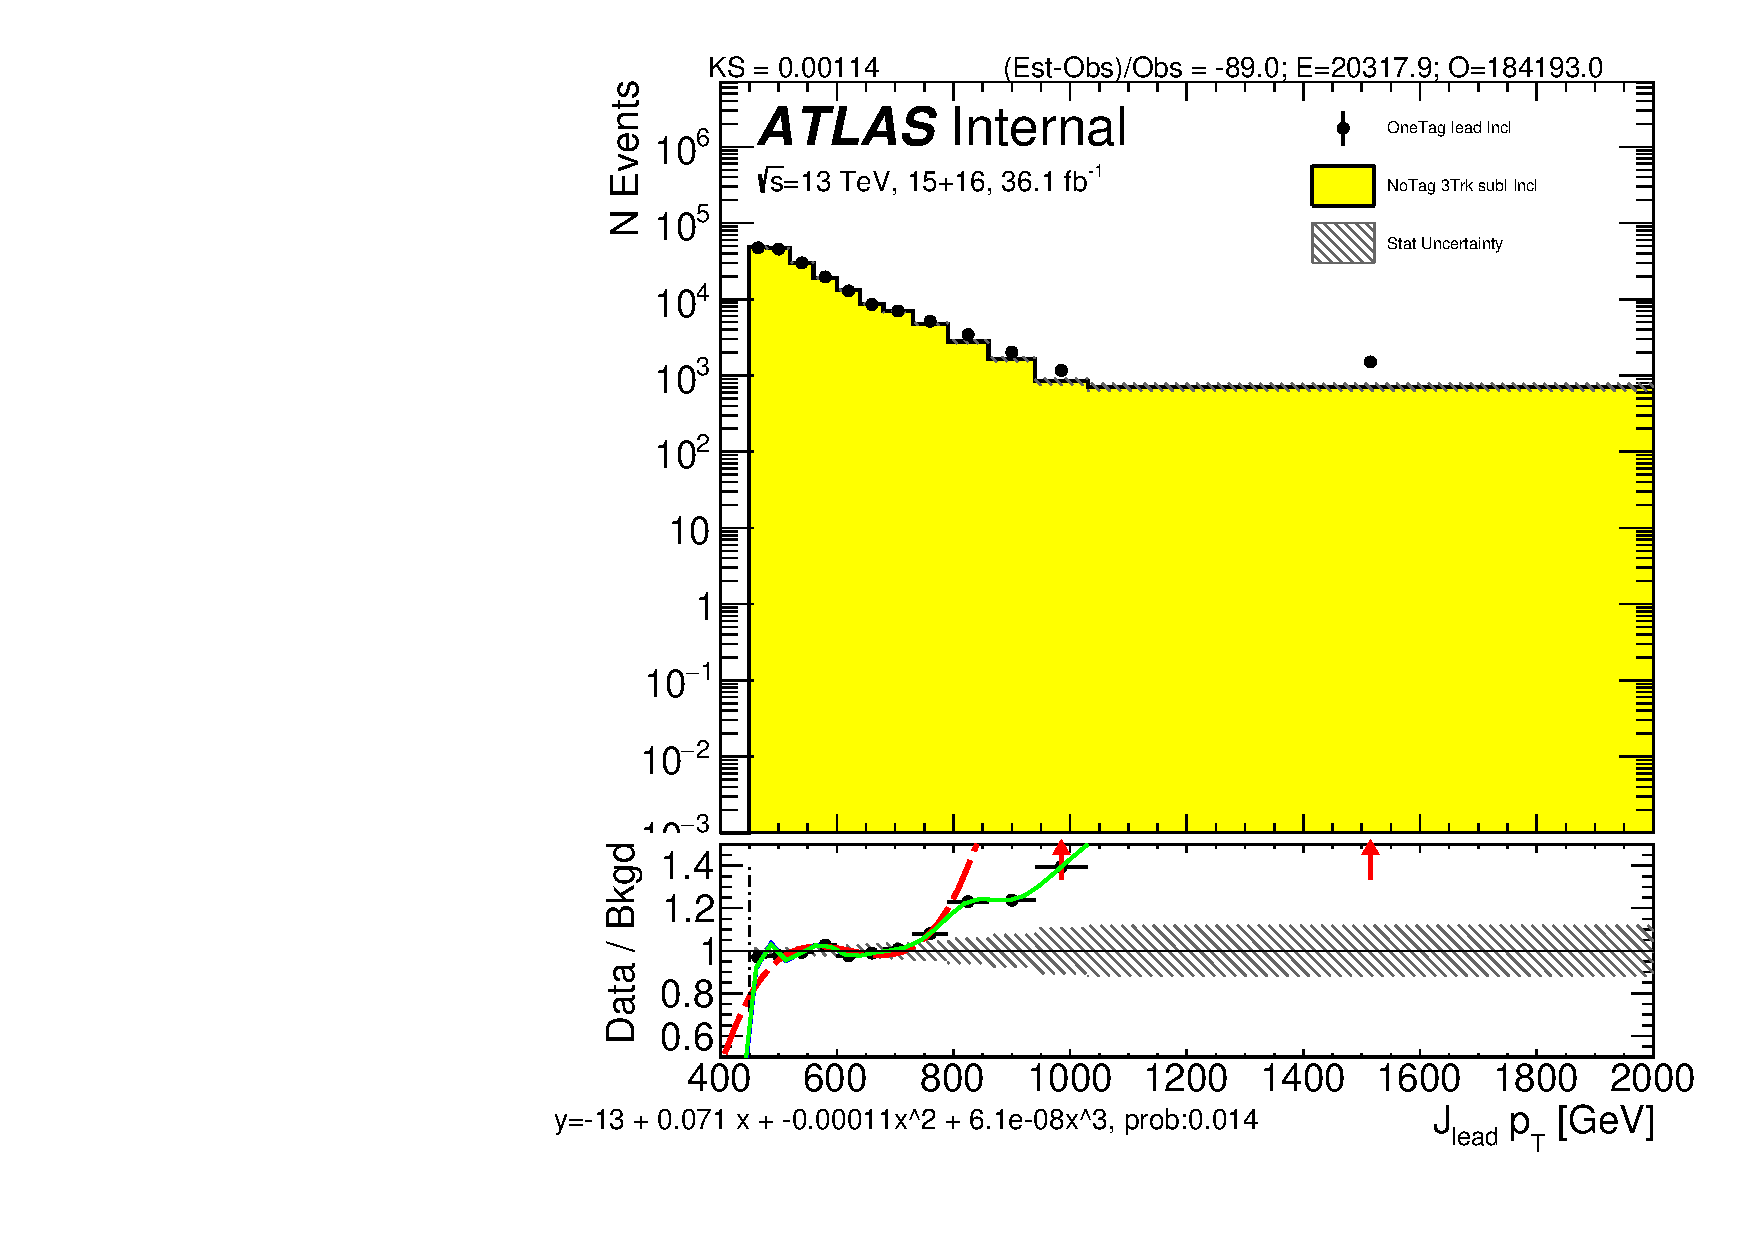
\includegraphics[width=0.32\textwidth,angle=-90]{figures/boosted/Reweight/Fits/Moriond_NoTag_3Trk_subl_Incl_leadHCand_Pt_m_1.pdf}
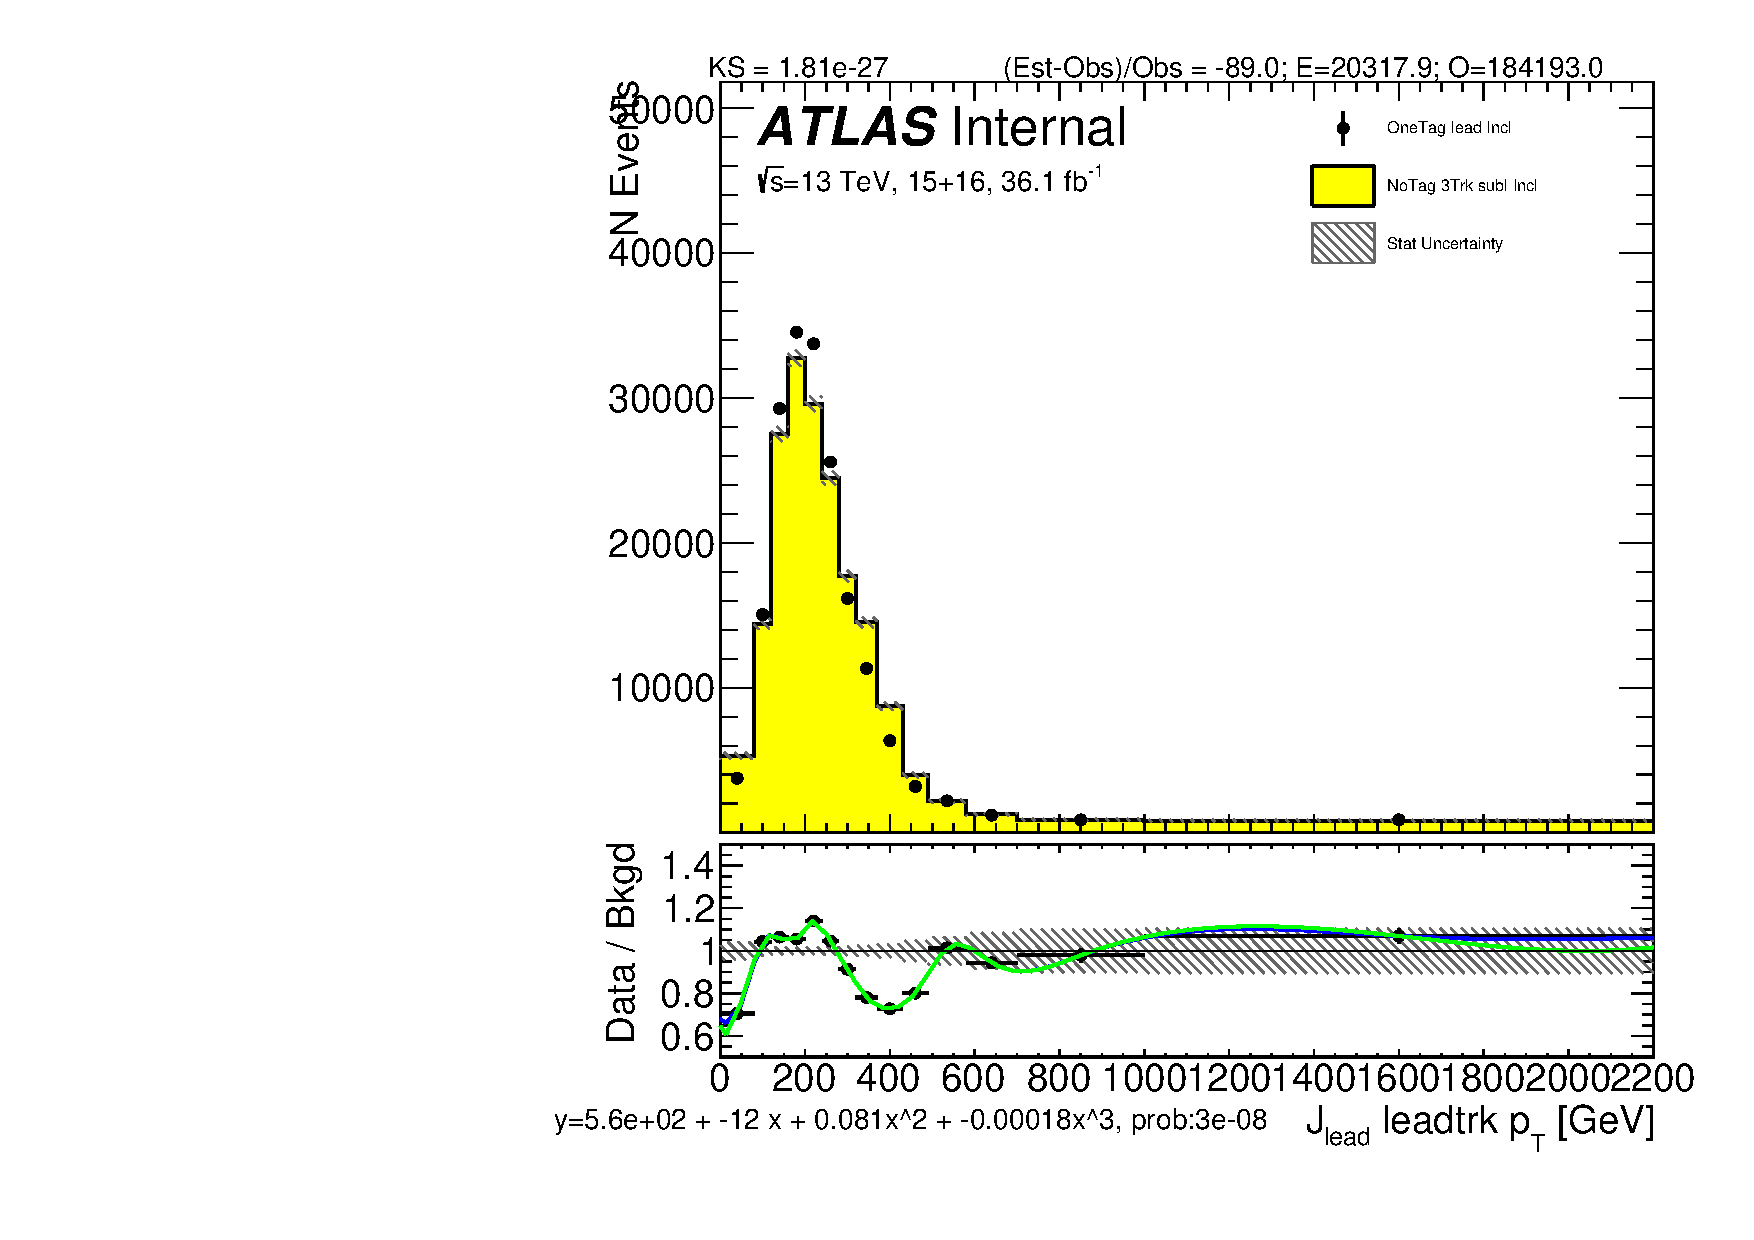
\includegraphics[width=0.32\textwidth,angle=-90]{figures/boosted/Reweight/Fits/Moriond_NoTag_3Trk_subl_Incl_leadHCand_trk0_Pt.pdf}
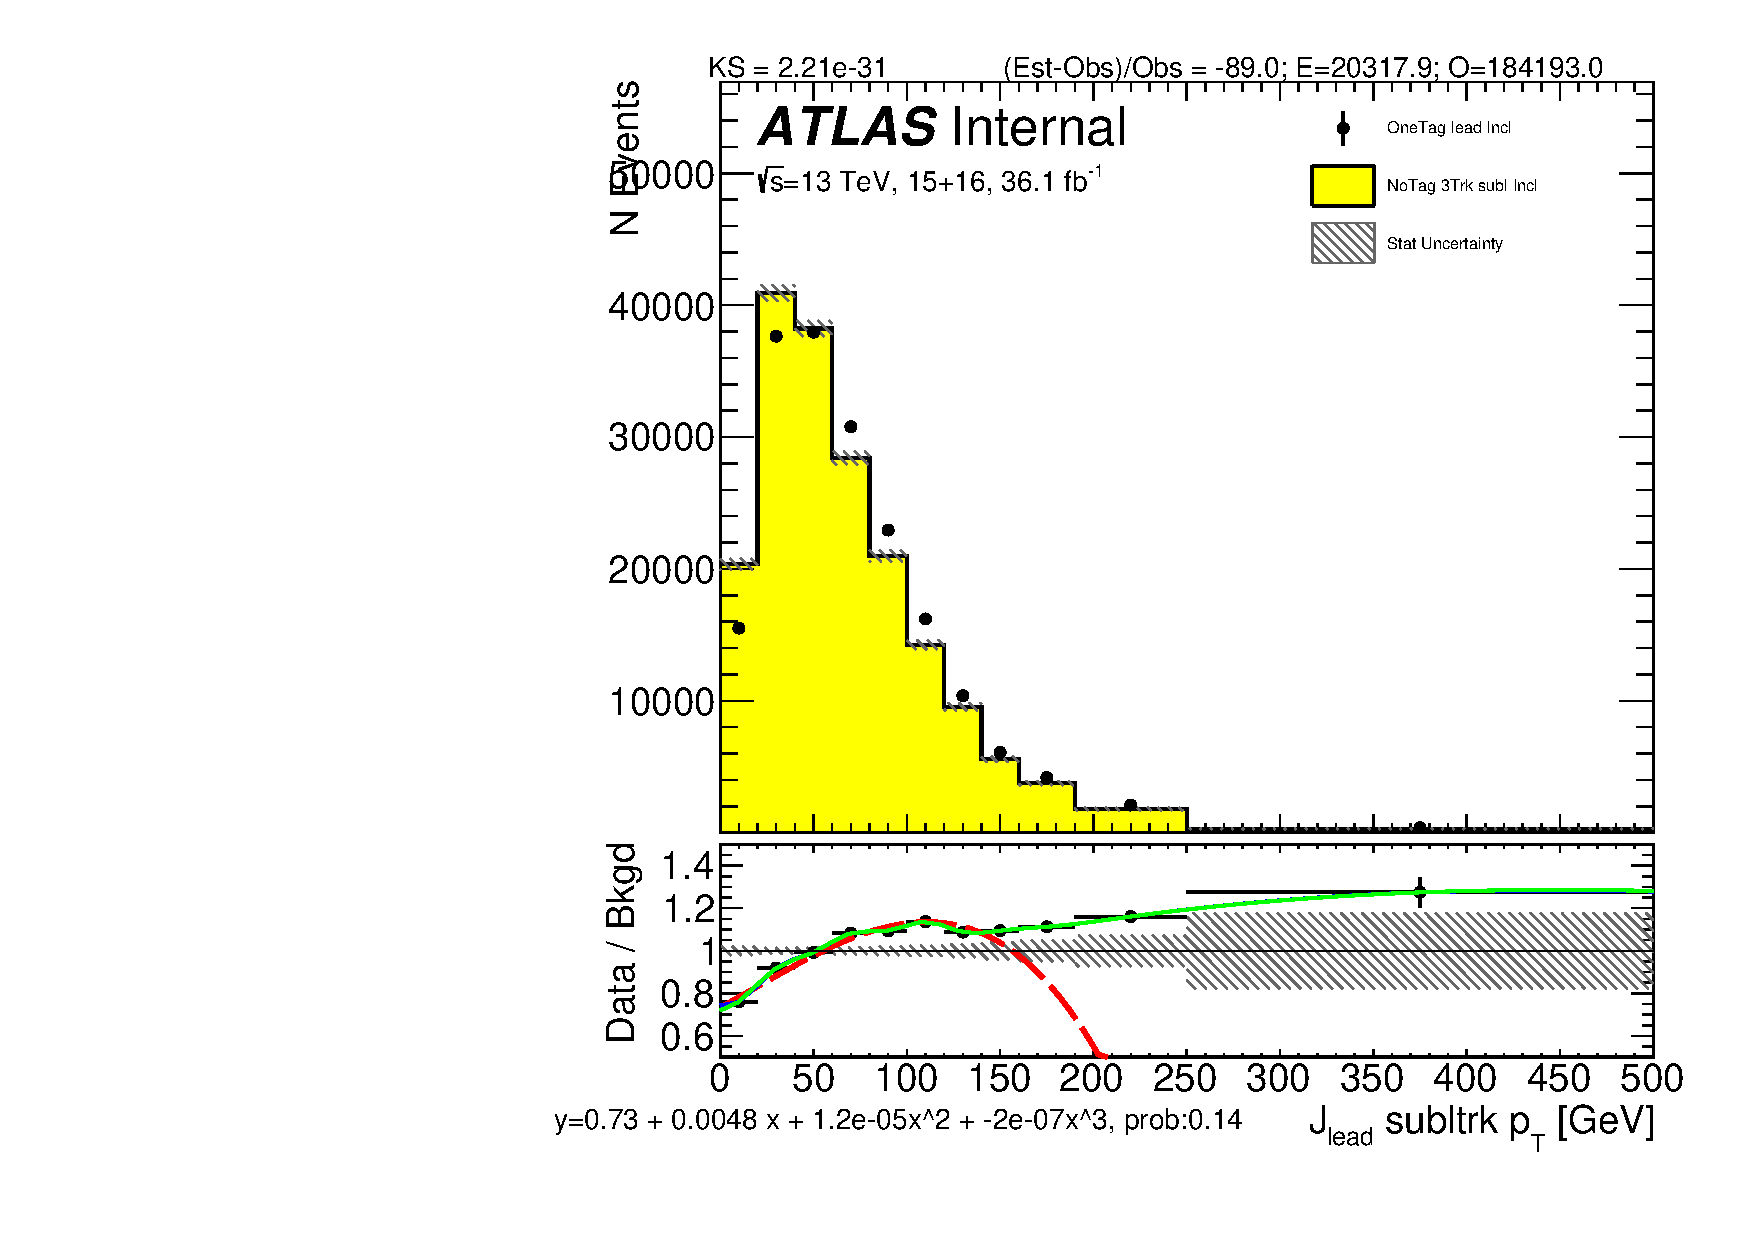
\includegraphics[width=0.32\textwidth,angle=-90]{figures/boosted/Reweight/Fits/Moriond_NoTag_3Trk_subl_Incl_leadHCand_trk1_Pt.pdf} \\
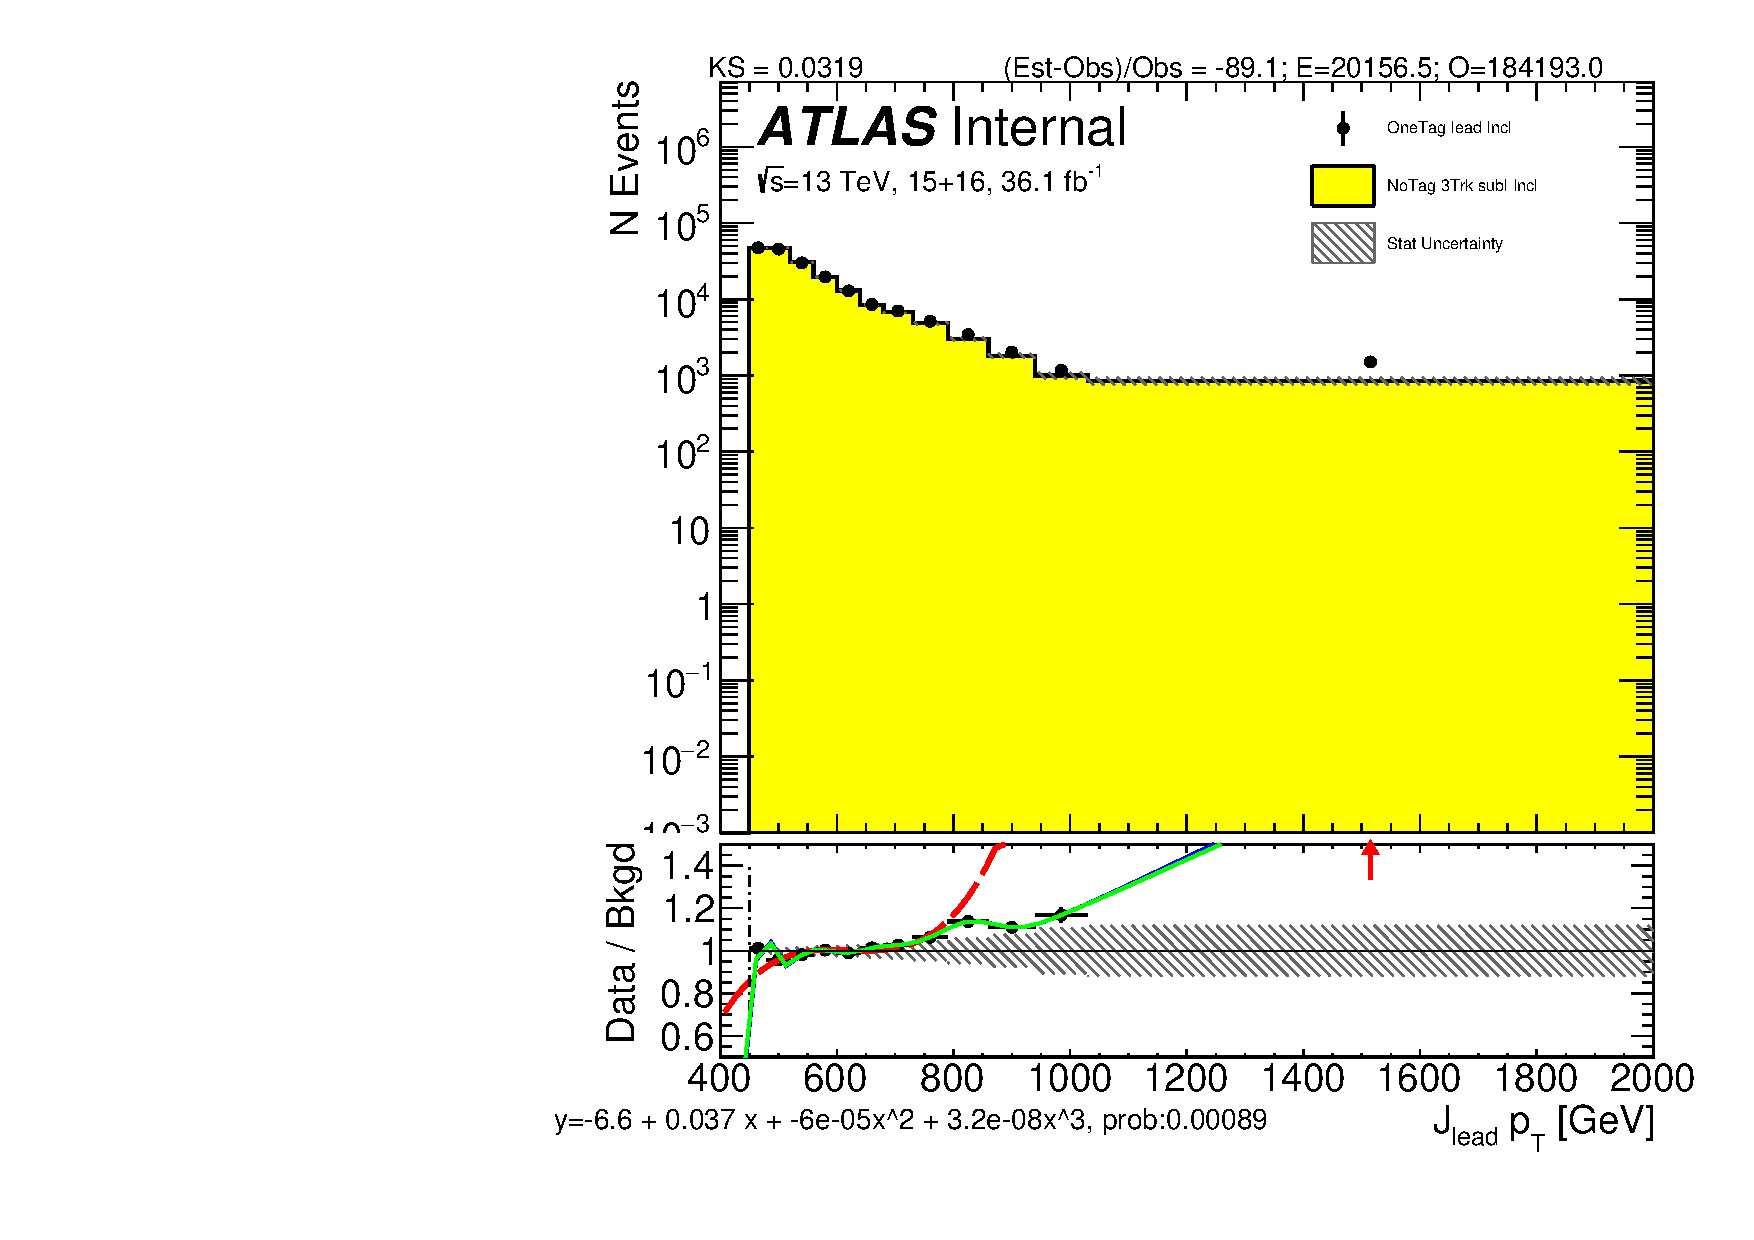
\includegraphics[width=0.32\textwidth,angle=-90]{figures/boosted/Reweight/Fits/Moriond_bkg_0_NoTag_3Trk_subl_Incl_leadHCand_Pt_m_1.pdf}
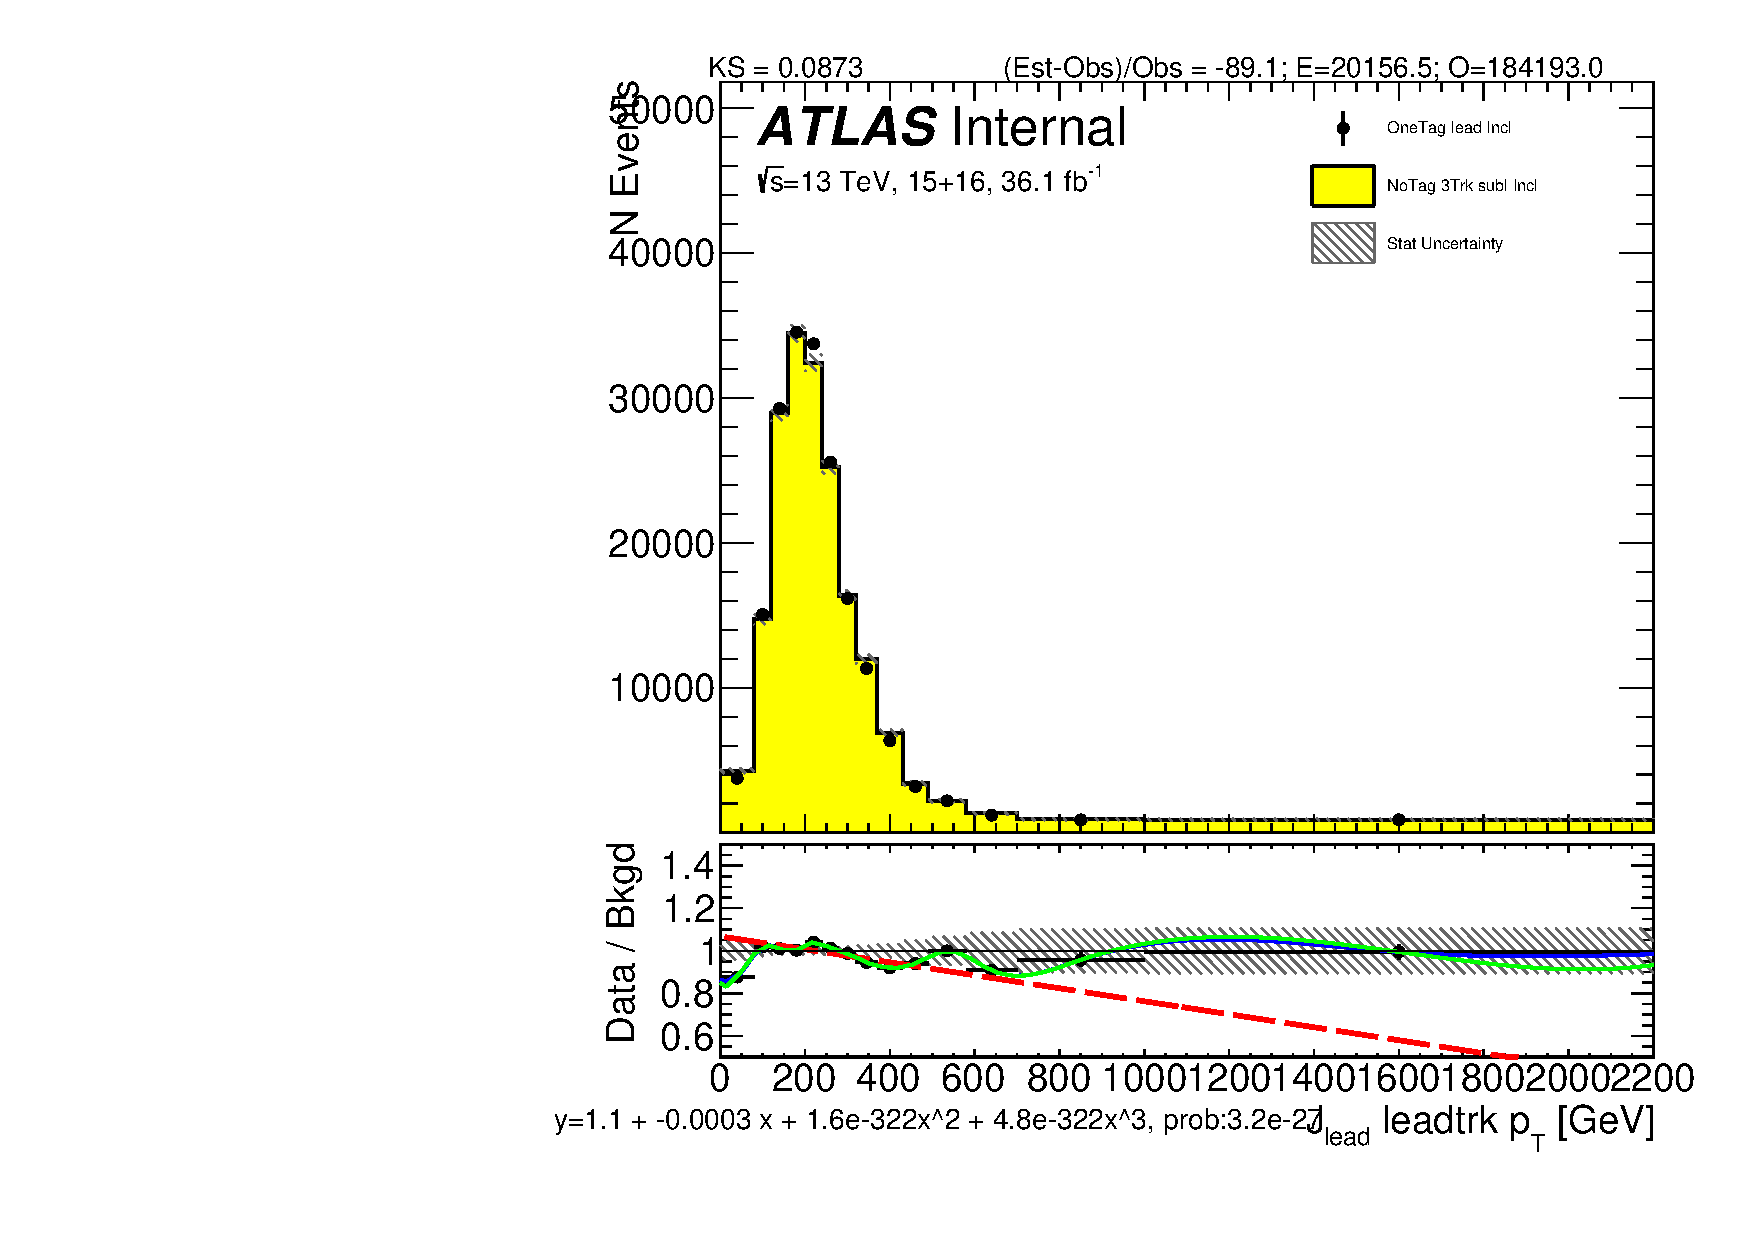
\includegraphics[width=0.32\textwidth,angle=-90]{figures/boosted/Reweight/Fits/Moriond_bkg_0_NoTag_3Trk_subl_Incl_leadHCand_trk0_Pt.pdf}
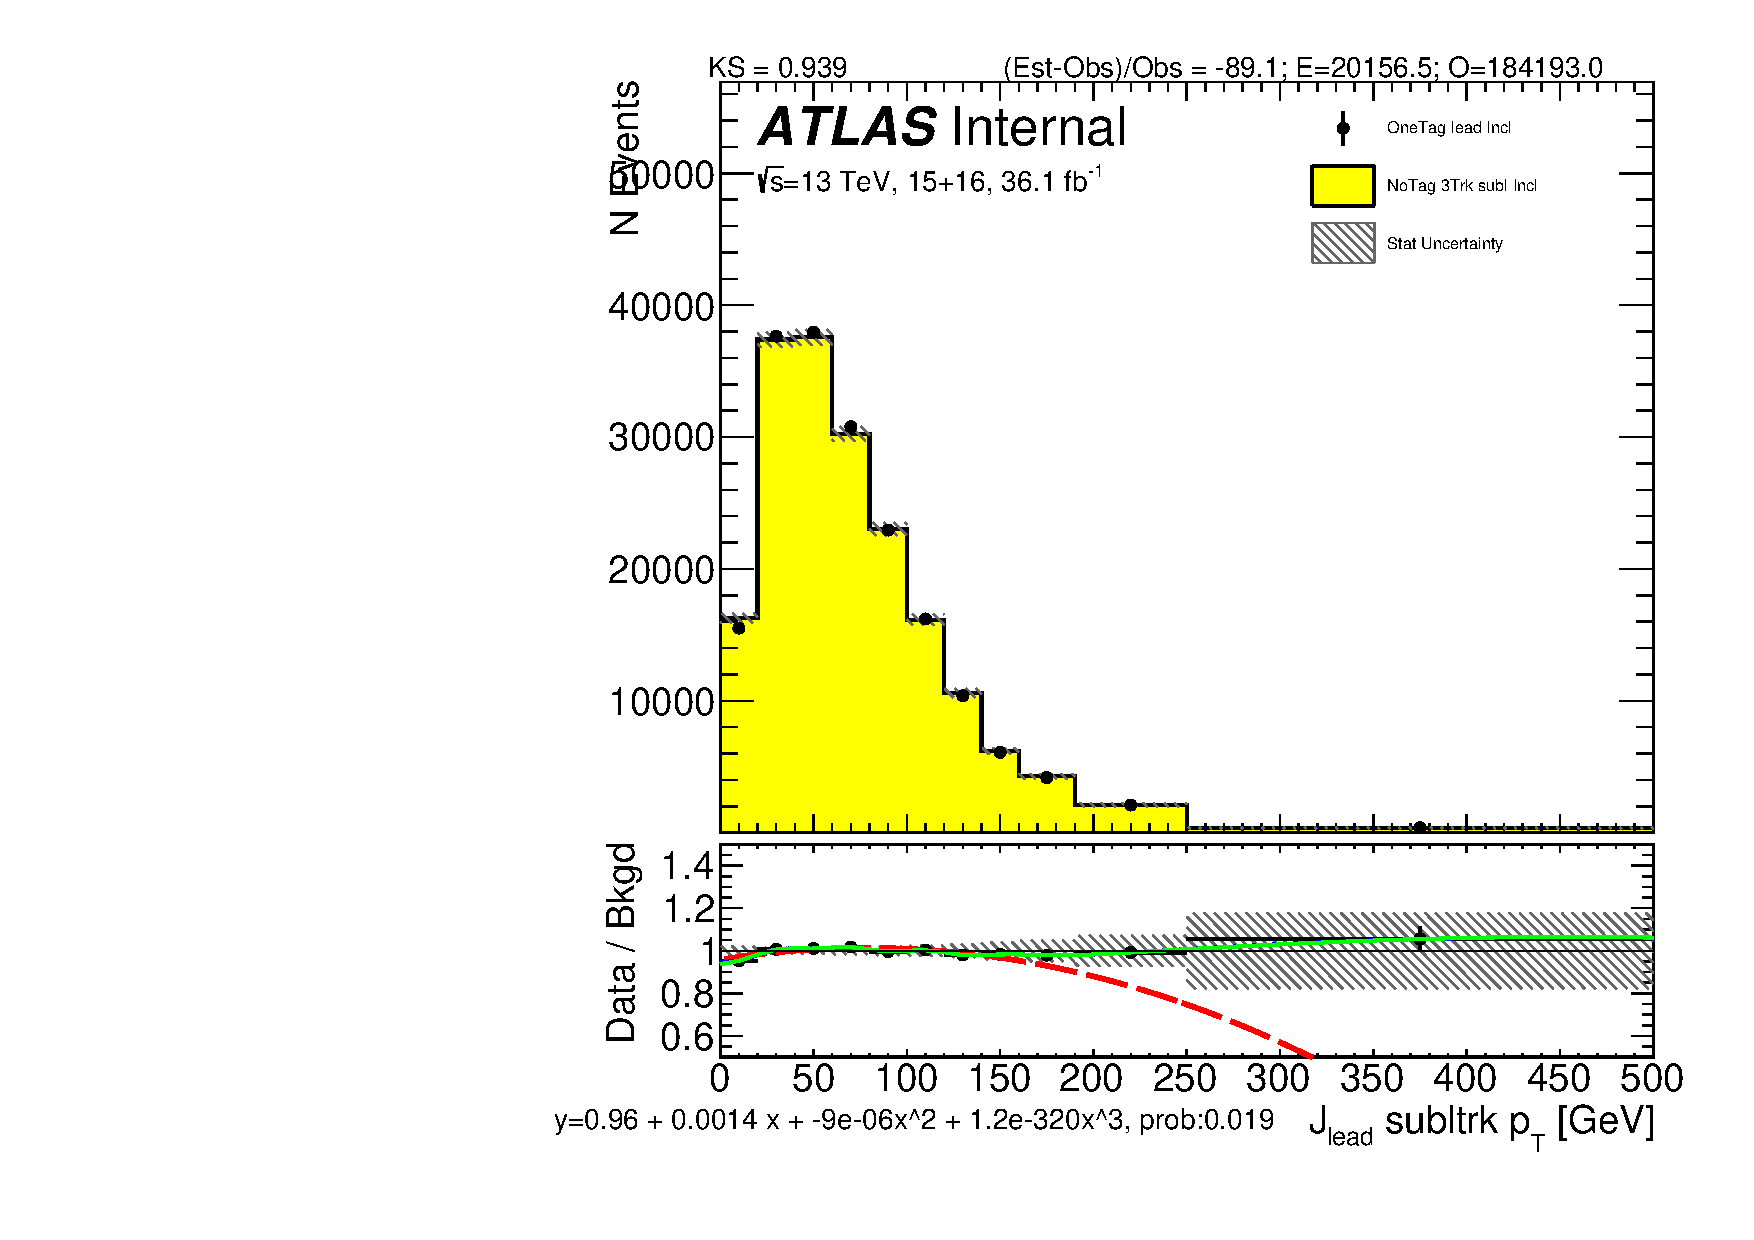
\includegraphics[width=0.32\textwidth,angle=-90]{figures/boosted/Reweight/Fits/Moriond_bkg_0_NoTag_3Trk_subl_Incl_leadHCand_trk1_Pt.pdf} \\
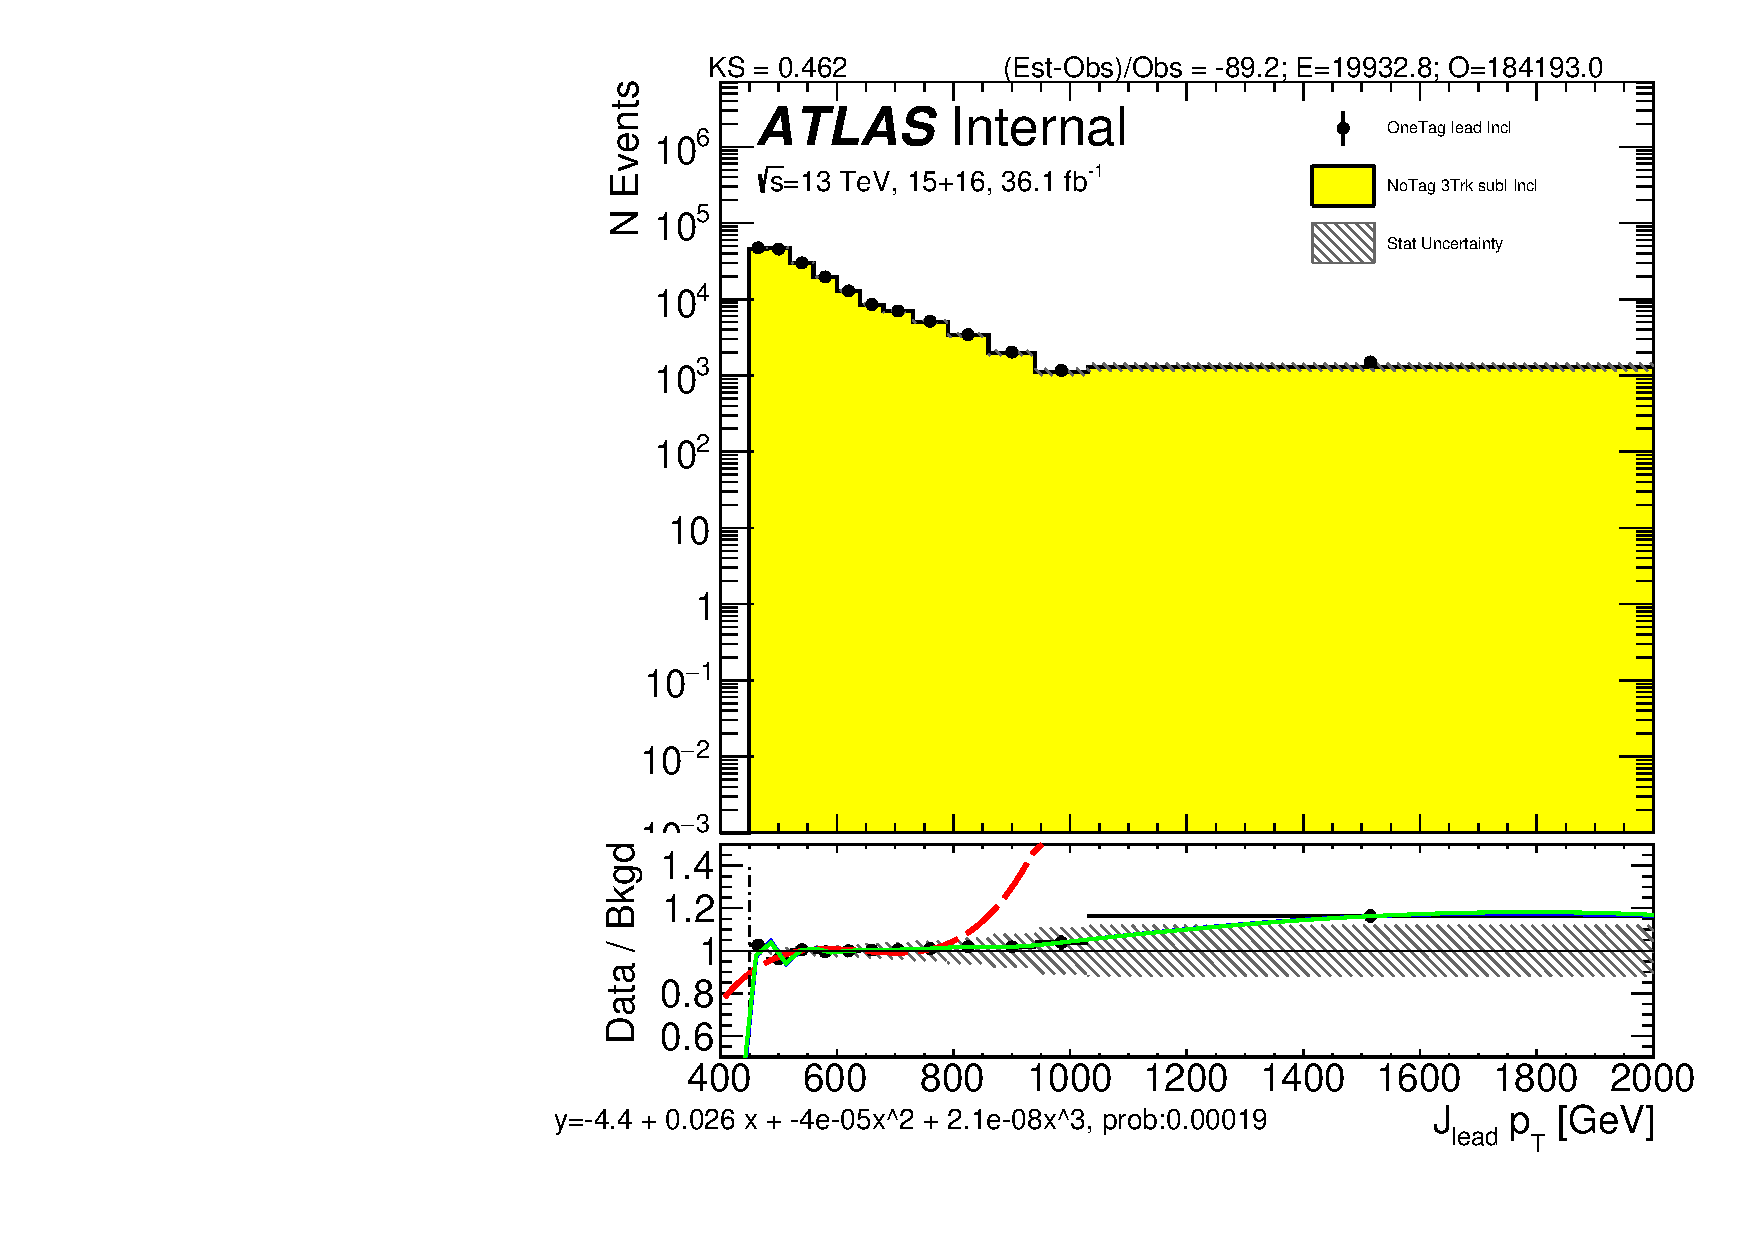
\includegraphics[width=0.32\textwidth,angle=-90]{figures/boosted/Reweight/Fits/Moriond_bkg_3_NoTag_3Trk_subl_Incl_leadHCand_Pt_m_1.pdf}
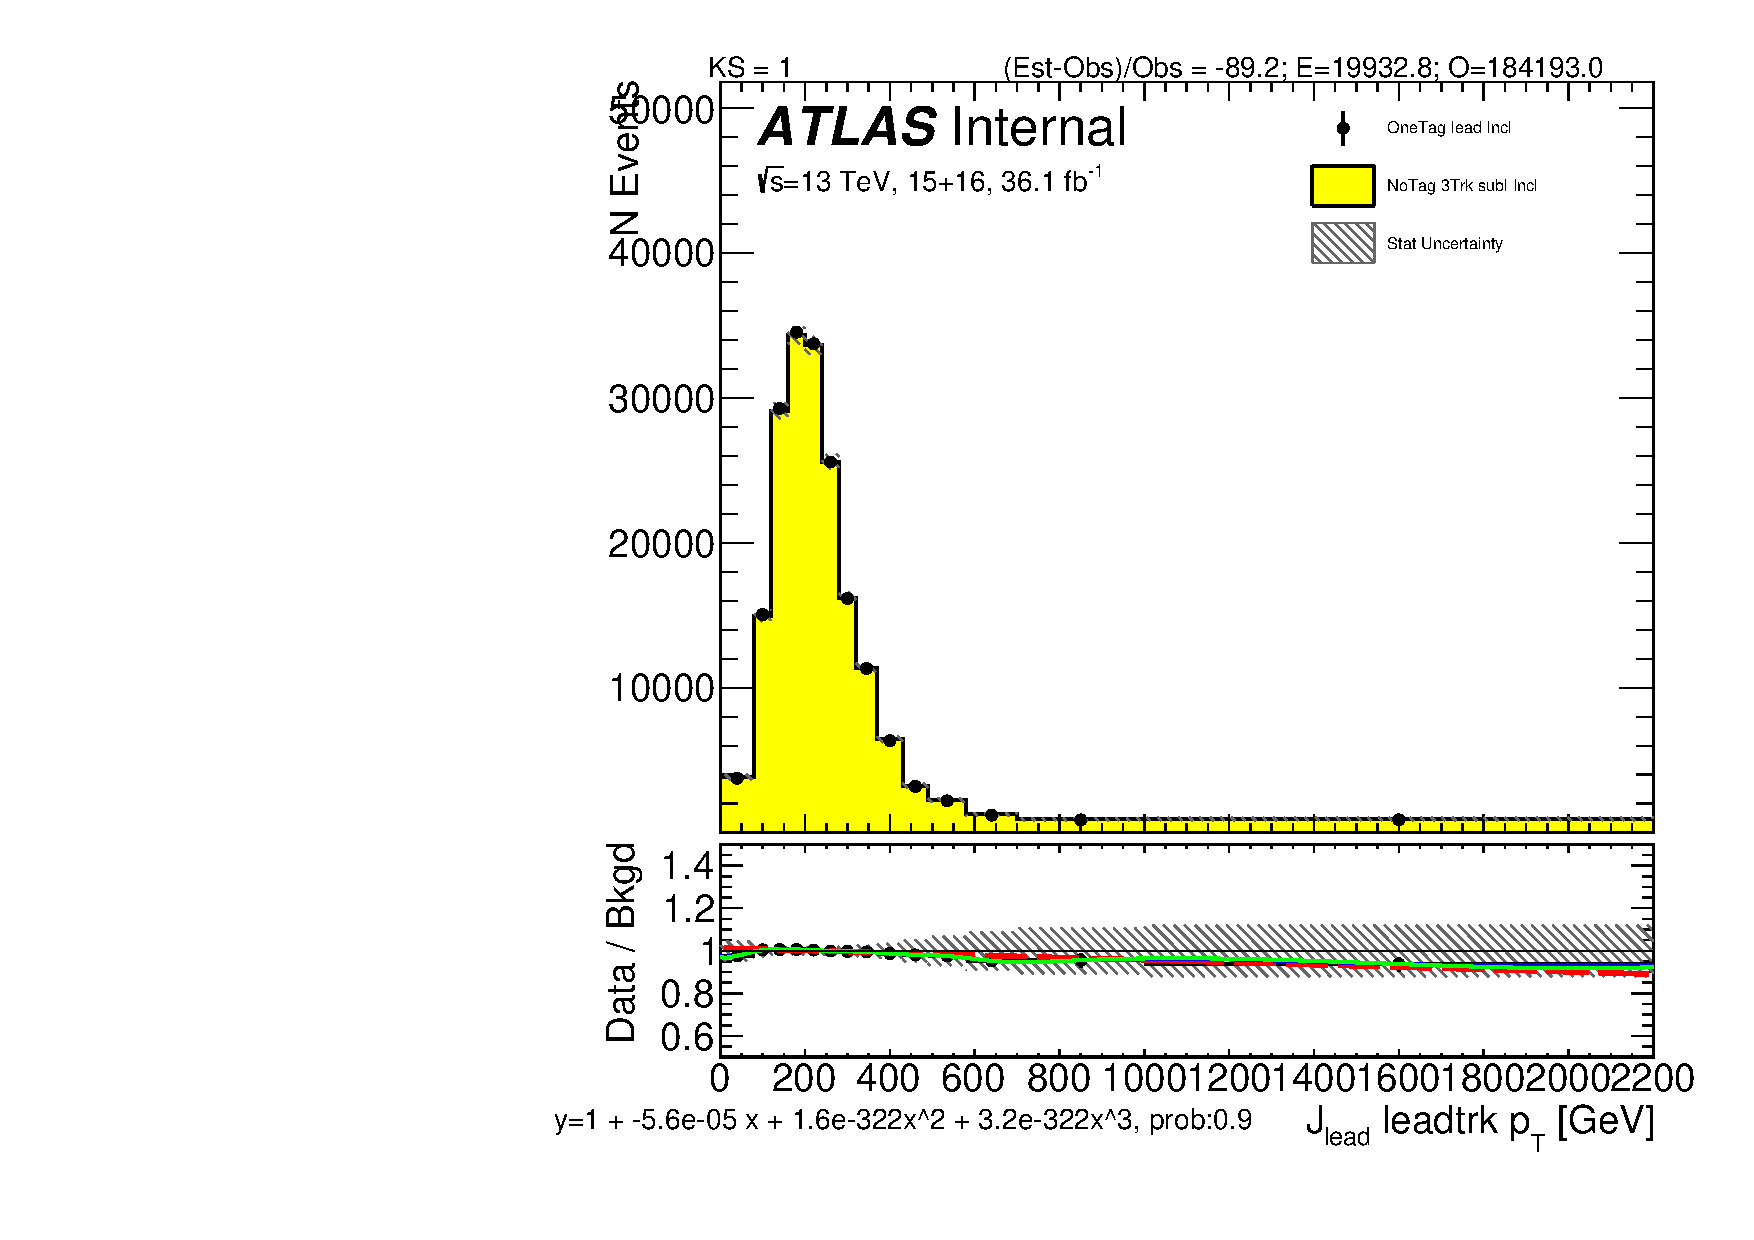
\includegraphics[width=0.32\textwidth,angle=-90]{figures/boosted/Reweight/Fits/Moriond_bkg_3_NoTag_3Trk_subl_Incl_leadHCand_trk0_Pt.pdf}
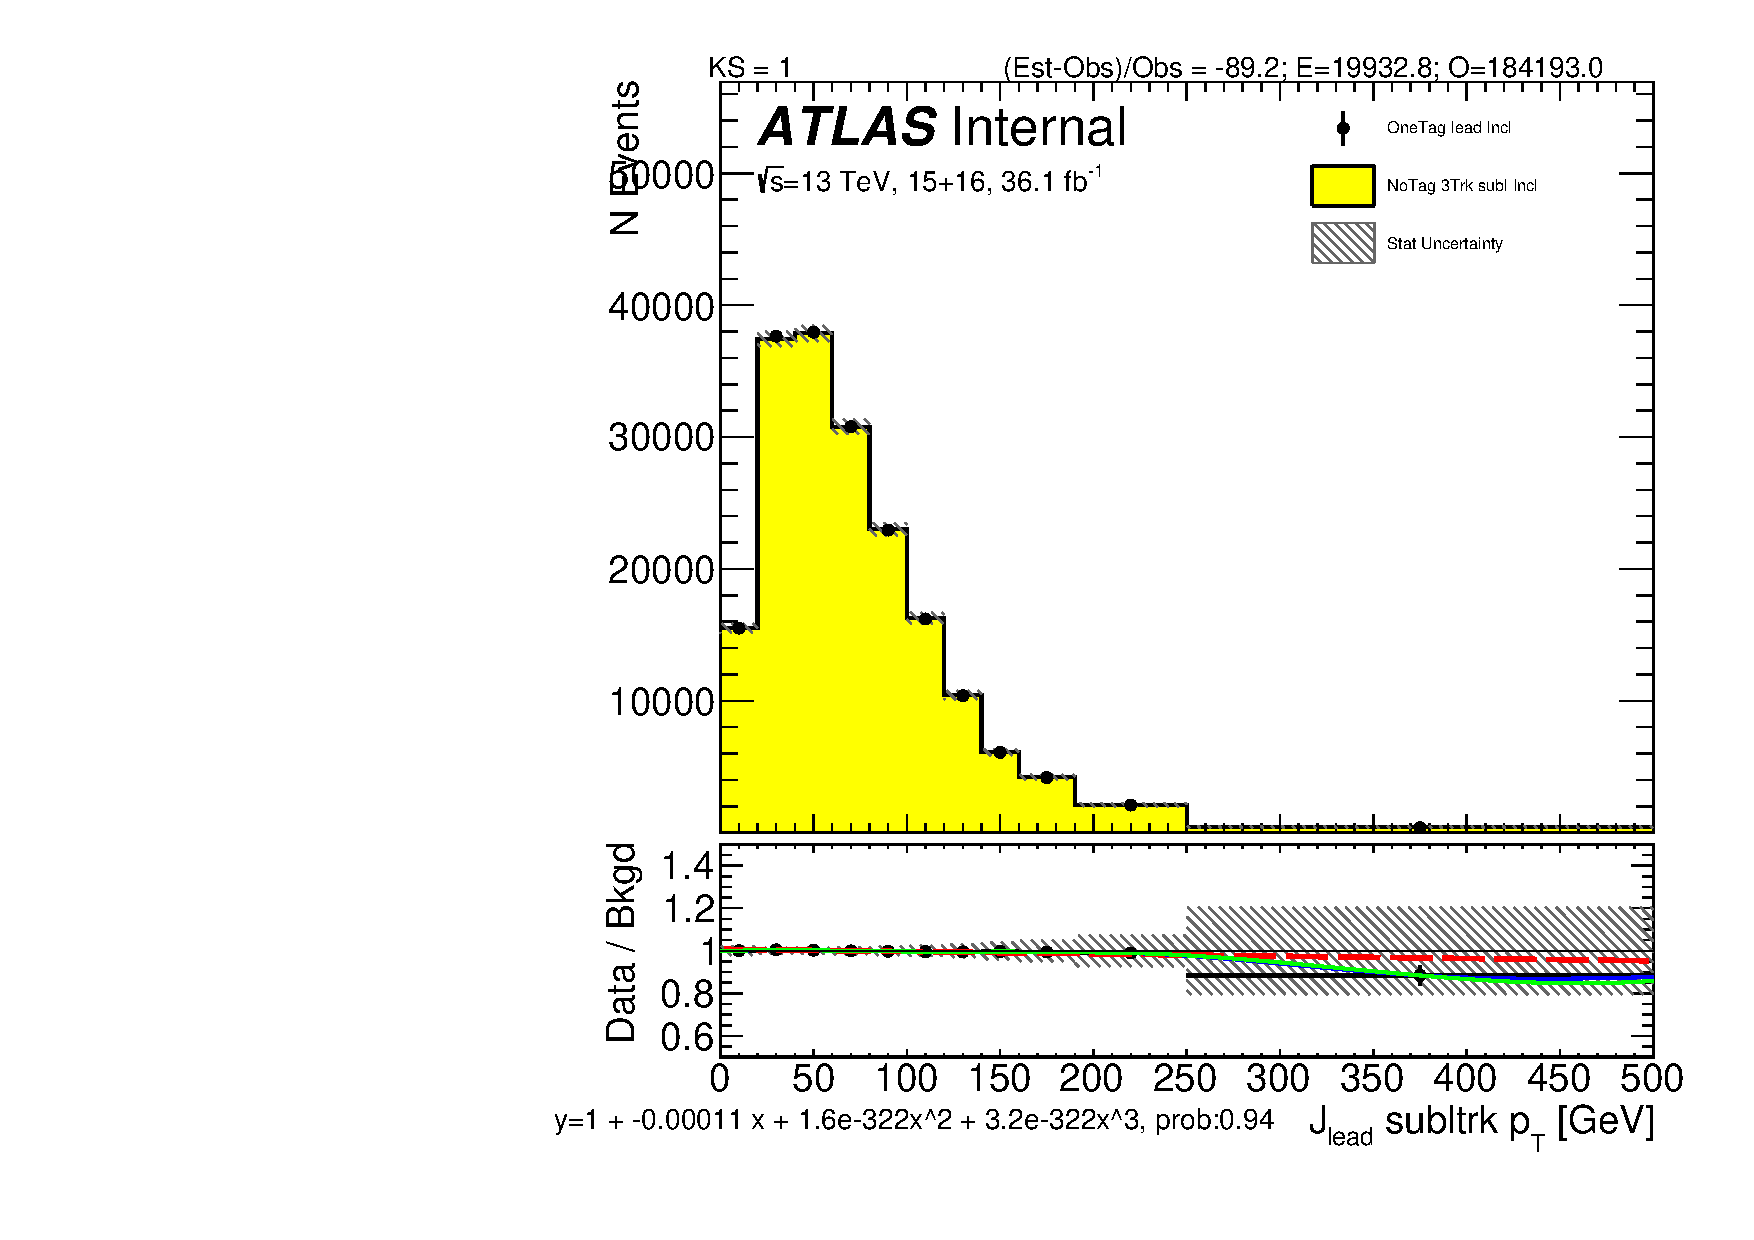
\includegraphics[width=0.32\textwidth,angle=-90]{figures/boosted/Reweight/Fits/Moriond_bkg_3_NoTag_3Trk_subl_Incl_leadHCand_trk1_Pt.pdf} \\
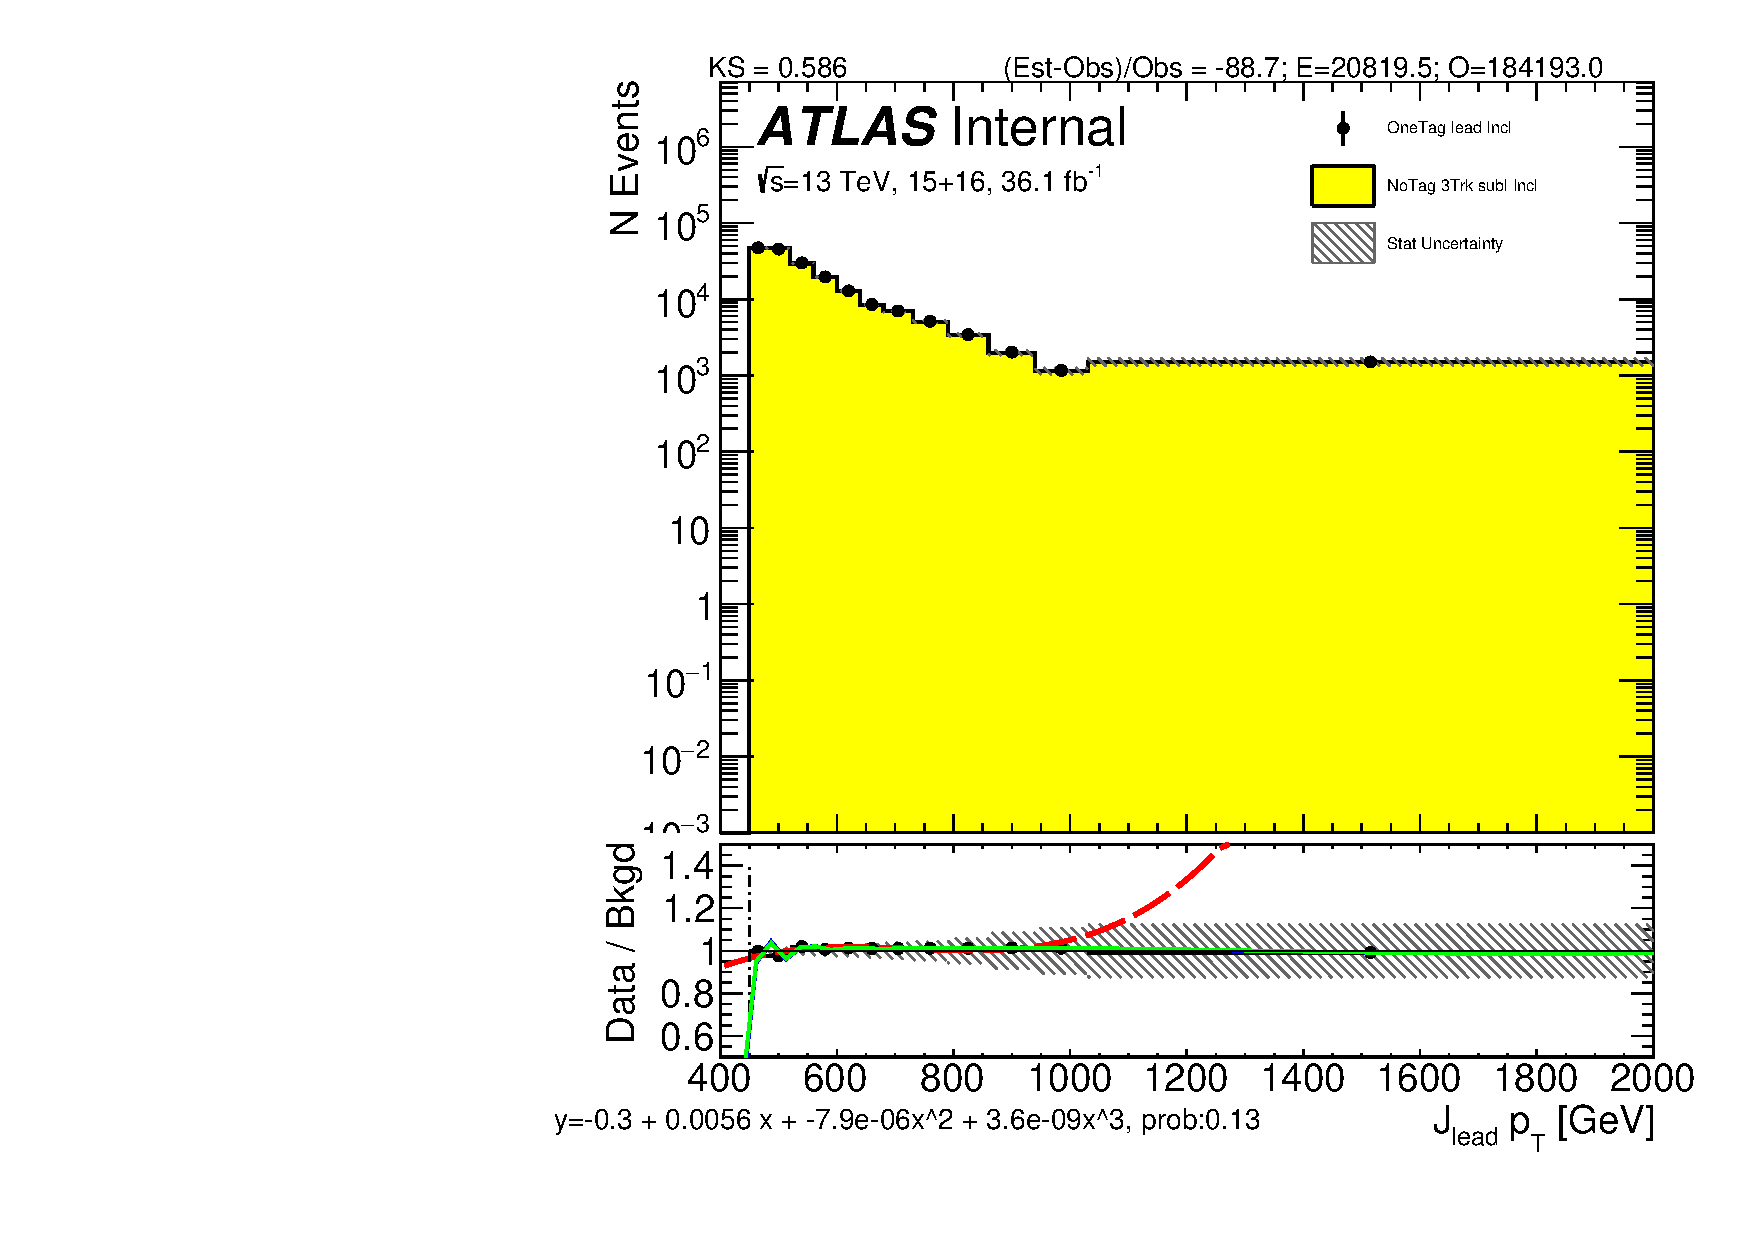
\includegraphics[width=0.32\textwidth,angle=-90]{figures/boosted/Reweight/Fits/Moriond_bkg_9_NoTag_3Trk_subl_Incl_leadHCand_Pt_m_1.pdf}
\includegraphics[width=0.32\textwidth,angle=-90]{figures/boosted/Reweight/Fits/Moriond_bkg_9_NoTag_3Trk_subl_Incl_leadHCand_trk0_Pt.pdf}
\includegraphics[width=0.32\textwidth,angle=-90]{figures/boosted/Reweight/Fits/Moriond_bkg_9_NoTag_3Trk_subl_Incl_leadHCand_trk1_Pt.pdf} \\
\caption{For $3b$ background estimate: the fits to the ratio of the data in the $2b$ category, of the leading Higgs candidate $2b$-tagged events's leading Higgs candidate distributions(black point), over the sublleading Higgs candidate $1b$-tagged events's leading Higgs candidate distributions(yellow). Distributions and fits to the estimated QCD background for large-$R$ jet $p_{T}$ (left),  the large-$R$ jet's leading trackjet $p_T$ (middle), and large-$R$ jet's subleading trackjet $p_T$ (right) are shown.  Figure are shown before reweighting (top row), after the first iteration(second row), after the fourth iteration(third row), and after the last iteration (bottow row). The green line is the spline extrapolation; and the red line is a polynomial fit.}
\label{fig:rw-3b-subl}
\end{center}
\end{figure*}

\begin{figure*}[htbp!]
\begin{center}
\includegraphics[width=0.32\textwidth,angle=-90]{figures/boosted/Reweight/Fits/Moriond_NoTag_4Trk_lead_Incl_sublHCand_Pt_m_1.pdf}
\includegraphics[width=0.32\textwidth,angle=-90]{figures/boosted/Reweight/Fits/Moriond_NoTag_4Trk_lead_Incl_sublHCand_trk0_Pt.pdf}
\includegraphics[width=0.32\textwidth,angle=-90]{figures/boosted/Reweight/Fits/Moriond_NoTag_4Trk_lead_Incl_sublHCand_trk1_Pt.pdf} \\
\includegraphics[width=0.32\textwidth,angle=-90]{figures/boosted/Reweight/Fits/Moriond_bkg_0_NoTag_4Trk_lead_Incl_sublHCand_Pt_m_1.pdf}
\includegraphics[width=0.32\textwidth,angle=-90]{figures/boosted/Reweight/Fits/Moriond_bkg_0_NoTag_4Trk_lead_Incl_sublHCand_trk0_Pt.pdf}
\includegraphics[width=0.32\textwidth,angle=-90]{figures/boosted/Reweight/Fits/Moriond_bkg_0_NoTag_4Trk_lead_Incl_sublHCand_trk1_Pt.pdf} \\
\includegraphics[width=0.32\textwidth,angle=-90]{figures/boosted/Reweight/Fits/Moriond_bkg_3_NoTag_4Trk_lead_Incl_sublHCand_Pt_m_1.pdf}
\includegraphics[width=0.32\textwidth,angle=-90]{figures/boosted/Reweight/Fits/Moriond_bkg_3_NoTag_4Trk_lead_Incl_sublHCand_trk0_Pt.pdf}
\includegraphics[width=0.32\textwidth,angle=-90]{figures/boosted/Reweight/Fits/Moriond_bkg_3_NoTag_4Trk_lead_Incl_sublHCand_trk1_Pt.pdf} \\
\includegraphics[width=0.32\textwidth,angle=-90]{figures/boosted/Reweight/Fits/Moriond_bkg_9_NoTag_4Trk_lead_Incl_sublHCand_Pt_m_1.pdf}
\includegraphics[width=0.32\textwidth,angle=-90]{figures/boosted/Reweight/Fits/Moriond_bkg_9_NoTag_4Trk_lead_Incl_sublHCand_trk0_Pt.pdf}
\includegraphics[width=0.32\textwidth,angle=-90]{figures/boosted/Reweight/Fits/Moriond_bkg_9_NoTag_4Trk_lead_Incl_sublHCand_trk1_Pt.pdf} \\
\caption{For $4b$ background estimate: the fits to the ratio of the data in the $2b$ category, of the sublleading Higgs candidate $2b$-tagged events's subleading Higgs candidate distributions(black point), over the leading Higgs candidate $2b$-tagged events's subleading Higgs candidate distributions(yellow). Distributions and fits to the estimated QCD background for large-$R$ jet $p_{T}$ (left),  the large-$R$ jet's leading trackjet $p_T$ (middle), and large-$R$ jet's subleading trackjet $p_T$ (right) are shown.  Figure are shown before reweighting (top row), after the first iteration(second row), after the fourth iteration(third row), and after the last iteration (bottow row). The green line is the spline extrapolation; and the red line is a polynomial fit.}
\label{fig:rw-4b-lead}
\end{center}
\end{figure*}

\begin{figure*}[htbp!]
\begin{center}
\includegraphics[width=0.32\textwidth,angle=-90]{figures/boosted/Reweight/Fits/Moriond_NoTag_4Trk_subl_Incl_leadHCand_Pt_m_1.pdf}
\includegraphics[width=0.32\textwidth,angle=-90]{figures/boosted/Reweight/Fits/Moriond_NoTag_4Trk_subl_Incl_leadHCand_trk0_Pt.pdf}
\includegraphics[width=0.32\textwidth,angle=-90]{figures/boosted/Reweight/Fits/Moriond_NoTag_4Trk_subl_Incl_leadHCand_trk1_Pt.pdf} \\
\includegraphics[width=0.32\textwidth,angle=-90]{figures/boosted/Reweight/Fits/Moriond_bkg_0_NoTag_4Trk_subl_Incl_leadHCand_Pt_m_1.pdf}
\includegraphics[width=0.32\textwidth,angle=-90]{figures/boosted/Reweight/Fits/Moriond_bkg_0_NoTag_4Trk_subl_Incl_leadHCand_trk0_Pt.pdf}
\includegraphics[width=0.32\textwidth,angle=-90]{figures/boosted/Reweight/Fits/Moriond_bkg_0_NoTag_4Trk_subl_Incl_leadHCand_trk1_Pt.pdf} \\
\includegraphics[width=0.32\textwidth,angle=-90]{figures/boosted/Reweight/Fits/Moriond_bkg_3_NoTag_4Trk_subl_Incl_leadHCand_Pt_m_1.pdf}
\includegraphics[width=0.32\textwidth,angle=-90]{figures/boosted/Reweight/Fits/Moriond_bkg_3_NoTag_4Trk_subl_Incl_leadHCand_trk0_Pt.pdf}
\includegraphics[width=0.32\textwidth,angle=-90]{figures/boosted/Reweight/Fits/Moriond_bkg_3_NoTag_4Trk_subl_Incl_leadHCand_trk1_Pt.pdf} \\
\includegraphics[width=0.32\textwidth,angle=-90]{figures/boosted/Reweight/Fits/Moriond_bkg_9_NoTag_4Trk_subl_Incl_leadHCand_Pt_m_1.pdf}
\includegraphics[width=0.32\textwidth,angle=-90]{figures/boosted/Reweight/Fits/Moriond_bkg_9_NoTag_4Trk_subl_Incl_leadHCand_trk0_Pt.pdf}
\includegraphics[width=0.32\textwidth,angle=-90]{figures/boosted/Reweight/Fits/Moriond_bkg_9_NoTag_4Trk_subl_Incl_leadHCand_trk1_Pt.pdf} \\
\caption{For $4b$ background estimate: the fits to the ratio of the data in the $2b$ category, of the leading Higgs candidate $2b$-tagged events's leading Higgs candidate distributions(black point), over the sublleading Higgs candidate $2b$-tagged events's leading Higgs candidate distributions(yellow). Distributions and fits to the estimated QCD background for large-$R$ jet $p_{T}$ (left),  the large-$R$ jet's leading trackjet $p_T$ (middle), and large-$R$ jet's subleading trackjet $p_T$ (right) are shown.  Figure are shown before reweighting (top row), after the first iteration(second row), after the fourth iteration(third row), and after the last iteration (bottow row). The green line is the spline extrapolation; and the red line is a polynomial fit.}
\label{fig:rw-4b-subl}
\end{center}
\end{figure*}


\pagebreak{}
%%%%%%%%%%%%%%%%%%%%%%%%%%%
\subsubsection{Reweighting Results Comparison in Sideband and Control Region}
\label{sec:boosted-Reweight-compare}

%%\paragraph{}
A comparison of the Sideband shapes before and after reweighting for $2bs$, $3b$ and $4b$ can be seen in Figures~\ref{fig:rw-2bs-comp-sb},~\ref{fig:rw-3b-comp-sb}, and ~\ref{fig:rw-4b-comp-sb}. Also, a comparison of the Control Region shapes before and after reweighting for $2bs$, $3b$ and $4b$ can be seen in Figures~\ref{fig:rw-2bs-comp-cr},~\ref{fig:rw-3b-comp-cr}, and ~\ref{fig:rw-4b-comp-cr}. In almost all cases, both the reweighted/non-reweighted prediction agrees fairly well with the data, and the reweighted plots' KS score improved from non-reweighted distributions. 

%%%%%%%%%%%%%%%%%%%%%%%%%%%
\begin{figure*}[htbp!]
\begin{center}
\includegraphics[width=0.31\textwidth,angle=-90]{figures/boosted/Prereweight/Moriond_TwoTag_split_Sideband_mHH_l_1.pdf}
\includegraphics[width=0.31\textwidth,angle=-90]{figures/boosted/Sideband/b77_TwoTag_split_Sideband_mHH_l_1.pdf}\\
\includegraphics[width=0.31\textwidth,angle=-90]{figures/boosted/Prereweight/Moriond_TwoTag_split_Sideband_leadHCand_Pt_m.pdf}
\includegraphics[width=0.31\textwidth,angle=-90]{figures/boosted/Sideband/b77_TwoTag_split_Sideband_leadHCand_Pt_m.pdf}\\
\includegraphics[width=0.31\textwidth,angle=-90]{figures/boosted/Prereweight/Moriond_TwoTag_split_Sideband_leadHCand_trk0_Pt.pdf}
\includegraphics[width=0.31\textwidth,angle=-90]{figures/boosted/Sideband/b77_TwoTag_split_Sideband_leadHCand_trk0_Pt.pdf}\\
\includegraphics[width=0.31\textwidth,angle=-90]{figures/boosted/Prereweight/Moriond_TwoTag_split_Sideband_sublHCand_trk0_Pt.pdf}
\includegraphics[width=0.31\textwidth,angle=-90]{figures/boosted/Sideband/b77_TwoTag_split_Sideband_sublHCand_trk0_Pt.pdf}\\
\caption{Reweighted $2bs$ Sideband region predictions comaprison. Top row is the dijet Mass, second row is leading large-$R$ jet $p_{T}$, third row is the leading large-$R$ jet's leading trackjet $p_T$ and the last row subleading large-$R$ jet's leading trackjet $p_T$. On the left are the distributions before reweighting, and on the right are the distributions after reweighting.}
\label{fig:rw-2bs-comp-sb}
\end{center}
\end{figure*}


\begin{figure*}[htbp!]
\begin{center}
\includegraphics[width=0.31\textwidth,angle=-90]{figures/boosted/Prereweight/Moriond_ThreeTag_Sideband_mHH_l_1.pdf}
\includegraphics[width=0.31\textwidth,angle=-90]{figures/boosted/Sideband/b77_ThreeTag_Sideband_mHH_l_1.pdf}\\
\includegraphics[width=0.31\textwidth,angle=-90]{figures/boosted/Prereweight/Moriond_ThreeTag_Sideband_leadHCand_Pt_m.pdf}
\includegraphics[width=0.31\textwidth,angle=-90]{figures/boosted/Sideband/b77_ThreeTag_Sideband_leadHCand_Pt_m.pdf}\\
\includegraphics[width=0.31\textwidth,angle=-90]{figures/boosted/Prereweight/Moriond_ThreeTag_Sideband_leadHCand_trk0_Pt.pdf}
\includegraphics[width=0.31\textwidth,angle=-90]{figures/boosted/Sideband/b77_ThreeTag_Sideband_leadHCand_trk0_Pt.pdf}\\
\includegraphics[width=0.31\textwidth,angle=-90]{figures/boosted/Prereweight/Moriond_ThreeTag_Sideband_sublHCand_trk0_Pt.pdf}
\includegraphics[width=0.31\textwidth,angle=-90]{figures/boosted/Sideband/b77_ThreeTag_Sideband_sublHCand_trk0_Pt.pdf}\\
\caption{Reweighted $3b$ Sideband region predictions comaprison. Top row is the dijet Mass, second row is leading large-$R$ jet $p_{T}$, third row is the leading large-$R$ jet's leading trackjet $p_T$ and the last row subleading large-$R$ jet's leading trackjet $p_T$. On the left are the distributions before reweighting, and on the right are the distributions after reweighting.}
\label{fig:rw-3b-comp-sb}
\end{center}
\end{figure*}


\begin{figure*}[htbp!]
\begin{center}
\includegraphics[width=0.31\textwidth,angle=-90]{figures/boosted/Prereweight/Moriond_FourTag_Sideband_mHH_l_1.pdf}
\includegraphics[width=0.31\textwidth,angle=-90]{figures/boosted/Sideband/b77_FourTag_Sideband_mHH_l_1.pdf}\\
\includegraphics[width=0.31\textwidth,angle=-90]{figures/boosted/Prereweight/Moriond_FourTag_Sideband_leadHCand_Pt_m.pdf}
\includegraphics[width=0.31\textwidth,angle=-90]{figures/boosted/Sideband/b77_FourTag_Sideband_leadHCand_Pt_m.pdf}\\
\includegraphics[width=0.31\textwidth,angle=-90]{figures/boosted/Prereweight/Moriond_FourTag_Sideband_leadHCand_trk0_Pt.pdf}
\includegraphics[width=0.31\textwidth,angle=-90]{figures/boosted/Sideband/b77_FourTag_Sideband_leadHCand_trk0_Pt.pdf}\\
\includegraphics[width=0.31\textwidth,angle=-90]{figures/boosted/Prereweight/Moriond_FourTag_Sideband_sublHCand_trk0_Pt.pdf}
\includegraphics[width=0.31\textwidth,angle=-90]{figures/boosted/Sideband/b77_FourTag_Sideband_sublHCand_trk0_Pt.pdf}\\
\caption{Reweighted $4b$ Sideband region predictions comaprison. Top row is the dijet Mass, second row is leading large-$R$ jet $p_{T}$, third row is the leading large-$R$ jet's leading trackjet $p_T$ and the last row subleading large-$R$ jet's leading trackjet $p_T$. On the left are the distributions before reweighting, and on the right are the distributions after reweighting.}
\label{fig:rw-4b-comp-sb}
\end{center}
\end{figure*}



%%%%%%%%%%%%%%%%%%%%%%%%%%%
\begin{figure*}[htbp!]
\begin{center}
\includegraphics[width=0.31\textwidth,angle=-90]{figures/boosted/Prereweight/Moriond_TwoTag_split_Control_mHH_l_1.pdf}
\includegraphics[width=0.31\textwidth,angle=-90]{figures/boosted/Control/b77_TwoTag_split_Control_mHH_l_1.pdf}\\
\includegraphics[width=0.31\textwidth,angle=-90]{figures/boosted/Prereweight/Moriond_TwoTag_split_Control_leadHCand_Pt_m.pdf}
\includegraphics[width=0.31\textwidth,angle=-90]{figures/boosted/Control/b77_TwoTag_split_Control_leadHCand_Pt_m.pdf}\\
\includegraphics[width=0.31\textwidth,angle=-90]{figures/boosted/Prereweight/Moriond_TwoTag_split_Control_leadHCand_trk0_Pt.pdf}
\includegraphics[width=0.31\textwidth,angle=-90]{figures/boosted/Control/b77_TwoTag_split_Control_leadHCand_trk0_Pt.pdf}\\
\includegraphics[width=0.31\textwidth,angle=-90]{figures/boosted/Prereweight/Moriond_TwoTag_split_Control_sublHCand_trk0_Pt.pdf}
\includegraphics[width=0.31\textwidth,angle=-90]{figures/boosted/Control/b77_TwoTag_split_Control_sublHCand_trk0_Pt.pdf}\\
\caption{Reweighted $2bs$ Control region predictions comaprison. Top row is the dijet Mass, second row is leading large-$R$ jet $p_{T}$, third row is the leading large-$R$ jet's leading trackjet $p_T$ and the last row subleading large-$R$ jet's leading trackjet $p_T$. On the left are the distributions before reweighting, and on the right are the distributions after reweighting.}
\label{fig:rw-2bs-comp-cr}
\end{center}
\end{figure*}


\begin{figure*}[htbp!]
\begin{center}
\includegraphics[width=0.31\textwidth,angle=-90]{figures/boosted/Prereweight/Moriond_ThreeTag_Control_mHH_l_1.pdf}
\includegraphics[width=0.31\textwidth,angle=-90]{figures/boosted/Control/b77_ThreeTag_Control_mHH_l_1.pdf}\\
\includegraphics[width=0.31\textwidth,angle=-90]{figures/boosted/Prereweight/Moriond_ThreeTag_Control_leadHCand_Pt_m.pdf}
\includegraphics[width=0.31\textwidth,angle=-90]{figures/boosted/Control/b77_ThreeTag_Control_leadHCand_Pt_m.pdf}\\
\includegraphics[width=0.31\textwidth,angle=-90]{figures/boosted/Prereweight/Moriond_ThreeTag_Control_leadHCand_trk0_Pt.pdf}
\includegraphics[width=0.31\textwidth,angle=-90]{figures/boosted/Control/b77_ThreeTag_Control_leadHCand_trk0_Pt.pdf}\\
\includegraphics[width=0.31\textwidth,angle=-90]{figures/boosted/Prereweight/Moriond_ThreeTag_Control_sublHCand_trk0_Pt.pdf}
\includegraphics[width=0.31\textwidth,angle=-90]{figures/boosted/Control/b77_ThreeTag_Control_sublHCand_trk0_Pt.pdf}\\
\caption{Reweighted $3b$ Control region predictions comaprison. Top row is the dijet Mass, second row is leading large-$R$ jet $p_{T}$, third row is the leading large-$R$ jet's leading trackjet $p_T$ and the last row subleading large-$R$ jet's leading trackjet $p_T$. On the left are the distributions before reweighting, and on the right are the distributions after reweighting.}
\label{fig:rw-3b-comp-cr}
\end{center}
\end{figure*}


\begin{figure*}[htbp!]
\begin{center}
\includegraphics[width=0.31\textwidth,angle=-90]{figures/boosted/Prereweight/Moriond_FourTag_Control_mHH_l_1.pdf}
\includegraphics[width=0.31\textwidth,angle=-90]{figures/boosted/Control/b77_FourTag_Control_mHH_l_1.pdf}\\
\includegraphics[width=0.31\textwidth,angle=-90]{figures/boosted/Prereweight/Moriond_FourTag_Control_leadHCand_Pt_m.pdf}
\includegraphics[width=0.31\textwidth,angle=-90]{figures/boosted/Control/b77_FourTag_Control_leadHCand_Pt_m.pdf}\\
\includegraphics[width=0.31\textwidth,angle=-90]{figures/boosted/Prereweight/Moriond_FourTag_Control_leadHCand_trk0_Pt.pdf}
\includegraphics[width=0.31\textwidth,angle=-90]{figures/boosted/Control/b77_FourTag_Control_leadHCand_trk0_Pt.pdf}\\
\includegraphics[width=0.31\textwidth,angle=-90]{figures/boosted/Prereweight/Moriond_FourTag_Control_sublHCand_trk0_Pt.pdf}
\includegraphics[width=0.31\textwidth,angle=-90]{figures/boosted/Control/b77_FourTag_Control_sublHCand_trk0_Pt.pdf}\\
\caption{Reweighted $4b$ Control region predictions comaprison. Top row is the dijet Mass, second row is leading large-$R$ jet $p_{T}$, third row is the leading large-$R$ jet's leading trackjet $p_T$ and the last row subleading large-$R$ jet's leading trackjet $p_T$. On the left are the distributions before reweighting, and on the right are the distributions after reweighting.}
\label{fig:rw-4b-comp-cr}
\end{center}
\end{figure*}

\clearpage
